\documentclass[twoside]{book}

% Packages required by doxygen
\usepackage{calc}
\usepackage{doxygen}
\usepackage{graphicx}
\usepackage[utf8]{inputenc}
\usepackage{makeidx}
\usepackage{multicol}
\usepackage{multirow}
\usepackage{textcomp}
\usepackage[table]{xcolor}

% Font selection
\usepackage[T1]{fontenc}
\usepackage{mathptmx}
\usepackage[scaled=.90]{helvet}
\usepackage{courier}
\usepackage{amssymb}
\usepackage{sectsty}
\renewcommand{\familydefault}{\sfdefault}
\allsectionsfont{%
  \fontseries{bc}\selectfont%
  \color{darkgray}%
}
\renewcommand{\DoxyLabelFont}{%
  \fontseries{bc}\selectfont%
  \color{darkgray}%
}

% Page & text layout
\usepackage{geometry}
\geometry{%
  a4paper,%
  top=2.5cm,%
  bottom=2.5cm,%
  left=2.5cm,%
  right=2.5cm%
}
\tolerance=750
\hfuzz=15pt
\hbadness=750
\setlength{\emergencystretch}{15pt}
\setlength{\parindent}{0cm}
\setlength{\parskip}{0.2cm}
\makeatletter
\renewcommand{\paragraph}{%
  \@startsection{paragraph}{4}{0ex}{-1.0ex}{1.0ex}{%
    \normalfont\normalsize\bfseries\SS@parafont%
  }%
}
\renewcommand{\subparagraph}{%
  \@startsection{subparagraph}{5}{0ex}{-1.0ex}{1.0ex}{%
    \normalfont\normalsize\bfseries\SS@subparafont%
  }%
}
\makeatother

% Headers & footers
\usepackage{fancyhdr}
\pagestyle{fancyplain}
\fancyhead[LE]{\fancyplain{}{\bfseries\thepage}}
\fancyhead[CE]{\fancyplain{}{}}
\fancyhead[RE]{\fancyplain{}{\bfseries\leftmark}}
\fancyhead[LO]{\fancyplain{}{\bfseries\rightmark}}
\fancyhead[CO]{\fancyplain{}{}}
\fancyhead[RO]{\fancyplain{}{\bfseries\thepage}}
\fancyfoot[LE]{\fancyplain{}{}}
\fancyfoot[CE]{\fancyplain{}{}}
\fancyfoot[RE]{\fancyplain{}{\bfseries\scriptsize Generated on Sun Nov 12 2017 16\-:14\-:53 for S\-Q\-Lite\-X\-X by Doxygen }}
\fancyfoot[LO]{\fancyplain{}{\bfseries\scriptsize Generated on Sun Nov 12 2017 16\-:14\-:53 for S\-Q\-Lite\-X\-X by Doxygen }}
\fancyfoot[CO]{\fancyplain{}{}}
\fancyfoot[RO]{\fancyplain{}{}}
\renewcommand{\footrulewidth}{0.4pt}
\renewcommand{\chaptermark}[1]{%
  \markboth{#1}{}%
}
\renewcommand{\sectionmark}[1]{%
  \markright{\thesection\ #1}%
}

% Indices & bibliography
\usepackage{natbib}
\usepackage[titles]{tocloft}
\setcounter{tocdepth}{3}
\setcounter{secnumdepth}{5}
\makeindex

% Hyperlinks (required, but should be loaded last)
\usepackage{ifpdf}
\ifpdf
  \usepackage[pdftex,pagebackref=true]{hyperref}
\else
  \usepackage[ps2pdf,pagebackref=true]{hyperref}
\fi
\hypersetup{%
  colorlinks=true,%
  linkcolor=blue,%
  citecolor=blue,%
  unicode%
}

% Custom commands
\newcommand{\clearemptydoublepage}{%
  \newpage{\pagestyle{empty}\cleardoublepage}%
}


%===== C O N T E N T S =====

\begin{document}

% Titlepage & ToC
\hypersetup{pageanchor=false}
\pagenumbering{roman}
\begin{titlepage}
\vspace*{7cm}
\begin{center}%
{\Large S\-Q\-Lite\-X\-X \\[1ex]\large 0.\-1.\-0 }\\
\vspace*{1cm}
{\large Generated by Doxygen 1.8.6}\\
\vspace*{0.5cm}
{\small Sun Nov 12 2017 16:14:53}\\
\end{center}
\end{titlepage}
\clearemptydoublepage
\tableofcontents
\clearemptydoublepage
\pagenumbering{arabic}
\hypersetup{pageanchor=true}

%--- Begin generated contents ---
\chapter{Main Page}
\label{index}\hypertarget{index}{}\href{https://github.com/maxxboehme/SQLiteXX/blob/master/LICENSE.txt}{\tt !\mbox{[}License\mbox{]}(https\-://img.\-shields.\-io/badge/license-\/\-M\-I\-T-\/blue.\-svg)} \href{https://travis-ci.org/maxxboehme/SQLiteXX}{\tt !\mbox{[}Travis C\-I Linux/\-Mac Build Status\mbox{]}(https\-://travis-\/ci.\-org/maxxboehme/\-S\-Q\-Lite\-X\-X.\-svg?branch=master)} \href{https://ci.appveyor.com/project/maxxboehme/sqlitexx/branch/master}{\tt !\mbox{[}App\-Veyor Windows Build status\mbox{]}(https\-://ci.\-appveyor.\-com/api/projects/status/wkrlgfv2p5mm5cgg/branch/master?svg=true)} \href{https://coveralls.io/github/maxxboehme/SQLiteXX}{\tt !\mbox{[}Coverage Status\mbox{]}(https\-://coveralls.\-io/repos/github/maxxboehme/\-S\-Q\-Lite\-X\-X/badge.\-svg)}

\subsection*{What is S\-Q\-Lite\-X\-X}

A C++ wrapper for sqlite3 that uses features in C++14.

\subsection*{How to use it}

The following links will direct you to helpful documents on how to use S\-Q\-Lite\-X\-X.


\begin{DoxyItemize}
\item https\-://github.com/maxxboehme/\-S\-Q\-Lite\-X\-X/blob/master/docs/tutorial.\-md \char`\"{}\-Tutorial\char`\"{} -\/ Getting Started
\item \href{https://maxxboehme.github.io/SQLiteXX/doxygen/html}{\tt Doxygen} -\/ Documentation for the A\-P\-I
\item https\-://github.com/maxxboehme/\-S\-Q\-Lite\-X\-X/blob/master/docs/\-Read\-Me.\-md \char`\"{}\-Reference\char`\"{} -\/ all the details
\end{DoxyItemize}

\subsection*{How to build it}

You will need a compiler that supports C++14. The Travis-\/\-C\-I Y\-A\-M\-L file shows some of the supported compilers.

\subsection*{More}


\begin{DoxyItemize}
\item Issues and bugs can be raised on the \href{https://github.com/maxxboehme/SQLiteXX/issues}{\tt Issue tracker on Github} 
\end{DoxyItemize}
\chapter{Namespace Index}
\section{Namespace List}
Here is a list of all documented namespaces with brief descriptions\-:\begin{DoxyCompactList}
\item\contentsline{section}{\hyperlink{a00038}{S\-Q\-Lite} \\*S\-Q\-Lite\-X\-X classes and functions are defined in this namespace }{\pageref{a00038}}{}
\end{DoxyCompactList}

\chapter{Hierarchical Index}
\section{Class Hierarchy}
This inheritance list is sorted roughly, but not completely, alphabetically\-:\begin{DoxyCompactList}
\item \contentsline{section}{sqlite\-:\-:backup}{\pageref{a00001}}{}
\item \contentsline{section}{sqlite\-:\-:blob}{\pageref{a00002}}{}
\item \contentsline{section}{sqlite\-:\-:dbconnection}{\pageref{a00004}}{}
\item \contentsline{section}{sqlite\-:\-:exception}{\pageref{a00006}}{}
\begin{DoxyCompactList}
\item \contentsline{section}{sqlite\-:\-:busy\-\_\-exception}{\pageref{a00003}}{}
\end{DoxyCompactList}
\item \contentsline{section}{sqlite\-:\-:mutex}{\pageref{a00009}}{}
\item \contentsline{section}{sqlite\-:\-:reader$<$ T $>$}{\pageref{a00010}}{}
\item \contentsline{section}{sqlite\-:\-:reader$<$ row $>$}{\pageref{a00010}}{}
\begin{DoxyCompactList}
\item \contentsline{section}{sqlite\-:\-:row}{\pageref{a00011}}{}
\end{DoxyCompactList}
\item \contentsline{section}{sqlite\-:\-:reader$<$ statement $>$}{\pageref{a00010}}{}
\begin{DoxyCompactList}
\item \contentsline{section}{sqlite\-:\-:statement}{\pageref{a00013}}{}
\end{DoxyCompactList}
\item \contentsline{section}{sqlite\-:\-:row\-\_\-iterator}{\pageref{a00012}}{}
\item \contentsline{section}{sqlite\-:\-:transaction}{\pageref{a00014}}{}
\begin{DoxyCompactList}
\item \contentsline{section}{sqlite\-:\-:deferred\-\_\-transaction}{\pageref{a00005}}{}
\item \contentsline{section}{sqlite\-:\-:exclusive\-\_\-transaction}{\pageref{a00007}}{}
\item \contentsline{section}{sqlite\-:\-:immediate\-\_\-transaction}{\pageref{a00008}}{}
\end{DoxyCompactList}
\item \contentsline{section}{sqlite\-:\-:value}{\pageref{a00015}}{}
\end{DoxyCompactList}

\chapter{Class Index}
\section{Class List}
Here are the classes, structs, unions and interfaces with brief descriptions\-:\begin{DoxyCompactList}
\item\contentsline{section}{\hyperlink{a00001}{sqlite\-::backup} \\*Used to aid in the process of backing up a database }{\pageref{a00001}}{}
\item\contentsline{section}{\hyperlink{a00002}{sqlite\-::blob} \\*A \char`\"{}\-Binary Large O\-Bject\char`\"{} }{\pageref{a00002}}{}
\item\contentsline{section}{\hyperlink{a00003}{sqlite\-::busy\-\_\-exception} \\*Encapsulation of the S\-Q\-L\-I\-T\-E\-\_\-\-B\-U\-S\-Y error code derived from S\-Q\-Lite\-::\-Exception }{\pageref{a00003}}{}
\item\contentsline{section}{\hyperlink{a00004}{sqlite\-::dbconnection} \\*Class that represents a connection to a database }{\pageref{a00004}}{}
\item\contentsline{section}{\hyperlink{a00005}{sqlite\-::deferred\-\_\-transaction} \\*R\-A\-I\-I encapsulation of the \hyperlink{a00038}{S\-Q\-Lite} deferred transaction }{\pageref{a00005}}{}
\item\contentsline{section}{\hyperlink{a00006}{sqlite\-::exception} \\*Encapsulation of the error code and message from S\-Q\-Lite3, based on std\-::runtime\-\_\-error }{\pageref{a00006}}{}
\item\contentsline{section}{\hyperlink{a00007}{sqlite\-::exclusive\-\_\-transaction} \\*R\-A\-I\-I encapsulation of the \hyperlink{a00038}{S\-Q\-Lite} exclusive transaction }{\pageref{a00007}}{}
\item\contentsline{section}{\hyperlink{a00008}{sqlite\-::immediate\-\_\-transaction} \\*R\-A\-I\-I encapsulation of the \hyperlink{a00038}{S\-Q\-Lite} immediate transaction }{\pageref{a00008}}{}
\item\contentsline{section}{\hyperlink{a00009}{sqlite\-::mutex} \\*Helps with serializing access to a database connection }{\pageref{a00009}}{}
\item\contentsline{section}{\hyperlink{a00010}{sqlite\-::reader$<$ T $>$} \\*Base class used to help with reading \char`\"{}sqlite3\-\_\-stmt\char`\"{} information }{\pageref{a00010}}{}
\item\contentsline{section}{\hyperlink{a00011}{sqlite\-::row} \\*Represents a returned row when stepping through a \char`\"{}\-S\-E\-L\-E\-C\-T\char`\"{} statement }{\pageref{a00011}}{}
\item\contentsline{section}{\hyperlink{a00012}{sqlite\-::row\-\_\-iterator} \\*Helps when iterating over rows in a \char`\"{}\-S\-E\-L\-E\-C\-T\char`\"{} statement }{\pageref{a00012}}{}
\item\contentsline{section}{\hyperlink{a00013}{sqlite\-::statement} \\*Represents a single S\-Q\-L statement that has been compiled into binary form and is ready to be evaluated, aka \char`\"{}sqlite3\-\_\-stmt\char`\"{} }{\pageref{a00013}}{}
\item\contentsline{section}{\hyperlink{a00014}{sqlite\-::transaction} \\*R\-A\-I\-I encapsulation of the \hyperlink{a00038}{S\-Q\-Lite} Transactions }{\pageref{a00014}}{}
\item\contentsline{section}{\hyperlink{a00015}{sqlite\-::value} \\*A \hyperlink{a00038}{S\-Q\-Lite} dynamically typed value object, aka \char`\"{}sqlite3\-\_\-value\char`\"{} }{\pageref{a00015}}{}
\end{DoxyCompactList}

\chapter{File Index}
\section{File List}
Here is a list of all documented files with brief descriptions\-:\begin{DoxyCompactList}
\item\contentsline{section}{src/{\bfseries Backup.\-cpp} }{\pageref{a00017}}{}
\item\contentsline{section}{src/\hyperlink{a00018}{Backup.\-h} }{\pageref{a00018}}{}
\item\contentsline{section}{src/{\bfseries Blob.\-cpp} }{\pageref{a00019}}{}
\item\contentsline{section}{src/\hyperlink{a00020}{Blob.\-h} }{\pageref{a00020}}{}
\item\contentsline{section}{src/{\bfseries D\-B\-Connection.\-cpp} }{\pageref{a00021}}{}
\item\contentsline{section}{src/\hyperlink{a00022}{D\-B\-Connection.\-h} }{\pageref{a00022}}{}
\item\contentsline{section}{src/{\bfseries Exception.\-cpp} }{\pageref{a00023}}{}
\item\contentsline{section}{src/\hyperlink{a00024}{Exception.\-h} }{\pageref{a00024}}{}
\item\contentsline{section}{src/{\bfseries Functions.\-h} }{\pageref{a00025}}{}
\item\contentsline{section}{src/{\bfseries Mutex.\-cpp} }{\pageref{a00026}}{}
\item\contentsline{section}{src/\hyperlink{a00027}{Mutex.\-h} }{\pageref{a00027}}{}
\item\contentsline{section}{src/\hyperlink{a00028}{Open.\-h} }{\pageref{a00028}}{}
\item\contentsline{section}{src/\hyperlink{a00029}{S\-Q\-Lite\-Enums.\-h} }{\pageref{a00029}}{}
\item\contentsline{section}{src/\hyperlink{a00030}{S\-Q\-Lite\-X\-X.\-h} }{\pageref{a00030}}{}
\item\contentsline{section}{src/{\bfseries Statement.\-cpp} }{\pageref{a00031}}{}
\item\contentsline{section}{src/\hyperlink{a00032}{Statement.\-h} }{\pageref{a00032}}{}
\item\contentsline{section}{src/{\bfseries Transaction.\-cpp} }{\pageref{a00033}}{}
\item\contentsline{section}{src/\hyperlink{a00034}{Transaction.\-h} }{\pageref{a00034}}{}
\item\contentsline{section}{src/{\bfseries Utilities.\-h} }{\pageref{a00035}}{}
\item\contentsline{section}{src/{\bfseries Value.\-cpp} }{\pageref{a00036}}{}
\item\contentsline{section}{src/\hyperlink{a00037}{Value.\-h} }{\pageref{a00037}}{}
\end{DoxyCompactList}

\chapter{Namespace Documentation}
\hypertarget{a00038}{\section{S\-Q\-Lite Namespace Reference}
\label{a00038}\index{S\-Q\-Lite@{S\-Q\-Lite}}
}


S\-Q\-Lite\-X\-X classes and functions are defined in this namespace.  




\subsection{Detailed Description}
S\-Q\-Lite\-X\-X classes and functions are defined in this namespace. 
\chapter{Class Documentation}
\hypertarget{a00001}{\section{S\-Q\-Lite\-:\-:Busy\-Exception Class Reference}
\label{a00001}\index{S\-Q\-Lite\-::\-Busy\-Exception@{S\-Q\-Lite\-::\-Busy\-Exception}}
}


Encapsulation of the S\-Q\-L\-I\-T\-E\-\_\-\-B\-U\-S\-Y error code derived from \hyperlink{a00003}{S\-Q\-Lite\-::\-Exception}.  




{\ttfamily \#include $<$Exception.\-h$>$}

Inheritance diagram for S\-Q\-Lite\-:\-:Busy\-Exception\-:\begin{figure}[H]
\begin{center}
\leavevmode
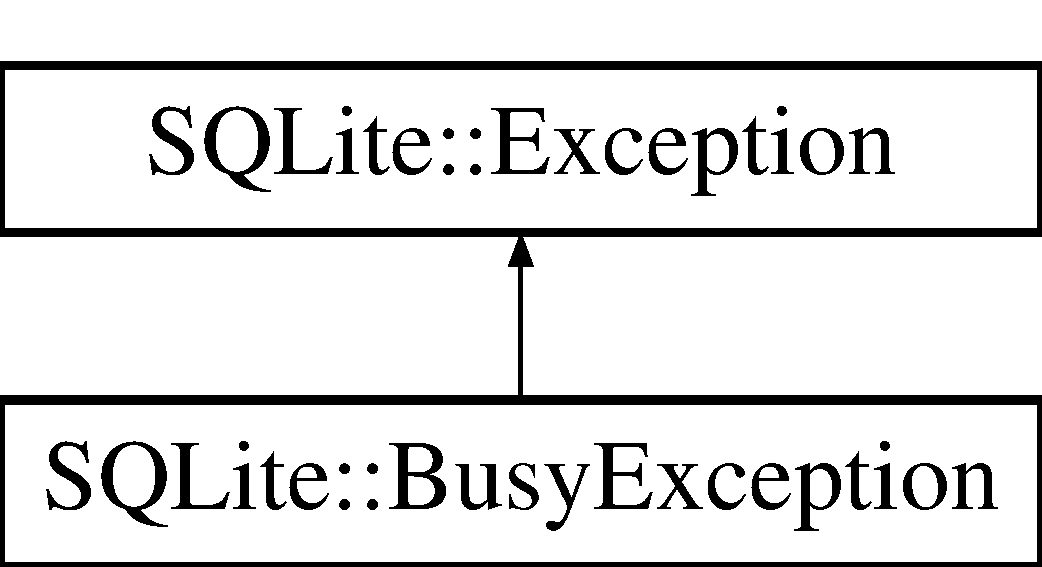
\includegraphics[height=2.000000cm]{a00001}
\end{center}
\end{figure}


\subsection{Detailed Description}
Encapsulation of the S\-Q\-L\-I\-T\-E\-\_\-\-B\-U\-S\-Y error code derived from \hyperlink{a00003}{S\-Q\-Lite\-::\-Exception}. 



Definition at line 33 of file Exception.\-h.



The documentation for this class was generated from the following file\-:\begin{DoxyCompactItemize}
\item 
src/Exception.\-h\end{DoxyCompactItemize}

\hypertarget{a00002}{\section{sqlite\-:\-:blob Class Reference}
\label{a00002}\index{sqlite\-::blob@{sqlite\-::blob}}
}


A \char`\"{}\-Binary Large O\-Bject\char`\"{}.  




{\ttfamily \#include $<$Blob.\-h$>$}

\subsection*{Public Member Functions}
\begin{DoxyCompactItemize}
\item 
\hyperlink{a00002_ad3d7146a3081de7c96a37b9641f83dd6}{blob} (const void $\ast$\hyperlink{a00002_ad9fc3eb820ef6fa64a4a03224b9dc3de}{data}, const size\-\_\-t \hyperlink{a00002_a28b69b40596ded278607604396b86c97}{size})
\begin{DoxyCompactList}\small\item\em Constructs a blob object with contents of data. \end{DoxyCompactList}\item 
\hyperlink{a00002_a1f1bca1ecf4615c4948f3af74814abde}{blob} (const \hyperlink{a00002}{blob} \&other)
\begin{DoxyCompactList}\small\item\em Copy constructor. \end{DoxyCompactList}\item 
\hyperlink{a00002_a78501ec4704d95d590457eacc63f39b6}{blob} (\hyperlink{a00002}{blob} \&\&other)
\begin{DoxyCompactList}\small\item\em Move constructor. \end{DoxyCompactList}\item 
\hyperlink{a00002}{blob} \& \hyperlink{a00002_a1962255cded865181174a67351d58fb8}{operator=} (const \hyperlink{a00002}{blob} \&other)
\begin{DoxyCompactList}\small\item\em Copy assignment operator. \end{DoxyCompactList}\item 
\hyperlink{a00002}{blob} \& \hyperlink{a00002_a93a890b30c970d76fc51ad7ed4bb36c1}{operator=} (\hyperlink{a00002}{blob} \&\&other)
\begin{DoxyCompactList}\small\item\em Move assignment operator. \end{DoxyCompactList}\item 
const void $\ast$ \hyperlink{a00002_ad9fc3eb820ef6fa64a4a03224b9dc3de}{data} () const 
\begin{DoxyCompactList}\small\item\em The raw data of the blob's contents. \end{DoxyCompactList}\item 
size\-\_\-t \hyperlink{a00002_a28b69b40596ded278607604396b86c97}{size} () const 
\begin{DoxyCompactList}\small\item\em Used to get the size of the contained 'blob'. \end{DoxyCompactList}\end{DoxyCompactItemize}


\subsection{Detailed Description}
A \char`\"{}\-Binary Large O\-Bject\char`\"{}. 

A collection of binary data stored as a single entity in a database management system. blobs are typically images, audo or other multimedia object though they can be any form of data. 

Definition at line 20 of file Blob.\-h.



\subsection{Constructor \& Destructor Documentation}
\hypertarget{a00002_ad3d7146a3081de7c96a37b9641f83dd6}{\index{sqlite\-::blob@{sqlite\-::blob}!blob@{blob}}
\index{blob@{blob}!sqlite::blob@{sqlite\-::blob}}
\subsubsection[{blob}]{\setlength{\rightskip}{0pt plus 5cm}sqlite\-::blob\-::blob (
\begin{DoxyParamCaption}
\item[{const void $\ast$}]{data, }
\item[{const size\-\_\-t}]{size}
\end{DoxyParamCaption}
)}}\label{a00002_ad3d7146a3081de7c96a37b9641f83dd6}


Constructs a blob object with contents of data. 


\begin{DoxyParams}[1]{Parameters}
\mbox{\tt in}  & {\em data} & the information you want the blob to contain \\
\hline
\mbox{\tt in}  & {\em size} & the size in bytes of the data \\
\hline
\end{DoxyParams}


Definition at line 6 of file Blob.\-cpp.

\hypertarget{a00002_a1f1bca1ecf4615c4948f3af74814abde}{\index{sqlite\-::blob@{sqlite\-::blob}!blob@{blob}}
\index{blob@{blob}!sqlite::blob@{sqlite\-::blob}}
\subsubsection[{blob}]{\setlength{\rightskip}{0pt plus 5cm}sqlite\-::blob\-::blob (
\begin{DoxyParamCaption}
\item[{const {\bf blob} \&}]{other}
\end{DoxyParamCaption}
)}}\label{a00002_a1f1bca1ecf4615c4948f3af74814abde}


Copy constructor. 

Constructs a blob object with a copy of the contents of other 
\begin{DoxyParams}[1]{Parameters}
\mbox{\tt in}  & {\em other} & another blob object to use as source to initialize object with \\
\hline
\end{DoxyParams}


Definition at line 14 of file Blob.\-cpp.

\hypertarget{a00002_a78501ec4704d95d590457eacc63f39b6}{\index{sqlite\-::blob@{sqlite\-::blob}!blob@{blob}}
\index{blob@{blob}!sqlite::blob@{sqlite\-::blob}}
\subsubsection[{blob}]{\setlength{\rightskip}{0pt plus 5cm}sqlite\-::blob\-::blob (
\begin{DoxyParamCaption}
\item[{{\bf blob} \&\&}]{other}
\end{DoxyParamCaption}
)}}\label{a00002_a78501ec4704d95d590457eacc63f39b6}


Move constructor. 

Constructs a blob object with a copy of the contents of other using move semantics 
\begin{DoxyParams}[1]{Parameters}
\mbox{\tt in}  & {\em other} & another blob object to use as source to initialize object with \\
\hline
\end{DoxyParams}


Definition at line 21 of file Blob.\-cpp.



\subsection{Member Function Documentation}
\hypertarget{a00002_ad9fc3eb820ef6fa64a4a03224b9dc3de}{\index{sqlite\-::blob@{sqlite\-::blob}!data@{data}}
\index{data@{data}!sqlite::blob@{sqlite\-::blob}}
\subsubsection[{data}]{\setlength{\rightskip}{0pt plus 5cm}const void $\ast$ sqlite\-::blob\-::data (
\begin{DoxyParamCaption}
{}
\end{DoxyParamCaption}
) const}}\label{a00002_ad9fc3eb820ef6fa64a4a03224b9dc3de}


The raw data of the blob's contents. 

\begin{DoxyReturn}{Returns}
The raw data that the blob object is storing. 
\end{DoxyReturn}


Definition at line 44 of file Blob.\-cpp.

\hypertarget{a00002_a1962255cded865181174a67351d58fb8}{\index{sqlite\-::blob@{sqlite\-::blob}!operator=@{operator=}}
\index{operator=@{operator=}!sqlite::blob@{sqlite\-::blob}}
\subsubsection[{operator=}]{\setlength{\rightskip}{0pt plus 5cm}{\bf blob} \& sqlite\-::blob\-::operator= (
\begin{DoxyParamCaption}
\item[{const {\bf blob} \&}]{other}
\end{DoxyParamCaption}
)}}\label{a00002_a1962255cded865181174a67351d58fb8}


Copy assignment operator. 

Replaces the contents with those of other 
\begin{DoxyParams}[1]{Parameters}
\mbox{\tt in}  & {\em other} & another blob object to use as source to initialize object with \\
\hline
\end{DoxyParams}
\begin{DoxyReturn}{Returns}
$\ast$this 
\end{DoxyReturn}


Definition at line 26 of file Blob.\-cpp.

\hypertarget{a00002_a93a890b30c970d76fc51ad7ed4bb36c1}{\index{sqlite\-::blob@{sqlite\-::blob}!operator=@{operator=}}
\index{operator=@{operator=}!sqlite::blob@{sqlite\-::blob}}
\subsubsection[{operator=}]{\setlength{\rightskip}{0pt plus 5cm}{\bf blob} \& sqlite\-::blob\-::operator= (
\begin{DoxyParamCaption}
\item[{{\bf blob} \&\&}]{other}
\end{DoxyParamCaption}
)}}\label{a00002_a93a890b30c970d76fc51ad7ed4bb36c1}


Move assignment operator. 

Replaces the contents with those of other using move semantics 
\begin{DoxyParams}[1]{Parameters}
\mbox{\tt in}  & {\em other} & another blob object to use as source to initialize object with \\
\hline
\end{DoxyParams}
\begin{DoxyReturn}{Returns}
$\ast$this 
\end{DoxyReturn}


Definition at line 37 of file Blob.\-cpp.

\hypertarget{a00002_a28b69b40596ded278607604396b86c97}{\index{sqlite\-::blob@{sqlite\-::blob}!size@{size}}
\index{size@{size}!sqlite::blob@{sqlite\-::blob}}
\subsubsection[{size}]{\setlength{\rightskip}{0pt plus 5cm}size\-\_\-t sqlite\-::blob\-::size (
\begin{DoxyParamCaption}
{}
\end{DoxyParamCaption}
) const}}\label{a00002_a28b69b40596ded278607604396b86c97}


Used to get the size of the contained 'blob'. 

\begin{DoxyReturn}{Returns}
The size in bytes of the contained 'blob'. 
\end{DoxyReturn}


Definition at line 48 of file Blob.\-cpp.



The documentation for this class was generated from the following files\-:\begin{DoxyCompactItemize}
\item 
src/\hyperlink{a00020}{Blob.\-h}\item 
src/Blob.\-cpp\end{DoxyCompactItemize}

\hypertarget{a00003}{\section{S\-Q\-Lite\-:\-:Exception Class Reference}
\label{a00003}\index{S\-Q\-Lite\-::\-Exception@{S\-Q\-Lite\-::\-Exception}}
}


Encapsulation of the error code and message from S\-Q\-Lite3, based on std\-::runtime\-\_\-error.  




{\ttfamily \#include $<$Exception.\-h$>$}

Inheritance diagram for S\-Q\-Lite\-:\-:Exception\-:\begin{figure}[H]
\begin{center}
\leavevmode
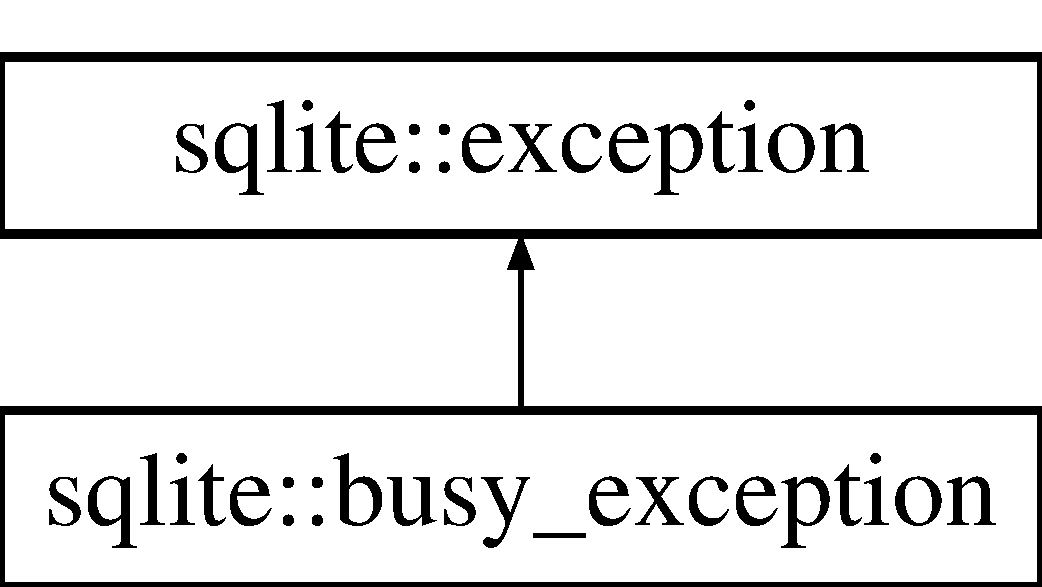
\includegraphics[height=2.000000cm]{a00003}
\end{center}
\end{figure}


\subsection{Detailed Description}
Encapsulation of the error code and message from S\-Q\-Lite3, based on std\-::runtime\-\_\-error. 



Definition at line 12 of file Exception.\-h.



The documentation for this class was generated from the following file\-:\begin{DoxyCompactItemize}
\item 
src/Exception.\-h\end{DoxyCompactItemize}

\hypertarget{a00004}{\section{sqlite\-:\-:dbconnection Class Reference}
\label{a00004}\index{sqlite\-::dbconnection@{sqlite\-::dbconnection}}
}


Class that represents a connection to a database.  




{\ttfamily \#include $<$D\-B\-Connection.\-h$>$}

\subsection*{Public Member Functions}
\begin{DoxyCompactItemize}
\item 
\hypertarget{a00004_a1cfe02390c4b08e78787120edaed6ab7}{\hyperlink{a00004_a1cfe02390c4b08e78787120edaed6ab7}{dbconnection} () noexcept}\label{a00004_a1cfe02390c4b08e78787120edaed6ab7}

\begin{DoxyCompactList}\small\item\em Default constructor. \end{DoxyCompactList}\item 
\hyperlink{a00004_a6c17517eb1631c15b64a0c54dd5355ca}{dbconnection} (const \hyperlink{a00004}{dbconnection} \&other) noexcept
\begin{DoxyCompactList}\small\item\em Copy constructor. \end{DoxyCompactList}\item 
\hyperlink{a00004_a31b78d1afbfc6147319eabb9f0e23bc5}{dbconnection} (\hyperlink{a00004}{dbconnection} \&\&other) noexcept
\begin{DoxyCompactList}\small\item\em Copy constructor. \end{DoxyCompactList}\item 
\hyperlink{a00004_a65e20f08669b49b018614cddd47efa77}{dbconnection} (const std\-::string \&filename, openmode mode=openmode\-::read\-\_\-write$\vert$openmode\-::create, const std\-::chrono\-::milliseconds timeout=D\-E\-F\-A\-U\-L\-T\-\_\-\-T\-I\-M\-E\-O\-U\-T)
\begin{DoxyCompactList}\small\item\em Open the provided database U\-T\-F-\/8 filename. \end{DoxyCompactList}\item 
\hyperlink{a00004_a4de544133c1a430855624c94986ed16c}{dbconnection} (const std\-::string \&filename, const std\-::chrono\-::milliseconds timeout)
\begin{DoxyCompactList}\small\item\em Open the provided database U\-T\-F-\/8 filename. \end{DoxyCompactList}\item 
\hyperlink{a00004_a1ac3a4126d0c5da0773f14e9ac443678}{dbconnection} (const std\-::u16string \&filename, const std\-::chrono\-::milliseconds timeout=D\-E\-F\-A\-U\-L\-T\-\_\-\-T\-I\-M\-E\-O\-U\-T)
\begin{DoxyCompactList}\small\item\em Open the provided database U\-T\-F-\/16 filename. \end{DoxyCompactList}\item 
\hyperlink{a00004}{dbconnection} \& \hyperlink{a00004_ae7c52ec41d3dfb7f4c8a521af7673bde}{operator=} (const \hyperlink{a00004}{dbconnection} \&other) noexcept
\begin{DoxyCompactList}\small\item\em Copy assignment operator. \end{DoxyCompactList}\item 
\hyperlink{a00004}{dbconnection} \& \hyperlink{a00004_abd91c727842023d54fdb64e6e2e9ac3c}{operator=} (\hyperlink{a00004}{dbconnection} \&\&other) noexcept
\begin{DoxyCompactList}\small\item\em Move assignment operator. \end{DoxyCompactList}\item 
\hyperlink{a00009}{sqlite\-::mutex} \hyperlink{a00004_afa13431e657c74ba7beee63fa70eeb93}{mutex} ()
\begin{DoxyCompactList}\small\item\em Returns a mutex that serializes access to the database. \end{DoxyCompactList}\item 
\hyperlink{a00004_a8c0e145b3687659ec0f76949174651e0}{operator bool} () const noexcept
\begin{DoxyCompactList}\small\item\em Specifies if the dbconnection has a open database connection. \end{DoxyCompactList}\item 
\hypertarget{a00004_a1a9b022293133991f265c10c1f50800b}{sqlite3 $\ast$ \hyperlink{a00004_a1a9b022293133991f265c10c1f50800b}{handle} () const noexcept}\label{a00004_a1a9b022293133991f265c10c1f50800b}

\begin{DoxyCompactList}\small\item\em Returns pointer to the underlying \char`\"{}sqlite3\char`\"{} object. \end{DoxyCompactList}\item 
void \hyperlink{a00004_a84da73c4ff1b162624da3e252c2a86c8}{open} (const std\-::string \&filename, openmode mode=openmode\-::read\-\_\-write$\vert$openmode\-::create)
\begin{DoxyCompactList}\small\item\em Open an \hyperlink{a00038}{S\-Q\-Lite} database file as specified by the filename argument. \end{DoxyCompactList}\item 
void \hyperlink{a00004_ac31065d17d9cbe1e1b3021bf11ff0229}{open} (const std\-::u16string \&filename)
\begin{DoxyCompactList}\small\item\em Open an \hyperlink{a00038}{S\-Q\-Lite} database file as specified by the filname argument. \end{DoxyCompactList}\item 
long long \hyperlink{a00004_add860c9b2c630bcfc178e3a7e878ea1b}{row\-\_\-id} () const noexcept
\begin{DoxyCompactList}\small\item\em Returns the rowid of the most recent successful \char`\"{}\-I\-N\-S\-E\-R\-T\char`\"{} into a rowid table or virtual table on database connection. \end{DoxyCompactList}\item 
{\footnotesize template$<$typename F $>$ }\\void \hyperlink{a00004_a3cc15c8f2784e6b706a5992c8014c2dd}{create\-\_\-general\-\_\-function} (const std\-::string \&name, F \&\&function, int is\-\_\-deterministic=false, const textencoding encoding=textencoding\-::utf8, int nargs=-\/1)
\begin{DoxyCompactList}\small\item\em Used to add S\-Q\-L functions or redefine the behavior of existing S\-Q\-L functions. \end{DoxyCompactList}\item 
{\footnotesize template$<$typename F $>$ }\\void \hyperlink{a00004_ad42c081096ec64f35710aa021f2f4b56}{create\-\_\-function} (const std\-::string \&name, F \&\&function, bool is\-\_\-deterministic=false, const textencoding encoding=textencoding\-::utf8)
\begin{DoxyCompactList}\small\item\em Used to add S\-Q\-L functions or redefine the behavior of existing S\-Q\-L functions. \end{DoxyCompactList}\item 
{\footnotesize template$<$typename A $>$ }\\void \hyperlink{a00004_ab3e54d1eef4c27734e45a61d27be386b}{create\-\_\-aggregate} (const std\-::string \&name, bool is\-\_\-deterministic=false, const textencoding encoding=textencoding\-::utf8)
\begin{DoxyCompactList}\small\item\em Used to add S\-Q\-L aggregate functions or redefine the behavior of existing S\-Q\-L aggregate functions. \end{DoxyCompactList}\item 
{\footnotesize template$<$typename F $>$ }\\void \hyperlink{a00004_ab8c7b939c1b6d41259aefa3b7475f3bd}{create\-\_\-collation} (const std\-::string \&name, F \&\&function, const textencoding encoding=textencoding\-::utf8)
\begin{DoxyCompactList}\small\item\em Used to add an S\-Q\-L collation or redefine the behavior of existing S\-Q\-L collations. \end{DoxyCompactList}\end{DoxyCompactItemize}
\subsection*{Static Public Member Functions}
\begin{DoxyCompactItemize}
\item 
static \hyperlink{a00004}{dbconnection} \hyperlink{a00004_adc0120a0d5d39eabcffb7d641b0c40dd}{memory} ()
\begin{DoxyCompactList}\small\item\em Create a purely in memory database. \end{DoxyCompactList}\item 
static \hyperlink{a00004}{dbconnection} \hyperlink{a00004_abe5e2bf211f18f2f358f4293d3064679}{wide\-\_\-memory} ()
\begin{DoxyCompactList}\small\item\em Create a purely in memory database with U\-T\-F-\/16 as the native byte order. \end{DoxyCompactList}\end{DoxyCompactItemize}


\subsection{Detailed Description}
Class that represents a connection to a database. 

The class dbconnection is a wrapper around the \char`\"{}sqlite3\char`\"{} structure. 

Definition at line 24 of file D\-B\-Connection.\-h.



\subsection{Constructor \& Destructor Documentation}
\hypertarget{a00004_a6c17517eb1631c15b64a0c54dd5355ca}{\index{sqlite\-::dbconnection@{sqlite\-::dbconnection}!dbconnection@{dbconnection}}
\index{dbconnection@{dbconnection}!sqlite::dbconnection@{sqlite\-::dbconnection}}
\subsubsection[{dbconnection}]{\setlength{\rightskip}{0pt plus 5cm}sqlite\-::dbconnection\-::dbconnection (
\begin{DoxyParamCaption}
\item[{const {\bf dbconnection} \&}]{other}
\end{DoxyParamCaption}
)\hspace{0.3cm}{\ttfamily [noexcept]}}}\label{a00004_a6c17517eb1631c15b64a0c54dd5355ca}


Copy constructor. 


\begin{DoxyParams}[1]{Parameters}
\mbox{\tt in}  & {\em other} & another dbconnection object to use as source to initialize object with. \\
\hline
\end{DoxyParams}


Definition at line 11 of file D\-B\-Connection.\-cpp.

\hypertarget{a00004_a31b78d1afbfc6147319eabb9f0e23bc5}{\index{sqlite\-::dbconnection@{sqlite\-::dbconnection}!dbconnection@{dbconnection}}
\index{dbconnection@{dbconnection}!sqlite::dbconnection@{sqlite\-::dbconnection}}
\subsubsection[{dbconnection}]{\setlength{\rightskip}{0pt plus 5cm}sqlite\-::dbconnection\-::dbconnection (
\begin{DoxyParamCaption}
\item[{{\bf dbconnection} \&\&}]{other}
\end{DoxyParamCaption}
)\hspace{0.3cm}{\ttfamily [noexcept]}}}\label{a00004_a31b78d1afbfc6147319eabb9f0e23bc5}


Copy constructor. 

Constructs a dbconnection object with a copy of the contents of other using move semantics. 
\begin{DoxyParams}[1]{Parameters}
\mbox{\tt in}  & {\em other} & another dbconnection object to use as source to initialize object with. \\
\hline
\end{DoxyParams}


Definition at line 15 of file D\-B\-Connection.\-cpp.

\hypertarget{a00004_a65e20f08669b49b018614cddd47efa77}{\index{sqlite\-::dbconnection@{sqlite\-::dbconnection}!dbconnection@{dbconnection}}
\index{dbconnection@{dbconnection}!sqlite::dbconnection@{sqlite\-::dbconnection}}
\subsubsection[{dbconnection}]{\setlength{\rightskip}{0pt plus 5cm}sqlite\-::dbconnection\-::dbconnection (
\begin{DoxyParamCaption}
\item[{const std\-::string \&}]{filename, }
\item[{openmode}]{mode = {\ttfamily openmode\-:\-:read\-\_\-write~$\vert$~openmode\-:\-:create}, }
\item[{const std\-::chrono\-::milliseconds}]{timeout = {\ttfamily DEFAULT\-\_\-TIMEOUT}}
\end{DoxyParamCaption}
)}}\label{a00004_a65e20f08669b49b018614cddd47efa77}


Open the provided database U\-T\-F-\/8 filename. 


\begin{DoxyParams}[1]{Parameters}
\mbox{\tt in}  & {\em filename} & U\-T\-F-\/8 path/uri to the database database file \\
\hline
\mbox{\tt in}  & {\em mode} & file opening options specified by combination of openmode flags \\
\hline
\mbox{\tt in}  & {\em timeout} & amount of milliseconds to wait before returning \hyperlink{a00003}{sqlite\-::busy\-\_\-exception} when a table is locked \\
\hline
\end{DoxyParams}


Definition at line 35 of file D\-B\-Connection.\-cpp.

\hypertarget{a00004_a4de544133c1a430855624c94986ed16c}{\index{sqlite\-::dbconnection@{sqlite\-::dbconnection}!dbconnection@{dbconnection}}
\index{dbconnection@{dbconnection}!sqlite::dbconnection@{sqlite\-::dbconnection}}
\subsubsection[{dbconnection}]{\setlength{\rightskip}{0pt plus 5cm}sqlite\-::dbconnection\-::dbconnection (
\begin{DoxyParamCaption}
\item[{const std\-::string \&}]{filename, }
\item[{const std\-::chrono\-::milliseconds}]{timeout}
\end{DoxyParamCaption}
)}}\label{a00004_a4de544133c1a430855624c94986ed16c}


Open the provided database U\-T\-F-\/8 filename. 


\begin{DoxyParams}[1]{Parameters}
\mbox{\tt in}  & {\em filename} & U\-T\-F-\/8 path/uri to the database database file \\
\hline
\mbox{\tt in}  & {\em timeout} & amount of milliseconds to wait before returning \hyperlink{a00003}{sqlite\-::busy\-\_\-exception} when a table is locked \\
\hline
\end{DoxyParams}


Definition at line 44 of file D\-B\-Connection.\-cpp.

\hypertarget{a00004_a1ac3a4126d0c5da0773f14e9ac443678}{\index{sqlite\-::dbconnection@{sqlite\-::dbconnection}!dbconnection@{dbconnection}}
\index{dbconnection@{dbconnection}!sqlite::dbconnection@{sqlite\-::dbconnection}}
\subsubsection[{dbconnection}]{\setlength{\rightskip}{0pt plus 5cm}sqlite\-::dbconnection\-::dbconnection (
\begin{DoxyParamCaption}
\item[{const std\-::u16string \&}]{filename, }
\item[{const std\-::chrono\-::milliseconds}]{timeout = {\ttfamily DEFAULT\-\_\-TIMEOUT}}
\end{DoxyParamCaption}
)}}\label{a00004_a1ac3a4126d0c5da0773f14e9ac443678}


Open the provided database U\-T\-F-\/16 filename. 


\begin{DoxyParams}[1]{Parameters}
\mbox{\tt in}  & {\em filename} & U\-T\-F-\/16 path/uri to the database database file \\
\hline
\mbox{\tt in}  & {\em timeout} & Amount of milliseconds to wait before returning \hyperlink{a00003}{sqlite\-::busy\-\_\-exception} when a table is locked \\
\hline
\end{DoxyParams}


Definition at line 52 of file D\-B\-Connection.\-cpp.



\subsection{Member Function Documentation}
\hypertarget{a00004_ab3e54d1eef4c27734e45a61d27be386b}{\index{sqlite\-::dbconnection@{sqlite\-::dbconnection}!create\-\_\-aggregate@{create\-\_\-aggregate}}
\index{create\-\_\-aggregate@{create\-\_\-aggregate}!sqlite::dbconnection@{sqlite\-::dbconnection}}
\subsubsection[{create\-\_\-aggregate}]{\setlength{\rightskip}{0pt plus 5cm}template$<$typename A $>$ void sqlite\-::dbconnection\-::create\-\_\-aggregate (
\begin{DoxyParamCaption}
\item[{const std\-::string \&}]{name, }
\item[{bool}]{is\-\_\-deterministic = {\ttfamily false}, }
\item[{const textencoding}]{encoding = {\ttfamily textencoding\-:\-:utf8}}
\end{DoxyParamCaption}
)\hspace{0.3cm}{\ttfamily [inline]}}}\label{a00004_ab3e54d1eef4c27734e45a61d27be386b}


Used to add S\-Q\-L aggregate functions or redefine the behavior of existing S\-Q\-L aggregate functions. 


\begin{DoxyTemplParams}{Template Parameters}
{\em A} & The class to use as the aggregate function. \\
\hline
\end{DoxyTemplParams}

\begin{DoxyParams}[1]{Parameters}
\mbox{\tt in}  & {\em name} & the name of the aggregate function to be used in an S\-Q\-L query \\
\hline
\mbox{\tt in}  & {\em is\-\_\-deterministic} & specifies if the function will always return the same result given the same inputs within a single S\-Q\-L statement. \\
\hline
\mbox{\tt in}  & {\em encoding} & specifies the test encoding the S\-Q\-L function prefers for its parameters \\
\hline
\end{DoxyParams}


Definition at line 203 of file D\-B\-Connection.\-h.

\hypertarget{a00004_ab8c7b939c1b6d41259aefa3b7475f3bd}{\index{sqlite\-::dbconnection@{sqlite\-::dbconnection}!create\-\_\-collation@{create\-\_\-collation}}
\index{create\-\_\-collation@{create\-\_\-collation}!sqlite::dbconnection@{sqlite\-::dbconnection}}
\subsubsection[{create\-\_\-collation}]{\setlength{\rightskip}{0pt plus 5cm}template$<$typename F $>$ void sqlite\-::dbconnection\-::create\-\_\-collation (
\begin{DoxyParamCaption}
\item[{const std\-::string \&}]{name, }
\item[{F \&\&}]{function, }
\item[{const textencoding}]{encoding = {\ttfamily textencoding\-:\-:utf8}}
\end{DoxyParamCaption}
)\hspace{0.3cm}{\ttfamily [inline]}}}\label{a00004_ab8c7b939c1b6d41259aefa3b7475f3bd}


Used to add an S\-Q\-L collation or redefine the behavior of existing S\-Q\-L collations. 


\begin{DoxyTemplParams}{Template Parameters}
{\em F} & The function type to use to create the function. \\
\hline
\end{DoxyTemplParams}

\begin{DoxyParams}[1]{Parameters}
\mbox{\tt in}  & {\em name} & the name of the function to be used in an S\-Q\-L query \\
\hline
\mbox{\tt in}  & {\em function} & the implementation to the function \\
\hline
\mbox{\tt in}  & {\em encoding} & specifies the test encoding the S\-Q\-L function prefers for its parameters \\
\hline
\end{DoxyParams}


Definition at line 237 of file D\-B\-Connection.\-h.

\hypertarget{a00004_ad42c081096ec64f35710aa021f2f4b56}{\index{sqlite\-::dbconnection@{sqlite\-::dbconnection}!create\-\_\-function@{create\-\_\-function}}
\index{create\-\_\-function@{create\-\_\-function}!sqlite::dbconnection@{sqlite\-::dbconnection}}
\subsubsection[{create\-\_\-function}]{\setlength{\rightskip}{0pt plus 5cm}template$<$typename F $>$ void sqlite\-::dbconnection\-::create\-\_\-function (
\begin{DoxyParamCaption}
\item[{const std\-::string \&}]{name, }
\item[{F \&\&}]{function, }
\item[{bool}]{is\-\_\-deterministic = {\ttfamily false}, }
\item[{const textencoding}]{encoding = {\ttfamily textencoding\-:\-:utf8}}
\end{DoxyParamCaption}
)\hspace{0.3cm}{\ttfamily [inline]}}}\label{a00004_ad42c081096ec64f35710aa021f2f4b56}


Used to add S\-Q\-L functions or redefine the behavior of existing S\-Q\-L functions. 


\begin{DoxyTemplParams}{Template Parameters}
{\em F} & The function type to use to create the function. \\
\hline
\end{DoxyTemplParams}

\begin{DoxyParams}[1]{Parameters}
\mbox{\tt in}  & {\em name} & the name of the function to be used in an S\-Q\-L query \\
\hline
\mbox{\tt in}  & {\em function} & the implementation to the function \\
\hline
\mbox{\tt in}  & {\em is\-\_\-deterministic} & specifies if the function will always return the same result given the same inputs within a single S\-Q\-L statement. \\
\hline
\mbox{\tt in}  & {\em encoding} & specifies the test encoding the S\-Q\-L function prefers for its parameters \\
\hline
\end{DoxyParams}


Definition at line 168 of file D\-B\-Connection.\-h.

\hypertarget{a00004_a3cc15c8f2784e6b706a5992c8014c2dd}{\index{sqlite\-::dbconnection@{sqlite\-::dbconnection}!create\-\_\-general\-\_\-function@{create\-\_\-general\-\_\-function}}
\index{create\-\_\-general\-\_\-function@{create\-\_\-general\-\_\-function}!sqlite::dbconnection@{sqlite\-::dbconnection}}
\subsubsection[{create\-\_\-general\-\_\-function}]{\setlength{\rightskip}{0pt plus 5cm}template$<$typename F $>$ void sqlite\-::dbconnection\-::create\-\_\-general\-\_\-function (
\begin{DoxyParamCaption}
\item[{const std\-::string \&}]{name, }
\item[{F \&\&}]{function, }
\item[{int}]{is\-\_\-deterministic = {\ttfamily false}, }
\item[{const textencoding}]{encoding = {\ttfamily textencoding\-:\-:utf8}, }
\item[{int}]{nargs = {\ttfamily -\/1}}
\end{DoxyParamCaption}
)\hspace{0.3cm}{\ttfamily [inline]}}}\label{a00004_a3cc15c8f2784e6b706a5992c8014c2dd}


Used to add S\-Q\-L functions or redefine the behavior of existing S\-Q\-L functions. 


\begin{DoxyTemplParams}{Template Parameters}
{\em F} & The function type to use to create the function. \\
\hline
\end{DoxyTemplParams}

\begin{DoxyParams}[1]{Parameters}
\mbox{\tt in}  & {\em name} & the name of the function to be used in an S\-Q\-L query \\
\hline
\mbox{\tt in}  & {\em function} & the implementation to the function \\
\hline
\mbox{\tt in}  & {\em is\-\_\-deterministic} & specifies if the function will always return the same result given the same inputs within a single S\-Q\-L statement. \\
\hline
\mbox{\tt in}  & {\em encoding} & specifies the text encoding the S\-Q\-L function prefers for its parameters. \\
\hline
\mbox{\tt in}  & {\em nargs} & the number of arguments that the S\-Q\-L function takes. -\/1 means the S\-Q\-L function can take any number of arguments. \\
\hline
\end{DoxyParams}


Definition at line 131 of file D\-B\-Connection.\-h.

\hypertarget{a00004_adc0120a0d5d39eabcffb7d641b0c40dd}{\index{sqlite\-::dbconnection@{sqlite\-::dbconnection}!memory@{memory}}
\index{memory@{memory}!sqlite::dbconnection@{sqlite\-::dbconnection}}
\subsubsection[{memory}]{\setlength{\rightskip}{0pt plus 5cm}{\bf dbconnection} sqlite\-::dbconnection\-::memory (
\begin{DoxyParamCaption}
{}
\end{DoxyParamCaption}
)\hspace{0.3cm}{\ttfamily [static]}}}\label{a00004_adc0120a0d5d39eabcffb7d641b0c40dd}


Create a purely in memory database. 

\begin{DoxyReturn}{Returns}
a purely in memory \hyperlink{a00004}{sqlite\-::dbconnection} 
\end{DoxyReturn}


Definition at line 60 of file D\-B\-Connection.\-cpp.

\hypertarget{a00004_afa13431e657c74ba7beee63fa70eeb93}{\index{sqlite\-::dbconnection@{sqlite\-::dbconnection}!mutex@{mutex}}
\index{mutex@{mutex}!sqlite::dbconnection@{sqlite\-::dbconnection}}
\subsubsection[{mutex}]{\setlength{\rightskip}{0pt plus 5cm}{\bf mutex} sqlite\-::dbconnection\-::mutex (
\begin{DoxyParamCaption}
{}
\end{DoxyParamCaption}
)}}\label{a00004_afa13431e657c74ba7beee63fa70eeb93}


Returns a mutex that serializes access to the database. 

\begin{DoxyReturn}{Returns}
A mutex object for the database connection. 
\end{DoxyReturn}


Definition at line 70 of file D\-B\-Connection.\-cpp.

\hypertarget{a00004_a84da73c4ff1b162624da3e252c2a86c8}{\index{sqlite\-::dbconnection@{sqlite\-::dbconnection}!open@{open}}
\index{open@{open}!sqlite::dbconnection@{sqlite\-::dbconnection}}
\subsubsection[{open}]{\setlength{\rightskip}{0pt plus 5cm}void sqlite\-::dbconnection\-::open (
\begin{DoxyParamCaption}
\item[{const std\-::string \&}]{filename, }
\item[{openmode}]{mode = {\ttfamily openmode\-:\-:read\-\_\-write~$\vert$~openmode\-:\-:create}}
\end{DoxyParamCaption}
)}}\label{a00004_a84da73c4ff1b162624da3e252c2a86c8}


Open an \hyperlink{a00038}{S\-Q\-Lite} database file as specified by the filename argument. 


\begin{DoxyParams}[1]{Parameters}
\mbox{\tt in}  & {\em filename} & path to \hyperlink{a00038}{S\-Q\-Lite} file \\
\hline
\mbox{\tt in}  & {\em mode} & specifies the privileges to use when opening the database. \\
\hline
\end{DoxyParams}


Definition at line 89 of file D\-B\-Connection.\-cpp.

\hypertarget{a00004_ac31065d17d9cbe1e1b3021bf11ff0229}{\index{sqlite\-::dbconnection@{sqlite\-::dbconnection}!open@{open}}
\index{open@{open}!sqlite::dbconnection@{sqlite\-::dbconnection}}
\subsubsection[{open}]{\setlength{\rightskip}{0pt plus 5cm}void sqlite\-::dbconnection\-::open (
\begin{DoxyParamCaption}
\item[{const std\-::u16string \&}]{filename}
\end{DoxyParamCaption}
)}}\label{a00004_ac31065d17d9cbe1e1b3021bf11ff0229}


Open an \hyperlink{a00038}{S\-Q\-Lite} database file as specified by the filname argument. 

The database file will have U\-T\-F-\/16 native byte order. 
\begin{DoxyParams}[1]{Parameters}
\mbox{\tt in}  & {\em filename} & path to \hyperlink{a00038}{S\-Q\-Lite} file \\
\hline
\end{DoxyParams}


Definition at line 101 of file D\-B\-Connection.\-cpp.

\hypertarget{a00004_a8c0e145b3687659ec0f76949174651e0}{\index{sqlite\-::dbconnection@{sqlite\-::dbconnection}!operator bool@{operator bool}}
\index{operator bool@{operator bool}!sqlite::dbconnection@{sqlite\-::dbconnection}}
\subsubsection[{operator bool}]{\setlength{\rightskip}{0pt plus 5cm}sqlite\-::dbconnection\-::operator bool (
\begin{DoxyParamCaption}
{}
\end{DoxyParamCaption}
) const\hspace{0.3cm}{\ttfamily [explicit]}, {\ttfamily [noexcept]}}}\label{a00004_a8c0e145b3687659ec0f76949174651e0}


Specifies if the dbconnection has a open database connection. 

\begin{DoxyReturn}{Returns}
Returns true if the dbconnection has a open database connection associated associated with it. 
\end{DoxyReturn}


Definition at line 79 of file D\-B\-Connection.\-cpp.

\hypertarget{a00004_ae7c52ec41d3dfb7f4c8a521af7673bde}{\index{sqlite\-::dbconnection@{sqlite\-::dbconnection}!operator=@{operator=}}
\index{operator=@{operator=}!sqlite::dbconnection@{sqlite\-::dbconnection}}
\subsubsection[{operator=}]{\setlength{\rightskip}{0pt plus 5cm}{\bf dbconnection} \& sqlite\-::dbconnection\-::operator= (
\begin{DoxyParamCaption}
\item[{const {\bf dbconnection} \&}]{other}
\end{DoxyParamCaption}
)\hspace{0.3cm}{\ttfamily [noexcept]}}}\label{a00004_ae7c52ec41d3dfb7f4c8a521af7673bde}


Copy assignment operator. 

Replaces the contents with those of other. 
\begin{DoxyParams}[1]{Parameters}
\mbox{\tt in}  & {\em other} & another dbconnection object to use as source to initialize object with. \\
\hline
\end{DoxyParams}
\begin{DoxyReturn}{Returns}
$\ast$this 
\end{DoxyReturn}


Definition at line 19 of file D\-B\-Connection.\-cpp.

\hypertarget{a00004_abd91c727842023d54fdb64e6e2e9ac3c}{\index{sqlite\-::dbconnection@{sqlite\-::dbconnection}!operator=@{operator=}}
\index{operator=@{operator=}!sqlite::dbconnection@{sqlite\-::dbconnection}}
\subsubsection[{operator=}]{\setlength{\rightskip}{0pt plus 5cm}{\bf dbconnection} \& sqlite\-::dbconnection\-::operator= (
\begin{DoxyParamCaption}
\item[{{\bf dbconnection} \&\&}]{other}
\end{DoxyParamCaption}
)\hspace{0.3cm}{\ttfamily [noexcept]}}}\label{a00004_abd91c727842023d54fdb64e6e2e9ac3c}


Move assignment operator. 

Replaces the contents with those of other using move semantics. 
\begin{DoxyParams}[1]{Parameters}
\mbox{\tt in}  & {\em other} & another dbconnection object to use as source to initialize object with. \\
\hline
\end{DoxyParams}
\begin{DoxyReturn}{Returns}
$\ast$this 
\end{DoxyReturn}


Definition at line 28 of file D\-B\-Connection.\-cpp.

\hypertarget{a00004_add860c9b2c630bcfc178e3a7e878ea1b}{\index{sqlite\-::dbconnection@{sqlite\-::dbconnection}!row\-\_\-id@{row\-\_\-id}}
\index{row\-\_\-id@{row\-\_\-id}!sqlite::dbconnection@{sqlite\-::dbconnection}}
\subsubsection[{row\-\_\-id}]{\setlength{\rightskip}{0pt plus 5cm}long long sqlite\-::dbconnection\-::row\-\_\-id (
\begin{DoxyParamCaption}
{}
\end{DoxyParamCaption}
) const\hspace{0.3cm}{\ttfamily [noexcept]}}}\label{a00004_add860c9b2c630bcfc178e3a7e878ea1b}


Returns the rowid of the most recent successful \char`\"{}\-I\-N\-S\-E\-R\-T\char`\"{} into a rowid table or virtual table on database connection. 

\begin{DoxyReturn}{Returns}
rowid of the most recent successful \char`\"{}\-I\-N\-S\-E\-R\-T\char`\"{} into the database, or 0 if there was none. 
\end{DoxyReturn}


Definition at line 113 of file D\-B\-Connection.\-cpp.

\hypertarget{a00004_abe5e2bf211f18f2f358f4293d3064679}{\index{sqlite\-::dbconnection@{sqlite\-::dbconnection}!wide\-\_\-memory@{wide\-\_\-memory}}
\index{wide\-\_\-memory@{wide\-\_\-memory}!sqlite::dbconnection@{sqlite\-::dbconnection}}
\subsubsection[{wide\-\_\-memory}]{\setlength{\rightskip}{0pt plus 5cm}{\bf dbconnection} sqlite\-::dbconnection\-::wide\-\_\-memory (
\begin{DoxyParamCaption}
{}
\end{DoxyParamCaption}
)\hspace{0.3cm}{\ttfamily [static]}}}\label{a00004_abe5e2bf211f18f2f358f4293d3064679}


Create a purely in memory database with U\-T\-F-\/16 as the native byte order. 

\begin{DoxyReturn}{Returns}
a purely in memory \hyperlink{a00004}{sqlite\-::dbconnection} 
\end{DoxyReturn}


Definition at line 65 of file D\-B\-Connection.\-cpp.



The documentation for this class was generated from the following files\-:\begin{DoxyCompactItemize}
\item 
src/\hyperlink{a00022}{D\-B\-Connection.\-h}\item 
src/D\-B\-Connection.\-cpp\end{DoxyCompactItemize}

\hypertarget{a00005}{\section{S\-Q\-Lite\-:\-:Mutex Class Reference}
\label{a00005}\index{S\-Q\-Lite\-::\-Mutex@{S\-Q\-Lite\-::\-Mutex}}
}


Helps with serializing access to a database connection.  




{\ttfamily \#include $<$Mutex.\-h$>$}

\subsection*{Public Member Functions}
\begin{DoxyCompactItemize}
\item 
\hypertarget{a00005_a56ba1f0c1411940ab52279497d15812a}{void \hyperlink{a00005_a56ba1f0c1411940ab52279497d15812a}{lock} () noexcept}\label{a00005_a56ba1f0c1411940ab52279497d15812a}

\begin{DoxyCompactList}\small\item\em Locks the mutex, blocks if the mutex is not available. \end{DoxyCompactList}\item 
bool \hyperlink{a00005_a95b5ebd5fef0bd37b30e3867d60389f8}{try\-Lock} () noexcept
\begin{DoxyCompactList}\small\item\em Tries to lock the mutex, returns if the mutex is not available. \end{DoxyCompactList}\item 
\hypertarget{a00005_ad9238aeb94205ac18d67c9652dcc6ef9}{void \hyperlink{a00005_ad9238aeb94205ac18d67c9652dcc6ef9}{unlock} () noexcept}\label{a00005_ad9238aeb94205ac18d67c9652dcc6ef9}

\begin{DoxyCompactList}\small\item\em Unlocks the mutex. \end{DoxyCompactList}\end{DoxyCompactItemize}


\subsection{Detailed Description}
Helps with serializing access to a database connection. 

Mutexes are only useful when threading mode is set to \char`\"{}\-Serialized\char`\"{}. 

Definition at line 12 of file Mutex.\-h.



\subsection{Member Function Documentation}
\hypertarget{a00005_a95b5ebd5fef0bd37b30e3867d60389f8}{\index{S\-Q\-Lite\-::\-Mutex@{S\-Q\-Lite\-::\-Mutex}!try\-Lock@{try\-Lock}}
\index{try\-Lock@{try\-Lock}!SQLite::Mutex@{S\-Q\-Lite\-::\-Mutex}}
\subsubsection[{try\-Lock}]{\setlength{\rightskip}{0pt plus 5cm}bool S\-Q\-Lite\-::\-Mutex\-::try\-Lock (
\begin{DoxyParamCaption}
{}
\end{DoxyParamCaption}
)\hspace{0.3cm}{\ttfamily [noexcept]}}}\label{a00005_a95b5ebd5fef0bd37b30e3867d60389f8}


Tries to lock the mutex, returns if the mutex is not available. 

\begin{DoxyReturn}{Returns}
True if able to obtain lock. False otherwise. 
\end{DoxyReturn}


Definition at line 22 of file Mutex.\-cpp.



The documentation for this class was generated from the following files\-:\begin{DoxyCompactItemize}
\item 
src/Mutex.\-h\item 
src/Mutex.\-cpp\end{DoxyCompactItemize}

\hypertarget{a00006}{\section{sqlite\-:\-:exception Class Reference}
\label{a00006}\index{sqlite\-::exception@{sqlite\-::exception}}
}


Encapsulation of the error code and message from S\-Q\-Lite3, based on std\-::runtime\-\_\-error.  




{\ttfamily \#include $<$Exception.\-h$>$}

Inheritance diagram for sqlite\-:\-:exception\-:\begin{figure}[H]
\begin{center}
\leavevmode
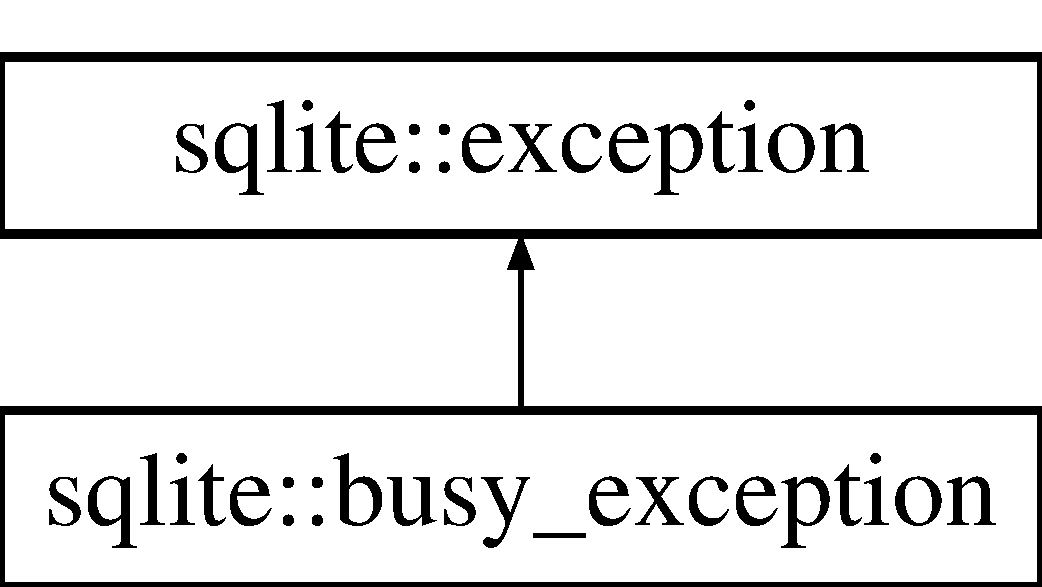
\includegraphics[height=2.000000cm]{a00006}
\end{center}
\end{figure}


\subsection{Detailed Description}
Encapsulation of the error code and message from S\-Q\-Lite3, based on std\-::runtime\-\_\-error. 



Definition at line 14 of file Exception.\-h.



The documentation for this class was generated from the following file\-:\begin{DoxyCompactItemize}
\item 
src/\hyperlink{a00024}{Exception.\-h}\end{DoxyCompactItemize}

\hypertarget{a00007}{\section{S\-Q\-Lite\-:\-:Exclusive\-Transaction Class Reference}
\label{a00007}\index{S\-Q\-Lite\-::\-Exclusive\-Transaction@{S\-Q\-Lite\-::\-Exclusive\-Transaction}}
}


R\-A\-I\-I encapsulation of the \hyperlink{a00038}{S\-Q\-Lite} exclusive transaction.  




{\ttfamily \#include $<$Transaction.\-h$>$}

Inheritance diagram for S\-Q\-Lite\-:\-:Exclusive\-Transaction\-:\begin{figure}[H]
\begin{center}
\leavevmode
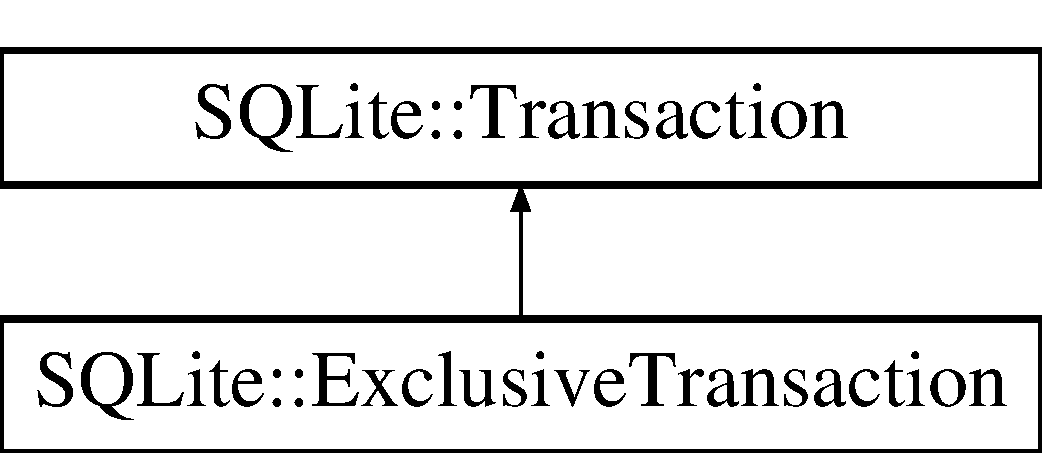
\includegraphics[height=2.000000cm]{a00007}
\end{center}
\end{figure}
\subsection*{Public Member Functions}
\begin{DoxyCompactItemize}
\item 
\hyperlink{a00007_a70f16f1e9764fd35b0c7e9fbf7314a1f}{Exclusive\-Transaction} (\hyperlink{a00004}{D\-B\-Connection} \&connection)
\begin{DoxyCompactList}\small\item\em Implements a strictly scope-\/based \hyperlink{a00038}{S\-Q\-Lite} exclusive transaction. \end{DoxyCompactList}\item 
\hypertarget{a00014_a9b251d84198cdc2c0208ad566fec0287}{virtual void \hyperlink{a00014_a9b251d84198cdc2c0208ad566fec0287}{commit} ()}\label{a00014_a9b251d84198cdc2c0208ad566fec0287}

\begin{DoxyCompactList}\small\item\em Commit the transaction. \end{DoxyCompactList}\end{DoxyCompactItemize}


\subsection{Detailed Description}
R\-A\-I\-I encapsulation of the \hyperlink{a00038}{S\-Q\-Lite} exclusive transaction. 

Definition at line 83 of file Transaction.\-h.



\subsection{Constructor \& Destructor Documentation}
\hypertarget{a00007_a70f16f1e9764fd35b0c7e9fbf7314a1f}{\index{S\-Q\-Lite\-::\-Exclusive\-Transaction@{S\-Q\-Lite\-::\-Exclusive\-Transaction}!Exclusive\-Transaction@{Exclusive\-Transaction}}
\index{Exclusive\-Transaction@{Exclusive\-Transaction}!SQLite::ExclusiveTransaction@{S\-Q\-Lite\-::\-Exclusive\-Transaction}}
\subsubsection[{Exclusive\-Transaction}]{\setlength{\rightskip}{0pt plus 5cm}S\-Q\-Lite\-::\-Exclusive\-Transaction\-::\-Exclusive\-Transaction (
\begin{DoxyParamCaption}
\item[{{\bf D\-B\-Connection} \&}]{connection}
\end{DoxyParamCaption}
)\hspace{0.3cm}{\ttfamily [inline]}}}\label{a00007_a70f16f1e9764fd35b0c7e9fbf7314a1f}


Implements a strictly scope-\/based \hyperlink{a00038}{S\-Q\-Lite} exclusive transaction. 


\begin{DoxyParams}[1]{Parameters}
\mbox{\tt in}  & {\em connection} & the database connection to begin the transaction on \\
\hline
\end{DoxyParams}


Definition at line 89 of file Transaction.\-h.



The documentation for this class was generated from the following file\-:\begin{DoxyCompactItemize}
\item 
src/\hyperlink{a00034}{Transaction.\-h}\end{DoxyCompactItemize}

\hypertarget{a00008}{\section{sqlite\-:\-:immediate\-\_\-transaction Class Reference}
\label{a00008}\index{sqlite\-::immediate\-\_\-transaction@{sqlite\-::immediate\-\_\-transaction}}
}


R\-A\-I\-I encapsulation of the S\-Q\-Lite immediate transaction.  




{\ttfamily \#include $<$Transaction.\-h$>$}

Inheritance diagram for sqlite\-:\-:immediate\-\_\-transaction\-:\begin{figure}[H]
\begin{center}
\leavevmode
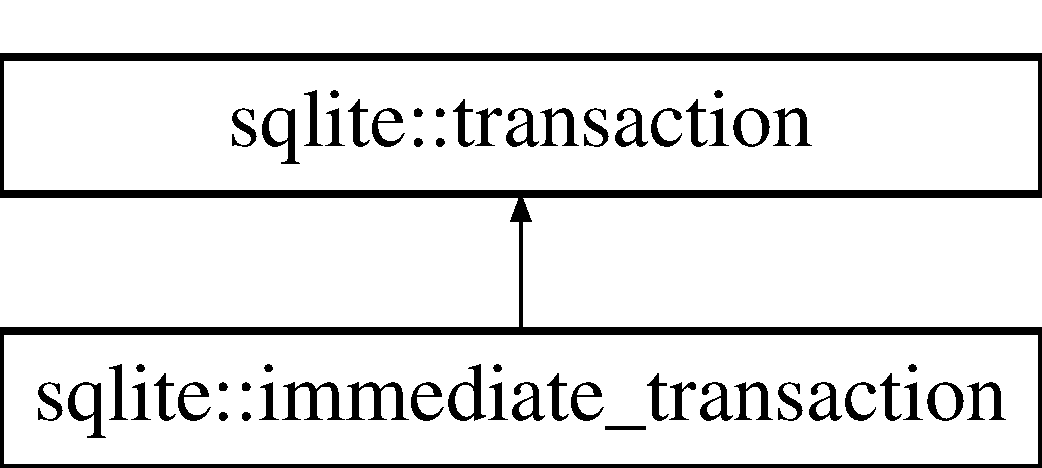
\includegraphics[height=2.000000cm]{a00008}
\end{center}
\end{figure}
\subsection*{Public Member Functions}
\begin{DoxyCompactItemize}
\item 
\hyperlink{a00008_a17924d6e15666b8340ee8aab9a88e0d1}{immediate\-\_\-transaction} (\hyperlink{a00004}{dbconnection} \&connection)
\begin{DoxyCompactList}\small\item\em Implements a strictly scope-\/based S\-Q\-Lite immediate transaction. \end{DoxyCompactList}\item 
\hypertarget{a00014_abe219dd0bf949d569381f9830c7b2d1a}{virtual void \hyperlink{a00014_abe219dd0bf949d569381f9830c7b2d1a}{commit} ()}\label{a00014_abe219dd0bf949d569381f9830c7b2d1a}

\begin{DoxyCompactList}\small\item\em Commit the transaction. \end{DoxyCompactList}\end{DoxyCompactItemize}


\subsection{Detailed Description}
R\-A\-I\-I encapsulation of the S\-Q\-Lite immediate transaction. 

Definition at line 70 of file Transaction.\-h.



\subsection{Constructor \& Destructor Documentation}
\hypertarget{a00008_a17924d6e15666b8340ee8aab9a88e0d1}{\index{sqlite\-::immediate\-\_\-transaction@{sqlite\-::immediate\-\_\-transaction}!immediate\-\_\-transaction@{immediate\-\_\-transaction}}
\index{immediate\-\_\-transaction@{immediate\-\_\-transaction}!sqlite::immediate_transaction@{sqlite\-::immediate\-\_\-transaction}}
\subsubsection[{immediate\-\_\-transaction}]{\setlength{\rightskip}{0pt plus 5cm}sqlite\-::immediate\-\_\-transaction\-::immediate\-\_\-transaction (
\begin{DoxyParamCaption}
\item[{{\bf dbconnection} \&}]{connection}
\end{DoxyParamCaption}
)\hspace{0.3cm}{\ttfamily [inline]}}}\label{a00008_a17924d6e15666b8340ee8aab9a88e0d1}


Implements a strictly scope-\/based S\-Q\-Lite immediate transaction. 


\begin{DoxyParams}[1]{Parameters}
\mbox{\tt in}  & {\em connection} & the database connection to begin the transaction on \\
\hline
\end{DoxyParams}


Definition at line 76 of file Transaction.\-h.



The documentation for this class was generated from the following file\-:\begin{DoxyCompactItemize}
\item 
src/\hyperlink{a00034}{Transaction.\-h}\end{DoxyCompactItemize}

\hypertarget{a00009}{\section{S\-Q\-Lite\-:\-:Transaction Class Reference}
\label{a00009}\index{S\-Q\-Lite\-::\-Transaction@{S\-Q\-Lite\-::\-Transaction}}
}


R\-A\-I\-I encapsulation of the S\-Q\-Lite Transactions.  




{\ttfamily \#include $<$Transaction.\-h$>$}



Inherited by S\-Q\-Lite\-::\-Deferred\-Transaction, S\-Q\-Lite\-::\-Exclusive\-Transaction, and S\-Q\-Lite\-::\-Immediate\-Transaction.

\subsection*{Public Member Functions}
\begin{DoxyCompactItemize}
\item 
\hyperlink{a00009_a27add1a1db2dd8cd5935c78a63ad556b}{Transaction} (\hyperlink{a00002}{D\-B\-Connection} \&connection, const Transaction\-Type type)
\begin{DoxyCompactList}\small\item\em Begins the S\-Q\-Lite transaction. \end{DoxyCompactList}\item 
\hypertarget{a00009_a43c5e67a10b9698b7f6dad73539feb94}{virtual \hyperlink{a00009_a43c5e67a10b9698b7f6dad73539feb94}{$\sim$\-Transaction} () noexcept}\label{a00009_a43c5e67a10b9698b7f6dad73539feb94}

\begin{DoxyCompactList}\small\item\em Safely rollback the transaction if it has not been commited. \end{DoxyCompactList}\item 
\hypertarget{a00009_a9b251d84198cdc2c0208ad566fec0287}{virtual void \hyperlink{a00009_a9b251d84198cdc2c0208ad566fec0287}{commit} ()}\label{a00009_a9b251d84198cdc2c0208ad566fec0287}

\begin{DoxyCompactList}\small\item\em Commit the transaction. \end{DoxyCompactList}\end{DoxyCompactItemize}


\subsection{Detailed Description}
R\-A\-I\-I encapsulation of the S\-Q\-Lite Transactions. 

Definition at line 21 of file Transaction.\-h.



\subsection{Constructor \& Destructor Documentation}
\hypertarget{a00009_a27add1a1db2dd8cd5935c78a63ad556b}{\index{S\-Q\-Lite\-::\-Transaction@{S\-Q\-Lite\-::\-Transaction}!Transaction@{Transaction}}
\index{Transaction@{Transaction}!SQLite::Transaction@{S\-Q\-Lite\-::\-Transaction}}
\subsubsection[{Transaction}]{\setlength{\rightskip}{0pt plus 5cm}S\-Q\-Lite\-::\-Transaction\-::\-Transaction (
\begin{DoxyParamCaption}
\item[{{\bf D\-B\-Connection} \&}]{connection, }
\item[{const Transaction\-Type}]{type}
\end{DoxyParamCaption}
)}}\label{a00009_a27add1a1db2dd8cd5935c78a63ad556b}


Begins the S\-Q\-Lite transaction. 


\begin{DoxyParams}[1]{Parameters}
\mbox{\tt in}  & {\em connection} & the database connection to begin the transaction on \\
\hline
\end{DoxyParams}


Definition at line 10 of file Transaction.\-cpp.



The documentation for this class was generated from the following files\-:\begin{DoxyCompactItemize}
\item 
src/Transaction.\-h\item 
src/Transaction.\-cpp\end{DoxyCompactItemize}

\hypertarget{a00010}{\section{S\-Q\-Lite\-:\-:Reader$<$ T $>$ Class Template Reference}
\label{a00010}\index{S\-Q\-Lite\-::\-Reader$<$ T $>$@{S\-Q\-Lite\-::\-Reader$<$ T $>$}}
}


Base class used to help with reading \char`\"{}sqlite3\-\_\-stmt\char`\"{} information.  




{\ttfamily \#include $<$Statement.\-h$>$}

\subsection*{Public Member Functions}
\begin{DoxyCompactItemize}
\item 
int \hyperlink{a00010_a82c5bc45048b8328a2fcc9bb4ff975f2}{get\-Int} (const int column) const noexcept
\begin{DoxyCompactList}\small\item\em Returns the specified column value as an integer. \end{DoxyCompactList}\item 
int \hyperlink{a00010_a87dd8234c2bd5f19466813f8a68ab80a}{get\-Int} (const std\-::string \&name) const noexcept
\begin{DoxyCompactList}\small\item\em Returns the specified column value as an integer. \end{DoxyCompactList}\item 
int64\-\_\-t \hyperlink{a00010_adb7b9705a4638d6d5af5ca26dfa474ff}{get\-Int64} (const int column) const noexcept
\begin{DoxyCompactList}\small\item\em Returns the specified column value as a 64-\/bit integer. \end{DoxyCompactList}\item 
int64\-\_\-t \hyperlink{a00010_aea6d24bb9247bfc52fe77d62be961dd2}{get\-Int64} (const std\-::string \&name) const noexcept
\begin{DoxyCompactList}\small\item\em Returns the specified column value as a 64-\/bit integer. \end{DoxyCompactList}\item 
unsigned int \hyperlink{a00010_a971fb706b9215a89532ac48640f94832}{get\-U\-Int} (const int column) const noexcept
\begin{DoxyCompactList}\small\item\em Returns the specified column value as an unsigned integer. \end{DoxyCompactList}\item 
unsigned int \hyperlink{a00010_a18315a8379249158c3f827441e8f6de0}{get\-U\-Int} (const std\-::string \&name) const noexcept
\begin{DoxyCompactList}\small\item\em Returns the specified column value as an unsigned integer. \end{DoxyCompactList}\item 
double \hyperlink{a00010_a679e56078c78e01c99fa08ad0b7ee782}{get\-Double} (const int column) const noexcept
\begin{DoxyCompactList}\small\item\em Returns the specified column value as a double. \end{DoxyCompactList}\item 
double \hyperlink{a00010_a45e9dd813439e8cda7608e18c1ccce5f}{get\-Double} (const std\-::string \&name) const noexcept
\begin{DoxyCompactList}\small\item\em Returns the specified column value as a double. \end{DoxyCompactList}\item 
const \hyperlink{a00002}{Blob} \hyperlink{a00010_a80028dc9f221648fe2398b40bd380c31}{get\-Blob} (const int column) const noexcept
\begin{DoxyCompactList}\small\item\em Returns the specified column value as a \hyperlink{a00002}{Blob} object. \end{DoxyCompactList}\item 
const \hyperlink{a00002}{Blob} \hyperlink{a00010_a4e50d9ec365c547b5edb7d062aeba72b}{get\-Blob} (const std\-::string \&name) const noexcept
\begin{DoxyCompactList}\small\item\em Returns the specified column value as a \hyperlink{a00002}{Blob} object. \end{DoxyCompactList}\item 
const std\-::string \hyperlink{a00010_a0920d021f6962f75e7b555e3f20fc0fc}{get\-String} (const int column) const noexcept
\begin{DoxyCompactList}\small\item\em Returns the specified column value as a string. \end{DoxyCompactList}\item 
const std\-::string \hyperlink{a00010_a44f9f5da46aa91b869fe26a188e803fa}{get\-String} (const std\-::string \&name) const noexcept
\begin{DoxyCompactList}\small\item\em Returns the specified column value as a string. \end{DoxyCompactList}\item 
const std\-::u16string \hyperlink{a00010_a2b48f9e2ffbcfe787d85b4372a7ee29d}{get\-U16\-String} (const int column) const noexcept
\begin{DoxyCompactList}\small\item\em Returns the specified column value as a U\-T\-F-\/16 string. \end{DoxyCompactList}\item 
const std\-::u16string \hyperlink{a00010_ad6024ad6e74ee1ac47ad0ce79f905026}{get\-U16\-String} (const std\-::string \&name) const noexcept
\begin{DoxyCompactList}\small\item\em Returns the specified column value as a U\-T\-F-\/16 string. \end{DoxyCompactList}\item 
\hyperlink{a00015}{Value} \hyperlink{a00010_a41fcbc5da6eb3fe6fc75e4faed208fc6}{get\-Value} (const int column) const noexcept
\begin{DoxyCompactList}\small\item\em Returns the specified column value as a \hyperlink{a00015}{Value} object. \end{DoxyCompactList}\item 
\hyperlink{a00015}{Value} \hyperlink{a00010_ad352a7124ee46d756462c8a1b014599a}{get\-Value} (const std\-::string \&name) const 
\begin{DoxyCompactList}\small\item\em Returns the specified column value as a \hyperlink{a00015}{Value} object. \end{DoxyCompactList}\item 
int \hyperlink{a00010_aeb571e9157ef46c42ed48fc229b7842d}{get\-Bytes} (const int column) const noexcept
\begin{DoxyCompactList}\small\item\em Returns the size in bytes of the column value. \end{DoxyCompactList}\item 
int \hyperlink{a00010_ad183a562774f9590273bf35c6e232a1a}{get\-Bytes} (const std\-::string \&name) const noexcept
\begin{DoxyCompactList}\small\item\em Returns the size in bytes of the column value. \end{DoxyCompactList}\item 
\hyperlink{a00038_ad7a8ff5f375eca25eb6e3a51d746a04c}{Type} \hyperlink{a00010_a0450ea397b1a9d8dd636b82c8757d33e}{get\-Type} (const int column) const noexcept
\begin{DoxyCompactList}\small\item\em Returns the type of the specified column. \end{DoxyCompactList}\item 
\hyperlink{a00038_ad7a8ff5f375eca25eb6e3a51d746a04c}{Type} \hyperlink{a00010_ae4f049a45c69b9e1bf6db4cf63699f64}{get\-Type} (const std\-::string \&name) const noexcept
\begin{DoxyCompactList}\small\item\em Returns the type of the specified column. \end{DoxyCompactList}\item 
int \hyperlink{a00010_a9e6b9d0d99dea8964a34a3c2f08e99bc}{get\-Column\-Count} () const noexcept
\begin{DoxyCompactList}\small\item\em Returns the number of columns in the result set returned by the prepared statement. \end{DoxyCompactList}\item 
const char $\ast$ \hyperlink{a00010_a5004961d65336631d45de411ffb87cd5}{get\-Column\-Name} (const int index) const noexcept
\begin{DoxyCompactList}\small\item\em Returns the name assigned to a particular column. \end{DoxyCompactList}\item 
const char16\-\_\-t $\ast$ \hyperlink{a00010_af46d30137ad020b1e22ad703810ea002}{get\-Column\-Wide\-Name} (const int index) const noexcept
\begin{DoxyCompactList}\small\item\em Returns the name assigned to a particular column. \end{DoxyCompactList}\item 
int \hyperlink{a00010_ae7eaa050a97cda893e9737bca416f0cb}{get\-Column\-Index} (const std\-::string \&name) const 
\begin{DoxyCompactList}\small\item\em Returns the position of a column with the specified name. \end{DoxyCompactList}\end{DoxyCompactItemize}


\subsection{Detailed Description}
\subsubsection*{template$<$typename T$>$class S\-Q\-Lite\-::\-Reader$<$ T $>$}

Base class used to help with reading \char`\"{}sqlite3\-\_\-stmt\char`\"{} information. 

This class is meant to be inherited from. 

Definition at line 30 of file Statement.\-h.



\subsection{Member Function Documentation}
\hypertarget{a00010_a80028dc9f221648fe2398b40bd380c31}{\index{S\-Q\-Lite\-::\-Reader@{S\-Q\-Lite\-::\-Reader}!get\-Blob@{get\-Blob}}
\index{get\-Blob@{get\-Blob}!SQLite::Reader@{S\-Q\-Lite\-::\-Reader}}
\subsubsection[{get\-Blob}]{\setlength{\rightskip}{0pt plus 5cm}template$<$typename T$>$ const {\bf Blob} {\bf S\-Q\-Lite\-::\-Reader}$<$ T $>$\-::get\-Blob (
\begin{DoxyParamCaption}
\item[{const int}]{column}
\end{DoxyParamCaption}
) const\hspace{0.3cm}{\ttfamily [inline]}, {\ttfamily [noexcept]}}}\label{a00010_a80028dc9f221648fe2398b40bd380c31}


Returns the specified column value as a \hyperlink{a00002}{Blob} object. 


\begin{DoxyParams}[1]{Parameters}
\mbox{\tt in}  & {\em column} & position of the column to return \\
\hline
\end{DoxyParams}
\begin{DoxyReturn}{Returns}
value of column as integer 
\end{DoxyReturn}


Definition at line 116 of file Statement.\-h.

\hypertarget{a00010_a4e50d9ec365c547b5edb7d062aeba72b}{\index{S\-Q\-Lite\-::\-Reader@{S\-Q\-Lite\-::\-Reader}!get\-Blob@{get\-Blob}}
\index{get\-Blob@{get\-Blob}!SQLite::Reader@{S\-Q\-Lite\-::\-Reader}}
\subsubsection[{get\-Blob}]{\setlength{\rightskip}{0pt plus 5cm}template$<$typename T$>$ const {\bf Blob} {\bf S\-Q\-Lite\-::\-Reader}$<$ T $>$\-::get\-Blob (
\begin{DoxyParamCaption}
\item[{const std\-::string \&}]{name}
\end{DoxyParamCaption}
) const\hspace{0.3cm}{\ttfamily [inline]}, {\ttfamily [noexcept]}}}\label{a00010_a4e50d9ec365c547b5edb7d062aeba72b}


Returns the specified column value as a \hyperlink{a00002}{Blob} object. 


\begin{DoxyParams}[1]{Parameters}
\mbox{\tt in}  & {\em name} & name of the column to return \\
\hline
\end{DoxyParams}
\begin{DoxyReturn}{Returns}
value of column as integer 
\end{DoxyReturn}


Definition at line 126 of file Statement.\-h.

\hypertarget{a00010_aeb571e9157ef46c42ed48fc229b7842d}{\index{S\-Q\-Lite\-::\-Reader@{S\-Q\-Lite\-::\-Reader}!get\-Bytes@{get\-Bytes}}
\index{get\-Bytes@{get\-Bytes}!SQLite::Reader@{S\-Q\-Lite\-::\-Reader}}
\subsubsection[{get\-Bytes}]{\setlength{\rightskip}{0pt plus 5cm}template$<$typename T$>$ int {\bf S\-Q\-Lite\-::\-Reader}$<$ T $>$\-::get\-Bytes (
\begin{DoxyParamCaption}
\item[{const int}]{column}
\end{DoxyParamCaption}
) const\hspace{0.3cm}{\ttfamily [inline]}, {\ttfamily [noexcept]}}}\label{a00010_aeb571e9157ef46c42ed48fc229b7842d}


Returns the size in bytes of the column value. 


\begin{DoxyParams}[1]{Parameters}
\mbox{\tt in}  & {\em column} & position of the column to return \\
\hline
\end{DoxyParams}
\begin{DoxyReturn}{Returns}
the size in bytes of the column value 
\end{DoxyReturn}


Definition at line 196 of file Statement.\-h.

\hypertarget{a00010_ad183a562774f9590273bf35c6e232a1a}{\index{S\-Q\-Lite\-::\-Reader@{S\-Q\-Lite\-::\-Reader}!get\-Bytes@{get\-Bytes}}
\index{get\-Bytes@{get\-Bytes}!SQLite::Reader@{S\-Q\-Lite\-::\-Reader}}
\subsubsection[{get\-Bytes}]{\setlength{\rightskip}{0pt plus 5cm}template$<$typename T$>$ int {\bf S\-Q\-Lite\-::\-Reader}$<$ T $>$\-::get\-Bytes (
\begin{DoxyParamCaption}
\item[{const std\-::string \&}]{name}
\end{DoxyParamCaption}
) const\hspace{0.3cm}{\ttfamily [inline]}, {\ttfamily [noexcept]}}}\label{a00010_ad183a562774f9590273bf35c6e232a1a}


Returns the size in bytes of the column value. 


\begin{DoxyParams}[1]{Parameters}
\mbox{\tt in}  & {\em name} & name of the column to return \\
\hline
\end{DoxyParams}
\begin{DoxyReturn}{Returns}
the size in bytes of the column value 
\end{DoxyReturn}


Definition at line 205 of file Statement.\-h.

\hypertarget{a00010_a9e6b9d0d99dea8964a34a3c2f08e99bc}{\index{S\-Q\-Lite\-::\-Reader@{S\-Q\-Lite\-::\-Reader}!get\-Column\-Count@{get\-Column\-Count}}
\index{get\-Column\-Count@{get\-Column\-Count}!SQLite::Reader@{S\-Q\-Lite\-::\-Reader}}
\subsubsection[{get\-Column\-Count}]{\setlength{\rightskip}{0pt plus 5cm}template$<$typename T$>$ int {\bf S\-Q\-Lite\-::\-Reader}$<$ T $>$\-::get\-Column\-Count (
\begin{DoxyParamCaption}
{}
\end{DoxyParamCaption}
) const\hspace{0.3cm}{\ttfamily [inline]}, {\ttfamily [noexcept]}}}\label{a00010_a9e6b9d0d99dea8964a34a3c2f08e99bc}


Returns the number of columns in the result set returned by the prepared statement. 

If this method returns 0, that means the prepared statment returns no data (for example an U\-P\-D\-A\-T\-E). \begin{DoxyReturn}{Returns}
The number of columns in the result set. 
\end{DoxyReturn}


Definition at line 234 of file Statement.\-h.

\hypertarget{a00010_ae7eaa050a97cda893e9737bca416f0cb}{\index{S\-Q\-Lite\-::\-Reader@{S\-Q\-Lite\-::\-Reader}!get\-Column\-Index@{get\-Column\-Index}}
\index{get\-Column\-Index@{get\-Column\-Index}!SQLite::Reader@{S\-Q\-Lite\-::\-Reader}}
\subsubsection[{get\-Column\-Index}]{\setlength{\rightskip}{0pt plus 5cm}template$<$typename T$>$ int {\bf S\-Q\-Lite\-::\-Reader}$<$ T $>$\-::get\-Column\-Index (
\begin{DoxyParamCaption}
\item[{const std\-::string \&}]{name}
\end{DoxyParamCaption}
) const\hspace{0.3cm}{\ttfamily [inline]}}}\label{a00010_ae7eaa050a97cda893e9737bca416f0cb}


Returns the position of a column with the specified name. 

\begin{DoxyReturn}{Returns}
The position of the column 
\end{DoxyReturn}

\begin{DoxyExceptions}{Exceptions}
{\em S\-Q\-Lite\-X\-X\-Exception} & if no column with specified name was found \\
\hline
\end{DoxyExceptions}


Definition at line 261 of file Statement.\-h.

\hypertarget{a00010_a5004961d65336631d45de411ffb87cd5}{\index{S\-Q\-Lite\-::\-Reader@{S\-Q\-Lite\-::\-Reader}!get\-Column\-Name@{get\-Column\-Name}}
\index{get\-Column\-Name@{get\-Column\-Name}!SQLite::Reader@{S\-Q\-Lite\-::\-Reader}}
\subsubsection[{get\-Column\-Name}]{\setlength{\rightskip}{0pt plus 5cm}template$<$typename T$>$ const char$\ast$ {\bf S\-Q\-Lite\-::\-Reader}$<$ T $>$\-::get\-Column\-Name (
\begin{DoxyParamCaption}
\item[{const int}]{index}
\end{DoxyParamCaption}
) const\hspace{0.3cm}{\ttfamily [inline]}, {\ttfamily [noexcept]}}}\label{a00010_a5004961d65336631d45de411ffb87cd5}


Returns the name assigned to a particular column. 


\begin{DoxyParams}[1]{Parameters}
\mbox{\tt in}  & {\em index} & the position of the column \\
\hline
\end{DoxyParams}
\begin{DoxyReturn}{Returns}
The name of the specified column. 
\end{DoxyReturn}


Definition at line 243 of file Statement.\-h.

\hypertarget{a00010_af46d30137ad020b1e22ad703810ea002}{\index{S\-Q\-Lite\-::\-Reader@{S\-Q\-Lite\-::\-Reader}!get\-Column\-Wide\-Name@{get\-Column\-Wide\-Name}}
\index{get\-Column\-Wide\-Name@{get\-Column\-Wide\-Name}!SQLite::Reader@{S\-Q\-Lite\-::\-Reader}}
\subsubsection[{get\-Column\-Wide\-Name}]{\setlength{\rightskip}{0pt plus 5cm}template$<$typename T$>$ const char16\-\_\-t$\ast$ {\bf S\-Q\-Lite\-::\-Reader}$<$ T $>$\-::get\-Column\-Wide\-Name (
\begin{DoxyParamCaption}
\item[{const int}]{index}
\end{DoxyParamCaption}
) const\hspace{0.3cm}{\ttfamily [inline]}, {\ttfamily [noexcept]}}}\label{a00010_af46d30137ad020b1e22ad703810ea002}


Returns the name assigned to a particular column. 


\begin{DoxyParams}[1]{Parameters}
\mbox{\tt in}  & {\em index} & the position of the column \\
\hline
\end{DoxyParams}
\begin{DoxyReturn}{Returns}
The name of the specified column. 
\end{DoxyReturn}


Definition at line 252 of file Statement.\-h.

\hypertarget{a00010_a679e56078c78e01c99fa08ad0b7ee782}{\index{S\-Q\-Lite\-::\-Reader@{S\-Q\-Lite\-::\-Reader}!get\-Double@{get\-Double}}
\index{get\-Double@{get\-Double}!SQLite::Reader@{S\-Q\-Lite\-::\-Reader}}
\subsubsection[{get\-Double}]{\setlength{\rightskip}{0pt plus 5cm}template$<$typename T$>$ double {\bf S\-Q\-Lite\-::\-Reader}$<$ T $>$\-::get\-Double (
\begin{DoxyParamCaption}
\item[{const int}]{column}
\end{DoxyParamCaption}
) const\hspace{0.3cm}{\ttfamily [inline]}, {\ttfamily [noexcept]}}}\label{a00010_a679e56078c78e01c99fa08ad0b7ee782}


Returns the specified column value as a double. 


\begin{DoxyParams}[1]{Parameters}
\mbox{\tt in}  & {\em column} & position of the column to return \\
\hline
\end{DoxyParams}
\begin{DoxyReturn}{Returns}
value of column as integer 
\end{DoxyReturn}


Definition at line 97 of file Statement.\-h.

\hypertarget{a00010_a45e9dd813439e8cda7608e18c1ccce5f}{\index{S\-Q\-Lite\-::\-Reader@{S\-Q\-Lite\-::\-Reader}!get\-Double@{get\-Double}}
\index{get\-Double@{get\-Double}!SQLite::Reader@{S\-Q\-Lite\-::\-Reader}}
\subsubsection[{get\-Double}]{\setlength{\rightskip}{0pt plus 5cm}template$<$typename T$>$ double {\bf S\-Q\-Lite\-::\-Reader}$<$ T $>$\-::get\-Double (
\begin{DoxyParamCaption}
\item[{const std\-::string \&}]{name}
\end{DoxyParamCaption}
) const\hspace{0.3cm}{\ttfamily [inline]}, {\ttfamily [noexcept]}}}\label{a00010_a45e9dd813439e8cda7608e18c1ccce5f}


Returns the specified column value as a double. 


\begin{DoxyParams}[1]{Parameters}
\mbox{\tt in}  & {\em name} & name of the column to return \\
\hline
\end{DoxyParams}
\begin{DoxyReturn}{Returns}
value of column as integer 
\end{DoxyReturn}


Definition at line 106 of file Statement.\-h.

\hypertarget{a00010_a82c5bc45048b8328a2fcc9bb4ff975f2}{\index{S\-Q\-Lite\-::\-Reader@{S\-Q\-Lite\-::\-Reader}!get\-Int@{get\-Int}}
\index{get\-Int@{get\-Int}!SQLite::Reader@{S\-Q\-Lite\-::\-Reader}}
\subsubsection[{get\-Int}]{\setlength{\rightskip}{0pt plus 5cm}template$<$typename T$>$ int {\bf S\-Q\-Lite\-::\-Reader}$<$ T $>$\-::get\-Int (
\begin{DoxyParamCaption}
\item[{const int}]{column}
\end{DoxyParamCaption}
) const\hspace{0.3cm}{\ttfamily [inline]}, {\ttfamily [noexcept]}}}\label{a00010_a82c5bc45048b8328a2fcc9bb4ff975f2}


Returns the specified column value as an integer. 


\begin{DoxyParams}[1]{Parameters}
\mbox{\tt in}  & {\em column} & position of the column to return \\
\hline
\end{DoxyParams}
\begin{DoxyReturn}{Returns}
value of column as integer 
\end{DoxyReturn}


Definition at line 40 of file Statement.\-h.

\hypertarget{a00010_a87dd8234c2bd5f19466813f8a68ab80a}{\index{S\-Q\-Lite\-::\-Reader@{S\-Q\-Lite\-::\-Reader}!get\-Int@{get\-Int}}
\index{get\-Int@{get\-Int}!SQLite::Reader@{S\-Q\-Lite\-::\-Reader}}
\subsubsection[{get\-Int}]{\setlength{\rightskip}{0pt plus 5cm}template$<$typename T$>$ int {\bf S\-Q\-Lite\-::\-Reader}$<$ T $>$\-::get\-Int (
\begin{DoxyParamCaption}
\item[{const std\-::string \&}]{name}
\end{DoxyParamCaption}
) const\hspace{0.3cm}{\ttfamily [inline]}, {\ttfamily [noexcept]}}}\label{a00010_a87dd8234c2bd5f19466813f8a68ab80a}


Returns the specified column value as an integer. 


\begin{DoxyParams}[1]{Parameters}
\mbox{\tt in}  & {\em name} & name of the column to return \\
\hline
\end{DoxyParams}
\begin{DoxyReturn}{Returns}
value of column as integer 
\end{DoxyReturn}


Definition at line 49 of file Statement.\-h.

\hypertarget{a00010_adb7b9705a4638d6d5af5ca26dfa474ff}{\index{S\-Q\-Lite\-::\-Reader@{S\-Q\-Lite\-::\-Reader}!get\-Int64@{get\-Int64}}
\index{get\-Int64@{get\-Int64}!SQLite::Reader@{S\-Q\-Lite\-::\-Reader}}
\subsubsection[{get\-Int64}]{\setlength{\rightskip}{0pt plus 5cm}template$<$typename T$>$ int64\-\_\-t {\bf S\-Q\-Lite\-::\-Reader}$<$ T $>$\-::get\-Int64 (
\begin{DoxyParamCaption}
\item[{const int}]{column}
\end{DoxyParamCaption}
) const\hspace{0.3cm}{\ttfamily [inline]}, {\ttfamily [noexcept]}}}\label{a00010_adb7b9705a4638d6d5af5ca26dfa474ff}


Returns the specified column value as a 64-\/bit integer. 


\begin{DoxyParams}[1]{Parameters}
\mbox{\tt in}  & {\em column} & position of the column to return \\
\hline
\end{DoxyParams}
\begin{DoxyReturn}{Returns}
value of column as integer 
\end{DoxyReturn}


Definition at line 59 of file Statement.\-h.

\hypertarget{a00010_aea6d24bb9247bfc52fe77d62be961dd2}{\index{S\-Q\-Lite\-::\-Reader@{S\-Q\-Lite\-::\-Reader}!get\-Int64@{get\-Int64}}
\index{get\-Int64@{get\-Int64}!SQLite::Reader@{S\-Q\-Lite\-::\-Reader}}
\subsubsection[{get\-Int64}]{\setlength{\rightskip}{0pt plus 5cm}template$<$typename T$>$ int64\-\_\-t {\bf S\-Q\-Lite\-::\-Reader}$<$ T $>$\-::get\-Int64 (
\begin{DoxyParamCaption}
\item[{const std\-::string \&}]{name}
\end{DoxyParamCaption}
) const\hspace{0.3cm}{\ttfamily [inline]}, {\ttfamily [noexcept]}}}\label{a00010_aea6d24bb9247bfc52fe77d62be961dd2}


Returns the specified column value as a 64-\/bit integer. 


\begin{DoxyParams}[1]{Parameters}
\mbox{\tt in}  & {\em name} & name of the column to return \\
\hline
\end{DoxyParams}
\begin{DoxyReturn}{Returns}
value of column as integer 
\end{DoxyReturn}


Definition at line 68 of file Statement.\-h.

\hypertarget{a00010_a0920d021f6962f75e7b555e3f20fc0fc}{\index{S\-Q\-Lite\-::\-Reader@{S\-Q\-Lite\-::\-Reader}!get\-String@{get\-String}}
\index{get\-String@{get\-String}!SQLite::Reader@{S\-Q\-Lite\-::\-Reader}}
\subsubsection[{get\-String}]{\setlength{\rightskip}{0pt plus 5cm}template$<$typename T$>$ const std\-::string {\bf S\-Q\-Lite\-::\-Reader}$<$ T $>$\-::get\-String (
\begin{DoxyParamCaption}
\item[{const int}]{column}
\end{DoxyParamCaption}
) const\hspace{0.3cm}{\ttfamily [inline]}, {\ttfamily [noexcept]}}}\label{a00010_a0920d021f6962f75e7b555e3f20fc0fc}


Returns the specified column value as a string. 


\begin{DoxyParams}[1]{Parameters}
\mbox{\tt in}  & {\em column} & position of the column to return \\
\hline
\end{DoxyParams}
\begin{DoxyReturn}{Returns}
value of column as integer 
\end{DoxyReturn}


Definition at line 136 of file Statement.\-h.

\hypertarget{a00010_a44f9f5da46aa91b869fe26a188e803fa}{\index{S\-Q\-Lite\-::\-Reader@{S\-Q\-Lite\-::\-Reader}!get\-String@{get\-String}}
\index{get\-String@{get\-String}!SQLite::Reader@{S\-Q\-Lite\-::\-Reader}}
\subsubsection[{get\-String}]{\setlength{\rightskip}{0pt plus 5cm}template$<$typename T$>$ const std\-::string {\bf S\-Q\-Lite\-::\-Reader}$<$ T $>$\-::get\-String (
\begin{DoxyParamCaption}
\item[{const std\-::string \&}]{name}
\end{DoxyParamCaption}
) const\hspace{0.3cm}{\ttfamily [inline]}, {\ttfamily [noexcept]}}}\label{a00010_a44f9f5da46aa91b869fe26a188e803fa}


Returns the specified column value as a string. 


\begin{DoxyParams}[1]{Parameters}
\mbox{\tt in}  & {\em name} & name of the column to return \\
\hline
\end{DoxyParams}
\begin{DoxyReturn}{Returns}
value of column as integer 
\end{DoxyReturn}


Definition at line 146 of file Statement.\-h.

\hypertarget{a00010_a0450ea397b1a9d8dd636b82c8757d33e}{\index{S\-Q\-Lite\-::\-Reader@{S\-Q\-Lite\-::\-Reader}!get\-Type@{get\-Type}}
\index{get\-Type@{get\-Type}!SQLite::Reader@{S\-Q\-Lite\-::\-Reader}}
\subsubsection[{get\-Type}]{\setlength{\rightskip}{0pt plus 5cm}template$<$typename T$>$ {\bf Type} {\bf S\-Q\-Lite\-::\-Reader}$<$ T $>$\-::get\-Type (
\begin{DoxyParamCaption}
\item[{const int}]{column}
\end{DoxyParamCaption}
) const\hspace{0.3cm}{\ttfamily [inline]}, {\ttfamily [noexcept]}}}\label{a00010_a0450ea397b1a9d8dd636b82c8757d33e}


Returns the type of the specified column. 


\begin{DoxyParams}[1]{Parameters}
\mbox{\tt in}  & {\em column} & position of the column to return \\
\hline
\end{DoxyParams}
\begin{DoxyReturn}{Returns}
The S\-Q\-Lite\-X\-X\-::\-Type value for a column 
\end{DoxyReturn}


Definition at line 215 of file Statement.\-h.

\hypertarget{a00010_ae4f049a45c69b9e1bf6db4cf63699f64}{\index{S\-Q\-Lite\-::\-Reader@{S\-Q\-Lite\-::\-Reader}!get\-Type@{get\-Type}}
\index{get\-Type@{get\-Type}!SQLite::Reader@{S\-Q\-Lite\-::\-Reader}}
\subsubsection[{get\-Type}]{\setlength{\rightskip}{0pt plus 5cm}template$<$typename T$>$ {\bf Type} {\bf S\-Q\-Lite\-::\-Reader}$<$ T $>$\-::get\-Type (
\begin{DoxyParamCaption}
\item[{const std\-::string \&}]{name}
\end{DoxyParamCaption}
) const\hspace{0.3cm}{\ttfamily [inline]}, {\ttfamily [noexcept]}}}\label{a00010_ae4f049a45c69b9e1bf6db4cf63699f64}


Returns the type of the specified column. 


\begin{DoxyParams}[1]{Parameters}
\mbox{\tt in}  & {\em name} & name of the column to return \\
\hline
\end{DoxyParams}
\begin{DoxyReturn}{Returns}
The S\-Q\-Lite\-X\-X\-::\-Type value for a column 
\end{DoxyReturn}


Definition at line 224 of file Statement.\-h.

\hypertarget{a00010_a2b48f9e2ffbcfe787d85b4372a7ee29d}{\index{S\-Q\-Lite\-::\-Reader@{S\-Q\-Lite\-::\-Reader}!get\-U16\-String@{get\-U16\-String}}
\index{get\-U16\-String@{get\-U16\-String}!SQLite::Reader@{S\-Q\-Lite\-::\-Reader}}
\subsubsection[{get\-U16\-String}]{\setlength{\rightskip}{0pt plus 5cm}template$<$typename T$>$ const std\-::u16string {\bf S\-Q\-Lite\-::\-Reader}$<$ T $>$\-::get\-U16\-String (
\begin{DoxyParamCaption}
\item[{const int}]{column}
\end{DoxyParamCaption}
) const\hspace{0.3cm}{\ttfamily [inline]}, {\ttfamily [noexcept]}}}\label{a00010_a2b48f9e2ffbcfe787d85b4372a7ee29d}


Returns the specified column value as a U\-T\-F-\/16 string. 


\begin{DoxyParams}[1]{Parameters}
\mbox{\tt in}  & {\em column} & position of the column to return \\
\hline
\end{DoxyParams}
\begin{DoxyReturn}{Returns}
value of column as integer 
\end{DoxyReturn}


Definition at line 156 of file Statement.\-h.

\hypertarget{a00010_ad6024ad6e74ee1ac47ad0ce79f905026}{\index{S\-Q\-Lite\-::\-Reader@{S\-Q\-Lite\-::\-Reader}!get\-U16\-String@{get\-U16\-String}}
\index{get\-U16\-String@{get\-U16\-String}!SQLite::Reader@{S\-Q\-Lite\-::\-Reader}}
\subsubsection[{get\-U16\-String}]{\setlength{\rightskip}{0pt plus 5cm}template$<$typename T$>$ const std\-::u16string {\bf S\-Q\-Lite\-::\-Reader}$<$ T $>$\-::get\-U16\-String (
\begin{DoxyParamCaption}
\item[{const std\-::string \&}]{name}
\end{DoxyParamCaption}
) const\hspace{0.3cm}{\ttfamily [inline]}, {\ttfamily [noexcept]}}}\label{a00010_ad6024ad6e74ee1ac47ad0ce79f905026}


Returns the specified column value as a U\-T\-F-\/16 string. 


\begin{DoxyParams}[1]{Parameters}
\mbox{\tt in}  & {\em name} & name of the column to return \\
\hline
\end{DoxyParams}
\begin{DoxyReturn}{Returns}
value of column as integer 
\end{DoxyReturn}


Definition at line 166 of file Statement.\-h.

\hypertarget{a00010_a971fb706b9215a89532ac48640f94832}{\index{S\-Q\-Lite\-::\-Reader@{S\-Q\-Lite\-::\-Reader}!get\-U\-Int@{get\-U\-Int}}
\index{get\-U\-Int@{get\-U\-Int}!SQLite::Reader@{S\-Q\-Lite\-::\-Reader}}
\subsubsection[{get\-U\-Int}]{\setlength{\rightskip}{0pt plus 5cm}template$<$typename T$>$ unsigned int {\bf S\-Q\-Lite\-::\-Reader}$<$ T $>$\-::get\-U\-Int (
\begin{DoxyParamCaption}
\item[{const int}]{column}
\end{DoxyParamCaption}
) const\hspace{0.3cm}{\ttfamily [inline]}, {\ttfamily [noexcept]}}}\label{a00010_a971fb706b9215a89532ac48640f94832}


Returns the specified column value as an unsigned integer. 


\begin{DoxyParams}[1]{Parameters}
\mbox{\tt in}  & {\em column} & position of the column to return \\
\hline
\end{DoxyParams}
\begin{DoxyReturn}{Returns}
value of column as integer 
\end{DoxyReturn}


Definition at line 78 of file Statement.\-h.

\hypertarget{a00010_a18315a8379249158c3f827441e8f6de0}{\index{S\-Q\-Lite\-::\-Reader@{S\-Q\-Lite\-::\-Reader}!get\-U\-Int@{get\-U\-Int}}
\index{get\-U\-Int@{get\-U\-Int}!SQLite::Reader@{S\-Q\-Lite\-::\-Reader}}
\subsubsection[{get\-U\-Int}]{\setlength{\rightskip}{0pt plus 5cm}template$<$typename T$>$ unsigned int {\bf S\-Q\-Lite\-::\-Reader}$<$ T $>$\-::get\-U\-Int (
\begin{DoxyParamCaption}
\item[{const std\-::string \&}]{name}
\end{DoxyParamCaption}
) const\hspace{0.3cm}{\ttfamily [inline]}, {\ttfamily [noexcept]}}}\label{a00010_a18315a8379249158c3f827441e8f6de0}


Returns the specified column value as an unsigned integer. 


\begin{DoxyParams}[1]{Parameters}
\mbox{\tt in}  & {\em name} & name of the column to return \\
\hline
\end{DoxyParams}
\begin{DoxyReturn}{Returns}
value of column as integer 
\end{DoxyReturn}


Definition at line 87 of file Statement.\-h.

\hypertarget{a00010_a41fcbc5da6eb3fe6fc75e4faed208fc6}{\index{S\-Q\-Lite\-::\-Reader@{S\-Q\-Lite\-::\-Reader}!get\-Value@{get\-Value}}
\index{get\-Value@{get\-Value}!SQLite::Reader@{S\-Q\-Lite\-::\-Reader}}
\subsubsection[{get\-Value}]{\setlength{\rightskip}{0pt plus 5cm}template$<$typename T$>$ {\bf Value} {\bf S\-Q\-Lite\-::\-Reader}$<$ T $>$\-::get\-Value (
\begin{DoxyParamCaption}
\item[{const int}]{column}
\end{DoxyParamCaption}
) const\hspace{0.3cm}{\ttfamily [inline]}, {\ttfamily [noexcept]}}}\label{a00010_a41fcbc5da6eb3fe6fc75e4faed208fc6}


Returns the specified column value as a \hyperlink{a00015}{Value} object. 


\begin{DoxyParams}[1]{Parameters}
\mbox{\tt in}  & {\em column} & position of the column to return \\
\hline
\end{DoxyParams}
\begin{DoxyReturn}{Returns}
value of column as integer 
\end{DoxyReturn}


Definition at line 176 of file Statement.\-h.

\hypertarget{a00010_ad352a7124ee46d756462c8a1b014599a}{\index{S\-Q\-Lite\-::\-Reader@{S\-Q\-Lite\-::\-Reader}!get\-Value@{get\-Value}}
\index{get\-Value@{get\-Value}!SQLite::Reader@{S\-Q\-Lite\-::\-Reader}}
\subsubsection[{get\-Value}]{\setlength{\rightskip}{0pt plus 5cm}template$<$typename T$>$ {\bf Value} {\bf S\-Q\-Lite\-::\-Reader}$<$ T $>$\-::get\-Value (
\begin{DoxyParamCaption}
\item[{const std\-::string \&}]{name}
\end{DoxyParamCaption}
) const\hspace{0.3cm}{\ttfamily [inline]}}}\label{a00010_ad352a7124ee46d756462c8a1b014599a}


Returns the specified column value as a \hyperlink{a00015}{Value} object. 


\begin{DoxyParams}[1]{Parameters}
\mbox{\tt in}  & {\em name} & name of the column to return \\
\hline
\end{DoxyParams}
\begin{DoxyReturn}{Returns}
value of column as integer 
\end{DoxyReturn}


Definition at line 185 of file Statement.\-h.



The documentation for this class was generated from the following file\-:\begin{DoxyCompactItemize}
\item 
src/\hyperlink{a00032}{Statement.\-h}\end{DoxyCompactItemize}

\hypertarget{a00011}{\section{sqlite\-:\-:row Class Reference}
\label{a00011}\index{sqlite\-::row@{sqlite\-::row}}
}


Represents a returned row when stepping through a \char`\"{}\-S\-E\-L\-E\-C\-T\char`\"{} statement.  




{\ttfamily \#include $<$Statement.\-h$>$}

Inheritance diagram for sqlite\-:\-:row\-:\begin{figure}[H]
\begin{center}
\leavevmode
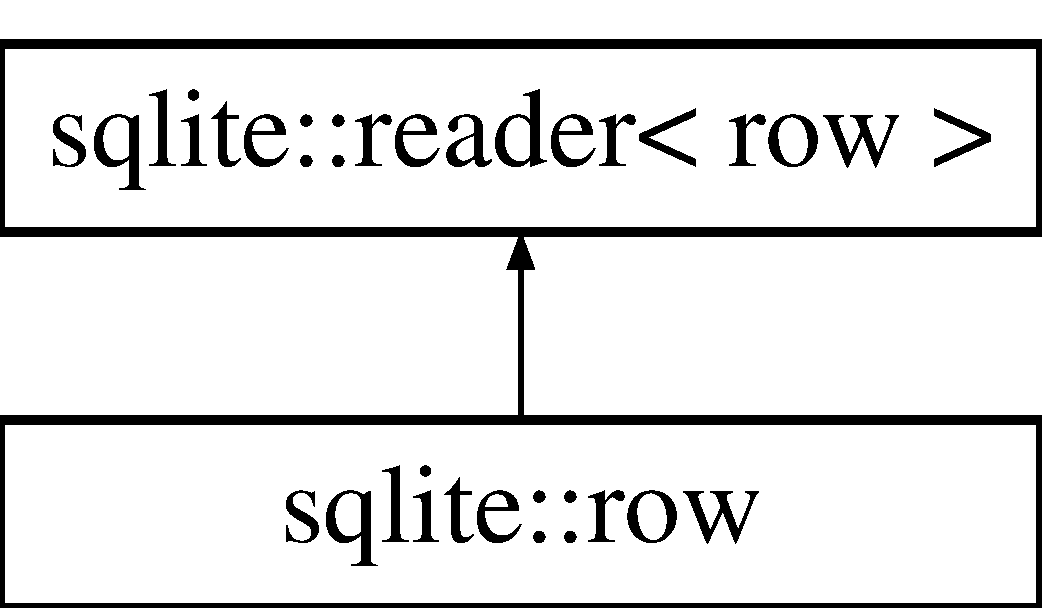
\includegraphics[height=2.000000cm]{a00011}
\end{center}
\end{figure}
\subsection*{Public Member Functions}
\begin{DoxyCompactItemize}
\item 
\hypertarget{a00011_ade44769ac78d6eff1aa20c20a09e4a79}{\hyperlink{a00011_ade44769ac78d6eff1aa20c20a09e4a79}{row} (sqlite3\-\_\-stmt $\ast$const \hyperlink{a00013}{statement}) noexcept}\label{a00011_ade44769ac78d6eff1aa20c20a09e4a79}

\begin{DoxyCompactList}\small\item\em Constructs a row object from a sqlite3\-\_\-stmt. \end{DoxyCompactList}\item 
\hypertarget{a00011_a6ee9eb13492a23d440abe1fe903bafc8}{sqlite3\-\_\-stmt $\ast$ \hyperlink{a00011_a6ee9eb13492a23d440abe1fe903bafc8}{handle} () const noexcept}\label{a00011_a6ee9eb13492a23d440abe1fe903bafc8}

\begin{DoxyCompactList}\small\item\em Returns pointer to the underlying \char`\"{}sqlite3\-\_\-stmt\char`\"{} object. \end{DoxyCompactList}\item 
\hyperlink{a00015}{value} \hyperlink{a00011_a0c8e886d5beb078d5111bdf812232c60}{operator\mbox{[}$\,$\mbox{]}} (int column) const 
\begin{DoxyCompactList}\small\item\em Access specified element of a row. \end{DoxyCompactList}\item 
\hyperlink{a00015}{value} \hyperlink{a00011_adcc08612b2968a75124edc91c0d6c72f}{operator\mbox{[}$\,$\mbox{]}} (const std\-::string \&name) const 
\begin{DoxyCompactList}\small\item\em Access specified element of a row. \end{DoxyCompactList}\item 
int \hyperlink{a00010_a1c720c80fd5c1f0f618c24a3d09e2ef5}{get\-\_\-int} (const int column) const noexcept
\begin{DoxyCompactList}\small\item\em Returns the specified column value as an integer. \end{DoxyCompactList}\item 
int \hyperlink{a00010_a7e1f86fdffd271cb92deb0b21d22fd05}{get\-\_\-int} (const std\-::string \&name) const noexcept
\begin{DoxyCompactList}\small\item\em Returns the specified column value as an integer. \end{DoxyCompactList}\item 
int64\-\_\-t \hyperlink{a00010_afaf16f586744a6bc0ecfb74ab791306c}{get\-\_\-int64} (const int column) const noexcept
\begin{DoxyCompactList}\small\item\em Returns the specified column value as a 64-\/bit integer. \end{DoxyCompactList}\item 
int64\-\_\-t \hyperlink{a00010_a87383f607d2ffc2875eac57ecf8e3989}{get\-\_\-int64} (const std\-::string \&name) const noexcept
\begin{DoxyCompactList}\small\item\em Returns the specified column value as a 64-\/bit integer. \end{DoxyCompactList}\item 
unsigned int \hyperlink{a00010_a02e09a2778e2f4d146ef02cd6c9e86df}{get\-\_\-uint} (const int column) const noexcept
\begin{DoxyCompactList}\small\item\em Returns the specified column value as an unsigned integer. \end{DoxyCompactList}\item 
unsigned int \hyperlink{a00010_a662bad64308f5995cb03a0ccb772acdc}{get\-\_\-uint} (const std\-::string \&name) const noexcept
\begin{DoxyCompactList}\small\item\em Returns the specified column value as an unsigned integer. \end{DoxyCompactList}\item 
double \hyperlink{a00010_aa4052f3e593580c81ba2b8622e2652eb}{get\-\_\-double} (const int column) const noexcept
\begin{DoxyCompactList}\small\item\em Returns the specified column value as a double. \end{DoxyCompactList}\item 
double \hyperlink{a00010_a0613aae6ee73cd54d7f7d0d711494737}{get\-\_\-double} (const std\-::string \&name) const noexcept
\begin{DoxyCompactList}\small\item\em Returns the specified column value as a double. \end{DoxyCompactList}\item 
const \hyperlink{a00002}{blob} \hyperlink{a00010_abd1b75c884158222778d2d6ec8b9ec18}{get\-\_\-blob} (const int column) const noexcept
\begin{DoxyCompactList}\small\item\em Returns the specified column value as a blob object. \end{DoxyCompactList}\item 
const \hyperlink{a00002}{blob} \hyperlink{a00010_a3a94b5c5a0d153ca7e2f0ef6719dfc9a}{get\-\_\-blob} (const std\-::string \&name) const noexcept
\begin{DoxyCompactList}\small\item\em Returns the specified column value as a Blob object. \end{DoxyCompactList}\item 
const std\-::string \hyperlink{a00010_a8716fe92a821ebc0799097bd6cc6d53c}{get\-\_\-string} (const int column) const noexcept
\begin{DoxyCompactList}\small\item\em Returns the specified column value as a string. \end{DoxyCompactList}\item 
const std\-::string \hyperlink{a00010_ab9c842deb81d9eb20388746672a96d29}{get\-\_\-string} (const std\-::string \&name) const noexcept
\begin{DoxyCompactList}\small\item\em Returns the specified column value as a string. \end{DoxyCompactList}\item 
const std\-::u16string \hyperlink{a00010_abfef02b657c992a2d07e28a07e41e533}{get\-\_\-u16string} (const int column) const noexcept
\begin{DoxyCompactList}\small\item\em Returns the specified column value as a U\-T\-F-\/16 string. \end{DoxyCompactList}\item 
const std\-::u16string \hyperlink{a00010_af10d3ff33e5f4ee471bc14cc41ec86c1}{get\-\_\-u16string} (const std\-::string \&name) const noexcept
\begin{DoxyCompactList}\small\item\em Returns the specified column value as a U\-T\-F-\/16 string. \end{DoxyCompactList}\item 
\hyperlink{a00015}{value} \hyperlink{a00010_af776fbdf8dc1150b628b04eca10841f4}{get\-\_\-value} (const int column) const noexcept
\begin{DoxyCompactList}\small\item\em Returns the specified column value as a value object. \end{DoxyCompactList}\item 
\hyperlink{a00015}{value} \hyperlink{a00010_ad7835e8a981450975fee7771fa863ffe}{get\-\_\-value} (const std\-::string \&name) const
\begin{DoxyCompactList}\small\item\em Returns the specified column value as a value object. \end{DoxyCompactList}\item 
int \hyperlink{a00010_ac4404227950aca8d5f01255a5541dbb4}{get\-\_\-bytes} (const int column) const noexcept
\begin{DoxyCompactList}\small\item\em Returns the size in bytes of the column value. \end{DoxyCompactList}\item 
int \hyperlink{a00010_a315b97406b5ba48bcd14857192d88d5e}{get\-\_\-bytes} (const std\-::string \&name) const noexcept
\begin{DoxyCompactList}\small\item\em Returns the size in bytes of the column value. \end{DoxyCompactList}\item 
datatype \hyperlink{a00010_a2b8269e0f9387afa36ab90eb55899dc4}{get\-\_\-type} (const int column) const noexcept
\begin{DoxyCompactList}\small\item\em Returns the type of the specified column. \end{DoxyCompactList}\item 
datatype \hyperlink{a00010_ac5ab606cf12aa4d2c9a183998420df44}{get\-\_\-type} (const std\-::string \&name) const noexcept
\begin{DoxyCompactList}\small\item\em Returns the type of the specified column. \end{DoxyCompactList}\item 
int \hyperlink{a00010_a7390afddbb1edc788f0afc6ce41f4562}{column\-\_\-count} () const noexcept
\begin{DoxyCompactList}\small\item\em Returns the number of columns in the result set returned by the prepared statement. \end{DoxyCompactList}\item 
const char $\ast$ \hyperlink{a00010_ad4c33f9b700a47c08f54e7b65afd34f2}{get\-\_\-column\-\_\-name} (const int index) const noexcept
\begin{DoxyCompactList}\small\item\em Returns the name assigned to a particular column. \end{DoxyCompactList}\item 
const char16\-\_\-t $\ast$ \hyperlink{a00010_aa7f2f528b10da75672e55fbc36566f9c}{get\-\_\-column\-\_\-wide\-\_\-name} (const int index) const noexcept
\begin{DoxyCompactList}\small\item\em Returns the name assigned to a particular column. \end{DoxyCompactList}\item 
int \hyperlink{a00010_aaca43590a209c2c7a0f7420c8a6c47b3}{get\-\_\-column\-\_\-index} (const std\-::string \&name) const
\begin{DoxyCompactList}\small\item\em Returns the position of a column with the specified name. \end{DoxyCompactList}\end{DoxyCompactItemize}


\subsection{Detailed Description}
Represents a returned row when stepping through a \char`\"{}\-S\-E\-L\-E\-C\-T\char`\"{} statement. 

Definition at line 307 of file Statement.\-h.



\subsection{Member Function Documentation}
\hypertarget{a00010_a7390afddbb1edc788f0afc6ce41f4562}{\index{sqlite\-::row@{sqlite\-::row}!column\-\_\-count@{column\-\_\-count}}
\index{column\-\_\-count@{column\-\_\-count}!sqlite::row@{sqlite\-::row}}
\subsubsection[{column\-\_\-count}]{\setlength{\rightskip}{0pt plus 5cm}int {\bf sqlite\-::reader}$<$ {\bf row}  $>$\-::column\-\_\-count (
\begin{DoxyParamCaption}
{}
\end{DoxyParamCaption}
) const\hspace{0.3cm}{\ttfamily [inline]}, {\ttfamily [noexcept]}, {\ttfamily [inherited]}}}\label{a00010_a7390afddbb1edc788f0afc6ce41f4562}


Returns the number of columns in the result set returned by the prepared statement. 

If this method returns 0, that means the prepared statment returns no data (for example an U\-P\-D\-A\-T\-E). \begin{DoxyReturn}{Returns}
The number of columns in the result set. 
\end{DoxyReturn}


Definition at line 234 of file Statement.\-h.

\hypertarget{a00010_abd1b75c884158222778d2d6ec8b9ec18}{\index{sqlite\-::row@{sqlite\-::row}!get\-\_\-blob@{get\-\_\-blob}}
\index{get\-\_\-blob@{get\-\_\-blob}!sqlite::row@{sqlite\-::row}}
\subsubsection[{get\-\_\-blob}]{\setlength{\rightskip}{0pt plus 5cm}const {\bf blob} {\bf sqlite\-::reader}$<$ {\bf row}  $>$\-::get\-\_\-blob (
\begin{DoxyParamCaption}
\item[{const int}]{column}
\end{DoxyParamCaption}
) const\hspace{0.3cm}{\ttfamily [inline]}, {\ttfamily [noexcept]}, {\ttfamily [inherited]}}}\label{a00010_abd1b75c884158222778d2d6ec8b9ec18}


Returns the specified column value as a blob object. 


\begin{DoxyParams}[1]{Parameters}
\mbox{\tt in}  & {\em column} & position of the column to return \\
\hline
\end{DoxyParams}
\begin{DoxyReturn}{Returns}
value of column as integer 
\end{DoxyReturn}


Definition at line 116 of file Statement.\-h.

\hypertarget{a00010_a3a94b5c5a0d153ca7e2f0ef6719dfc9a}{\index{sqlite\-::row@{sqlite\-::row}!get\-\_\-blob@{get\-\_\-blob}}
\index{get\-\_\-blob@{get\-\_\-blob}!sqlite::row@{sqlite\-::row}}
\subsubsection[{get\-\_\-blob}]{\setlength{\rightskip}{0pt plus 5cm}const {\bf blob} {\bf sqlite\-::reader}$<$ {\bf row}  $>$\-::get\-\_\-blob (
\begin{DoxyParamCaption}
\item[{const std\-::string \&}]{name}
\end{DoxyParamCaption}
) const\hspace{0.3cm}{\ttfamily [inline]}, {\ttfamily [noexcept]}, {\ttfamily [inherited]}}}\label{a00010_a3a94b5c5a0d153ca7e2f0ef6719dfc9a}


Returns the specified column value as a Blob object. 


\begin{DoxyParams}[1]{Parameters}
\mbox{\tt in}  & {\em name} & name of the column to return \\
\hline
\end{DoxyParams}
\begin{DoxyReturn}{Returns}
value of column as integer 
\end{DoxyReturn}


Definition at line 126 of file Statement.\-h.

\hypertarget{a00010_ac4404227950aca8d5f01255a5541dbb4}{\index{sqlite\-::row@{sqlite\-::row}!get\-\_\-bytes@{get\-\_\-bytes}}
\index{get\-\_\-bytes@{get\-\_\-bytes}!sqlite::row@{sqlite\-::row}}
\subsubsection[{get\-\_\-bytes}]{\setlength{\rightskip}{0pt plus 5cm}int {\bf sqlite\-::reader}$<$ {\bf row}  $>$\-::get\-\_\-bytes (
\begin{DoxyParamCaption}
\item[{const int}]{column}
\end{DoxyParamCaption}
) const\hspace{0.3cm}{\ttfamily [inline]}, {\ttfamily [noexcept]}, {\ttfamily [inherited]}}}\label{a00010_ac4404227950aca8d5f01255a5541dbb4}


Returns the size in bytes of the column value. 


\begin{DoxyParams}[1]{Parameters}
\mbox{\tt in}  & {\em column} & position of the column to return \\
\hline
\end{DoxyParams}
\begin{DoxyReturn}{Returns}
the size in bytes of the column value 
\end{DoxyReturn}


Definition at line 196 of file Statement.\-h.

\hypertarget{a00010_a315b97406b5ba48bcd14857192d88d5e}{\index{sqlite\-::row@{sqlite\-::row}!get\-\_\-bytes@{get\-\_\-bytes}}
\index{get\-\_\-bytes@{get\-\_\-bytes}!sqlite::row@{sqlite\-::row}}
\subsubsection[{get\-\_\-bytes}]{\setlength{\rightskip}{0pt plus 5cm}int {\bf sqlite\-::reader}$<$ {\bf row}  $>$\-::get\-\_\-bytes (
\begin{DoxyParamCaption}
\item[{const std\-::string \&}]{name}
\end{DoxyParamCaption}
) const\hspace{0.3cm}{\ttfamily [inline]}, {\ttfamily [noexcept]}, {\ttfamily [inherited]}}}\label{a00010_a315b97406b5ba48bcd14857192d88d5e}


Returns the size in bytes of the column value. 


\begin{DoxyParams}[1]{Parameters}
\mbox{\tt in}  & {\em name} & name of the column to return \\
\hline
\end{DoxyParams}
\begin{DoxyReturn}{Returns}
the size in bytes of the column value 
\end{DoxyReturn}


Definition at line 205 of file Statement.\-h.

\hypertarget{a00010_aaca43590a209c2c7a0f7420c8a6c47b3}{\index{sqlite\-::row@{sqlite\-::row}!get\-\_\-column\-\_\-index@{get\-\_\-column\-\_\-index}}
\index{get\-\_\-column\-\_\-index@{get\-\_\-column\-\_\-index}!sqlite::row@{sqlite\-::row}}
\subsubsection[{get\-\_\-column\-\_\-index}]{\setlength{\rightskip}{0pt plus 5cm}int {\bf sqlite\-::reader}$<$ {\bf row}  $>$\-::get\-\_\-column\-\_\-index (
\begin{DoxyParamCaption}
\item[{const std\-::string \&}]{name}
\end{DoxyParamCaption}
) const\hspace{0.3cm}{\ttfamily [inline]}, {\ttfamily [inherited]}}}\label{a00010_aaca43590a209c2c7a0f7420c8a6c47b3}


Returns the position of a column with the specified name. 

\begin{DoxyReturn}{Returns}
The position of the column 
\end{DoxyReturn}

\begin{DoxyExceptions}{Exceptions}
{\em S\-Q\-Lite\-X\-X\-Exception} & if no column with specified name was found \\
\hline
\end{DoxyExceptions}


Definition at line 261 of file Statement.\-h.

\hypertarget{a00010_ad4c33f9b700a47c08f54e7b65afd34f2}{\index{sqlite\-::row@{sqlite\-::row}!get\-\_\-column\-\_\-name@{get\-\_\-column\-\_\-name}}
\index{get\-\_\-column\-\_\-name@{get\-\_\-column\-\_\-name}!sqlite::row@{sqlite\-::row}}
\subsubsection[{get\-\_\-column\-\_\-name}]{\setlength{\rightskip}{0pt plus 5cm}const char$\ast$ {\bf sqlite\-::reader}$<$ {\bf row}  $>$\-::get\-\_\-column\-\_\-name (
\begin{DoxyParamCaption}
\item[{const int}]{index}
\end{DoxyParamCaption}
) const\hspace{0.3cm}{\ttfamily [inline]}, {\ttfamily [noexcept]}, {\ttfamily [inherited]}}}\label{a00010_ad4c33f9b700a47c08f54e7b65afd34f2}


Returns the name assigned to a particular column. 


\begin{DoxyParams}[1]{Parameters}
\mbox{\tt in}  & {\em index} & the position of the column \\
\hline
\end{DoxyParams}
\begin{DoxyReturn}{Returns}
The name of the specified column. 
\end{DoxyReturn}


Definition at line 243 of file Statement.\-h.

\hypertarget{a00010_aa7f2f528b10da75672e55fbc36566f9c}{\index{sqlite\-::row@{sqlite\-::row}!get\-\_\-column\-\_\-wide\-\_\-name@{get\-\_\-column\-\_\-wide\-\_\-name}}
\index{get\-\_\-column\-\_\-wide\-\_\-name@{get\-\_\-column\-\_\-wide\-\_\-name}!sqlite::row@{sqlite\-::row}}
\subsubsection[{get\-\_\-column\-\_\-wide\-\_\-name}]{\setlength{\rightskip}{0pt plus 5cm}const char16\-\_\-t$\ast$ {\bf sqlite\-::reader}$<$ {\bf row}  $>$\-::get\-\_\-column\-\_\-wide\-\_\-name (
\begin{DoxyParamCaption}
\item[{const int}]{index}
\end{DoxyParamCaption}
) const\hspace{0.3cm}{\ttfamily [inline]}, {\ttfamily [noexcept]}, {\ttfamily [inherited]}}}\label{a00010_aa7f2f528b10da75672e55fbc36566f9c}


Returns the name assigned to a particular column. 


\begin{DoxyParams}[1]{Parameters}
\mbox{\tt in}  & {\em index} & the position of the column \\
\hline
\end{DoxyParams}
\begin{DoxyReturn}{Returns}
The name of the specified column. 
\end{DoxyReturn}


Definition at line 252 of file Statement.\-h.

\hypertarget{a00010_aa4052f3e593580c81ba2b8622e2652eb}{\index{sqlite\-::row@{sqlite\-::row}!get\-\_\-double@{get\-\_\-double}}
\index{get\-\_\-double@{get\-\_\-double}!sqlite::row@{sqlite\-::row}}
\subsubsection[{get\-\_\-double}]{\setlength{\rightskip}{0pt plus 5cm}double {\bf sqlite\-::reader}$<$ {\bf row}  $>$\-::get\-\_\-double (
\begin{DoxyParamCaption}
\item[{const int}]{column}
\end{DoxyParamCaption}
) const\hspace{0.3cm}{\ttfamily [inline]}, {\ttfamily [noexcept]}, {\ttfamily [inherited]}}}\label{a00010_aa4052f3e593580c81ba2b8622e2652eb}


Returns the specified column value as a double. 


\begin{DoxyParams}[1]{Parameters}
\mbox{\tt in}  & {\em column} & position of the column to return \\
\hline
\end{DoxyParams}
\begin{DoxyReturn}{Returns}
value of column as integer 
\end{DoxyReturn}


Definition at line 97 of file Statement.\-h.

\hypertarget{a00010_a0613aae6ee73cd54d7f7d0d711494737}{\index{sqlite\-::row@{sqlite\-::row}!get\-\_\-double@{get\-\_\-double}}
\index{get\-\_\-double@{get\-\_\-double}!sqlite::row@{sqlite\-::row}}
\subsubsection[{get\-\_\-double}]{\setlength{\rightskip}{0pt plus 5cm}double {\bf sqlite\-::reader}$<$ {\bf row}  $>$\-::get\-\_\-double (
\begin{DoxyParamCaption}
\item[{const std\-::string \&}]{name}
\end{DoxyParamCaption}
) const\hspace{0.3cm}{\ttfamily [inline]}, {\ttfamily [noexcept]}, {\ttfamily [inherited]}}}\label{a00010_a0613aae6ee73cd54d7f7d0d711494737}


Returns the specified column value as a double. 


\begin{DoxyParams}[1]{Parameters}
\mbox{\tt in}  & {\em name} & name of the column to return \\
\hline
\end{DoxyParams}
\begin{DoxyReturn}{Returns}
value of column as integer 
\end{DoxyReturn}


Definition at line 106 of file Statement.\-h.

\hypertarget{a00010_a1c720c80fd5c1f0f618c24a3d09e2ef5}{\index{sqlite\-::row@{sqlite\-::row}!get\-\_\-int@{get\-\_\-int}}
\index{get\-\_\-int@{get\-\_\-int}!sqlite::row@{sqlite\-::row}}
\subsubsection[{get\-\_\-int}]{\setlength{\rightskip}{0pt plus 5cm}int {\bf sqlite\-::reader}$<$ {\bf row}  $>$\-::get\-\_\-int (
\begin{DoxyParamCaption}
\item[{const int}]{column}
\end{DoxyParamCaption}
) const\hspace{0.3cm}{\ttfamily [inline]}, {\ttfamily [noexcept]}, {\ttfamily [inherited]}}}\label{a00010_a1c720c80fd5c1f0f618c24a3d09e2ef5}


Returns the specified column value as an integer. 


\begin{DoxyParams}[1]{Parameters}
\mbox{\tt in}  & {\em column} & position of the column to return \\
\hline
\end{DoxyParams}
\begin{DoxyReturn}{Returns}
value of column as integer 
\end{DoxyReturn}


Definition at line 40 of file Statement.\-h.

\hypertarget{a00010_a7e1f86fdffd271cb92deb0b21d22fd05}{\index{sqlite\-::row@{sqlite\-::row}!get\-\_\-int@{get\-\_\-int}}
\index{get\-\_\-int@{get\-\_\-int}!sqlite::row@{sqlite\-::row}}
\subsubsection[{get\-\_\-int}]{\setlength{\rightskip}{0pt plus 5cm}int {\bf sqlite\-::reader}$<$ {\bf row}  $>$\-::get\-\_\-int (
\begin{DoxyParamCaption}
\item[{const std\-::string \&}]{name}
\end{DoxyParamCaption}
) const\hspace{0.3cm}{\ttfamily [inline]}, {\ttfamily [noexcept]}, {\ttfamily [inherited]}}}\label{a00010_a7e1f86fdffd271cb92deb0b21d22fd05}


Returns the specified column value as an integer. 


\begin{DoxyParams}[1]{Parameters}
\mbox{\tt in}  & {\em name} & name of the column to return \\
\hline
\end{DoxyParams}
\begin{DoxyReturn}{Returns}
value of column as integer 
\end{DoxyReturn}


Definition at line 49 of file Statement.\-h.

\hypertarget{a00010_afaf16f586744a6bc0ecfb74ab791306c}{\index{sqlite\-::row@{sqlite\-::row}!get\-\_\-int64@{get\-\_\-int64}}
\index{get\-\_\-int64@{get\-\_\-int64}!sqlite::row@{sqlite\-::row}}
\subsubsection[{get\-\_\-int64}]{\setlength{\rightskip}{0pt plus 5cm}int64\-\_\-t {\bf sqlite\-::reader}$<$ {\bf row}  $>$\-::get\-\_\-int64 (
\begin{DoxyParamCaption}
\item[{const int}]{column}
\end{DoxyParamCaption}
) const\hspace{0.3cm}{\ttfamily [inline]}, {\ttfamily [noexcept]}, {\ttfamily [inherited]}}}\label{a00010_afaf16f586744a6bc0ecfb74ab791306c}


Returns the specified column value as a 64-\/bit integer. 


\begin{DoxyParams}[1]{Parameters}
\mbox{\tt in}  & {\em column} & position of the column to return \\
\hline
\end{DoxyParams}
\begin{DoxyReturn}{Returns}
value of column as integer 
\end{DoxyReturn}


Definition at line 59 of file Statement.\-h.

\hypertarget{a00010_a87383f607d2ffc2875eac57ecf8e3989}{\index{sqlite\-::row@{sqlite\-::row}!get\-\_\-int64@{get\-\_\-int64}}
\index{get\-\_\-int64@{get\-\_\-int64}!sqlite::row@{sqlite\-::row}}
\subsubsection[{get\-\_\-int64}]{\setlength{\rightskip}{0pt plus 5cm}int64\-\_\-t {\bf sqlite\-::reader}$<$ {\bf row}  $>$\-::get\-\_\-int64 (
\begin{DoxyParamCaption}
\item[{const std\-::string \&}]{name}
\end{DoxyParamCaption}
) const\hspace{0.3cm}{\ttfamily [inline]}, {\ttfamily [noexcept]}, {\ttfamily [inherited]}}}\label{a00010_a87383f607d2ffc2875eac57ecf8e3989}


Returns the specified column value as a 64-\/bit integer. 


\begin{DoxyParams}[1]{Parameters}
\mbox{\tt in}  & {\em name} & name of the column to return \\
\hline
\end{DoxyParams}
\begin{DoxyReturn}{Returns}
value of column as integer 
\end{DoxyReturn}


Definition at line 68 of file Statement.\-h.

\hypertarget{a00010_a8716fe92a821ebc0799097bd6cc6d53c}{\index{sqlite\-::row@{sqlite\-::row}!get\-\_\-string@{get\-\_\-string}}
\index{get\-\_\-string@{get\-\_\-string}!sqlite::row@{sqlite\-::row}}
\subsubsection[{get\-\_\-string}]{\setlength{\rightskip}{0pt plus 5cm}const std\-::string {\bf sqlite\-::reader}$<$ {\bf row}  $>$\-::get\-\_\-string (
\begin{DoxyParamCaption}
\item[{const int}]{column}
\end{DoxyParamCaption}
) const\hspace{0.3cm}{\ttfamily [inline]}, {\ttfamily [noexcept]}, {\ttfamily [inherited]}}}\label{a00010_a8716fe92a821ebc0799097bd6cc6d53c}


Returns the specified column value as a string. 


\begin{DoxyParams}[1]{Parameters}
\mbox{\tt in}  & {\em column} & position of the column to return \\
\hline
\end{DoxyParams}
\begin{DoxyReturn}{Returns}
value of column as integer 
\end{DoxyReturn}


Definition at line 136 of file Statement.\-h.

\hypertarget{a00010_ab9c842deb81d9eb20388746672a96d29}{\index{sqlite\-::row@{sqlite\-::row}!get\-\_\-string@{get\-\_\-string}}
\index{get\-\_\-string@{get\-\_\-string}!sqlite::row@{sqlite\-::row}}
\subsubsection[{get\-\_\-string}]{\setlength{\rightskip}{0pt plus 5cm}const std\-::string {\bf sqlite\-::reader}$<$ {\bf row}  $>$\-::get\-\_\-string (
\begin{DoxyParamCaption}
\item[{const std\-::string \&}]{name}
\end{DoxyParamCaption}
) const\hspace{0.3cm}{\ttfamily [inline]}, {\ttfamily [noexcept]}, {\ttfamily [inherited]}}}\label{a00010_ab9c842deb81d9eb20388746672a96d29}


Returns the specified column value as a string. 


\begin{DoxyParams}[1]{Parameters}
\mbox{\tt in}  & {\em name} & name of the column to return \\
\hline
\end{DoxyParams}
\begin{DoxyReturn}{Returns}
value of column as integer 
\end{DoxyReturn}


Definition at line 146 of file Statement.\-h.

\hypertarget{a00010_a2b8269e0f9387afa36ab90eb55899dc4}{\index{sqlite\-::row@{sqlite\-::row}!get\-\_\-type@{get\-\_\-type}}
\index{get\-\_\-type@{get\-\_\-type}!sqlite::row@{sqlite\-::row}}
\subsubsection[{get\-\_\-type}]{\setlength{\rightskip}{0pt plus 5cm}datatype {\bf sqlite\-::reader}$<$ {\bf row}  $>$\-::get\-\_\-type (
\begin{DoxyParamCaption}
\item[{const int}]{column}
\end{DoxyParamCaption}
) const\hspace{0.3cm}{\ttfamily [inline]}, {\ttfamily [noexcept]}, {\ttfamily [inherited]}}}\label{a00010_a2b8269e0f9387afa36ab90eb55899dc4}


Returns the type of the specified column. 


\begin{DoxyParams}[1]{Parameters}
\mbox{\tt in}  & {\em column} & position of the column to return \\
\hline
\end{DoxyParams}
\begin{DoxyReturn}{Returns}
The sqlite\-::datatype value for a column 
\end{DoxyReturn}


Definition at line 215 of file Statement.\-h.

\hypertarget{a00010_ac5ab606cf12aa4d2c9a183998420df44}{\index{sqlite\-::row@{sqlite\-::row}!get\-\_\-type@{get\-\_\-type}}
\index{get\-\_\-type@{get\-\_\-type}!sqlite::row@{sqlite\-::row}}
\subsubsection[{get\-\_\-type}]{\setlength{\rightskip}{0pt plus 5cm}datatype {\bf sqlite\-::reader}$<$ {\bf row}  $>$\-::get\-\_\-type (
\begin{DoxyParamCaption}
\item[{const std\-::string \&}]{name}
\end{DoxyParamCaption}
) const\hspace{0.3cm}{\ttfamily [inline]}, {\ttfamily [noexcept]}, {\ttfamily [inherited]}}}\label{a00010_ac5ab606cf12aa4d2c9a183998420df44}


Returns the type of the specified column. 


\begin{DoxyParams}[1]{Parameters}
\mbox{\tt in}  & {\em name} & name of the column to return \\
\hline
\end{DoxyParams}
\begin{DoxyReturn}{Returns}
The sqlite\-::datatype value for a column 
\end{DoxyReturn}


Definition at line 224 of file Statement.\-h.

\hypertarget{a00010_abfef02b657c992a2d07e28a07e41e533}{\index{sqlite\-::row@{sqlite\-::row}!get\-\_\-u16string@{get\-\_\-u16string}}
\index{get\-\_\-u16string@{get\-\_\-u16string}!sqlite::row@{sqlite\-::row}}
\subsubsection[{get\-\_\-u16string}]{\setlength{\rightskip}{0pt plus 5cm}const std\-::u16string {\bf sqlite\-::reader}$<$ {\bf row}  $>$\-::get\-\_\-u16string (
\begin{DoxyParamCaption}
\item[{const int}]{column}
\end{DoxyParamCaption}
) const\hspace{0.3cm}{\ttfamily [inline]}, {\ttfamily [noexcept]}, {\ttfamily [inherited]}}}\label{a00010_abfef02b657c992a2d07e28a07e41e533}


Returns the specified column value as a U\-T\-F-\/16 string. 


\begin{DoxyParams}[1]{Parameters}
\mbox{\tt in}  & {\em column} & position of the column to return \\
\hline
\end{DoxyParams}
\begin{DoxyReturn}{Returns}
value of column as integer 
\end{DoxyReturn}


Definition at line 156 of file Statement.\-h.

\hypertarget{a00010_af10d3ff33e5f4ee471bc14cc41ec86c1}{\index{sqlite\-::row@{sqlite\-::row}!get\-\_\-u16string@{get\-\_\-u16string}}
\index{get\-\_\-u16string@{get\-\_\-u16string}!sqlite::row@{sqlite\-::row}}
\subsubsection[{get\-\_\-u16string}]{\setlength{\rightskip}{0pt plus 5cm}const std\-::u16string {\bf sqlite\-::reader}$<$ {\bf row}  $>$\-::get\-\_\-u16string (
\begin{DoxyParamCaption}
\item[{const std\-::string \&}]{name}
\end{DoxyParamCaption}
) const\hspace{0.3cm}{\ttfamily [inline]}, {\ttfamily [noexcept]}, {\ttfamily [inherited]}}}\label{a00010_af10d3ff33e5f4ee471bc14cc41ec86c1}


Returns the specified column value as a U\-T\-F-\/16 string. 


\begin{DoxyParams}[1]{Parameters}
\mbox{\tt in}  & {\em name} & name of the column to return \\
\hline
\end{DoxyParams}
\begin{DoxyReturn}{Returns}
value of column as integer 
\end{DoxyReturn}


Definition at line 166 of file Statement.\-h.

\hypertarget{a00010_a02e09a2778e2f4d146ef02cd6c9e86df}{\index{sqlite\-::row@{sqlite\-::row}!get\-\_\-uint@{get\-\_\-uint}}
\index{get\-\_\-uint@{get\-\_\-uint}!sqlite::row@{sqlite\-::row}}
\subsubsection[{get\-\_\-uint}]{\setlength{\rightskip}{0pt plus 5cm}unsigned int {\bf sqlite\-::reader}$<$ {\bf row}  $>$\-::get\-\_\-uint (
\begin{DoxyParamCaption}
\item[{const int}]{column}
\end{DoxyParamCaption}
) const\hspace{0.3cm}{\ttfamily [inline]}, {\ttfamily [noexcept]}, {\ttfamily [inherited]}}}\label{a00010_a02e09a2778e2f4d146ef02cd6c9e86df}


Returns the specified column value as an unsigned integer. 


\begin{DoxyParams}[1]{Parameters}
\mbox{\tt in}  & {\em column} & position of the column to return \\
\hline
\end{DoxyParams}
\begin{DoxyReturn}{Returns}
value of column as integer 
\end{DoxyReturn}


Definition at line 78 of file Statement.\-h.

\hypertarget{a00010_a662bad64308f5995cb03a0ccb772acdc}{\index{sqlite\-::row@{sqlite\-::row}!get\-\_\-uint@{get\-\_\-uint}}
\index{get\-\_\-uint@{get\-\_\-uint}!sqlite::row@{sqlite\-::row}}
\subsubsection[{get\-\_\-uint}]{\setlength{\rightskip}{0pt plus 5cm}unsigned int {\bf sqlite\-::reader}$<$ {\bf row}  $>$\-::get\-\_\-uint (
\begin{DoxyParamCaption}
\item[{const std\-::string \&}]{name}
\end{DoxyParamCaption}
) const\hspace{0.3cm}{\ttfamily [inline]}, {\ttfamily [noexcept]}, {\ttfamily [inherited]}}}\label{a00010_a662bad64308f5995cb03a0ccb772acdc}


Returns the specified column value as an unsigned integer. 


\begin{DoxyParams}[1]{Parameters}
\mbox{\tt in}  & {\em name} & name of the column to return \\
\hline
\end{DoxyParams}
\begin{DoxyReturn}{Returns}
value of column as integer 
\end{DoxyReturn}


Definition at line 87 of file Statement.\-h.

\hypertarget{a00010_af776fbdf8dc1150b628b04eca10841f4}{\index{sqlite\-::row@{sqlite\-::row}!get\-\_\-value@{get\-\_\-value}}
\index{get\-\_\-value@{get\-\_\-value}!sqlite::row@{sqlite\-::row}}
\subsubsection[{get\-\_\-value}]{\setlength{\rightskip}{0pt plus 5cm}{\bf value} {\bf sqlite\-::reader}$<$ {\bf row}  $>$\-::get\-\_\-value (
\begin{DoxyParamCaption}
\item[{const int}]{column}
\end{DoxyParamCaption}
) const\hspace{0.3cm}{\ttfamily [inline]}, {\ttfamily [noexcept]}, {\ttfamily [inherited]}}}\label{a00010_af776fbdf8dc1150b628b04eca10841f4}


Returns the specified column value as a value object. 


\begin{DoxyParams}[1]{Parameters}
\mbox{\tt in}  & {\em column} & position of the column to return \\
\hline
\end{DoxyParams}
\begin{DoxyReturn}{Returns}
value of column as integer 
\end{DoxyReturn}


Definition at line 176 of file Statement.\-h.

\hypertarget{a00010_ad7835e8a981450975fee7771fa863ffe}{\index{sqlite\-::row@{sqlite\-::row}!get\-\_\-value@{get\-\_\-value}}
\index{get\-\_\-value@{get\-\_\-value}!sqlite::row@{sqlite\-::row}}
\subsubsection[{get\-\_\-value}]{\setlength{\rightskip}{0pt plus 5cm}{\bf value} {\bf sqlite\-::reader}$<$ {\bf row}  $>$\-::get\-\_\-value (
\begin{DoxyParamCaption}
\item[{const std\-::string \&}]{name}
\end{DoxyParamCaption}
) const\hspace{0.3cm}{\ttfamily [inline]}, {\ttfamily [inherited]}}}\label{a00010_ad7835e8a981450975fee7771fa863ffe}


Returns the specified column value as a value object. 


\begin{DoxyParams}[1]{Parameters}
\mbox{\tt in}  & {\em name} & name of the column to return \\
\hline
\end{DoxyParams}
\begin{DoxyReturn}{Returns}
value of column as integer 
\end{DoxyReturn}


Definition at line 185 of file Statement.\-h.

\hypertarget{a00011_a0c8e886d5beb078d5111bdf812232c60}{\index{sqlite\-::row@{sqlite\-::row}!operator\mbox{[}$\,$\mbox{]}@{operator[]}}
\index{operator\mbox{[}$\,$\mbox{]}@{operator[]}!sqlite::row@{sqlite\-::row}}
\subsubsection[{operator[]}]{\setlength{\rightskip}{0pt plus 5cm}{\bf value} sqlite\-::row\-::operator\mbox{[}$\,$\mbox{]} (
\begin{DoxyParamCaption}
\item[{int}]{column}
\end{DoxyParamCaption}
) const\hspace{0.3cm}{\ttfamily [inline]}}}\label{a00011_a0c8e886d5beb078d5111bdf812232c60}


Access specified element of a row. 


\begin{DoxyParams}[1]{Parameters}
\mbox{\tt in}  & {\em column} & position of the column to return \\
\hline
\end{DoxyParams}
\begin{DoxyReturn}{Returns}
value object representing requested element 
\end{DoxyReturn}


Definition at line 328 of file Statement.\-h.

\hypertarget{a00011_adcc08612b2968a75124edc91c0d6c72f}{\index{sqlite\-::row@{sqlite\-::row}!operator\mbox{[}$\,$\mbox{]}@{operator[]}}
\index{operator\mbox{[}$\,$\mbox{]}@{operator[]}!sqlite::row@{sqlite\-::row}}
\subsubsection[{operator[]}]{\setlength{\rightskip}{0pt plus 5cm}{\bf value} sqlite\-::row\-::operator\mbox{[}$\,$\mbox{]} (
\begin{DoxyParamCaption}
\item[{const std\-::string \&}]{name}
\end{DoxyParamCaption}
) const\hspace{0.3cm}{\ttfamily [inline]}}}\label{a00011_adcc08612b2968a75124edc91c0d6c72f}


Access specified element of a row. 


\begin{DoxyParams}[1]{Parameters}
\mbox{\tt in}  & {\em name} & column name of the column to return \\
\hline
\end{DoxyParams}
\begin{DoxyReturn}{Returns}
value object representing requested element 
\end{DoxyReturn}


Definition at line 337 of file Statement.\-h.



The documentation for this class was generated from the following file\-:\begin{DoxyCompactItemize}
\item 
src/\hyperlink{a00032}{Statement.\-h}\end{DoxyCompactItemize}

\hypertarget{a00012}{\section{sqlite\-:\-:row\-\_\-iterator Class Reference}
\label{a00012}\index{sqlite\-::row\-\_\-iterator@{sqlite\-::row\-\_\-iterator}}
}


Helps when iterating over rows in a \char`\"{}\-S\-E\-L\-E\-C\-T\char`\"{} statement.  




{\ttfamily \#include $<$Statement.\-h$>$}

\subsection*{Public Member Functions}
\begin{DoxyCompactItemize}
\item 
\hypertarget{a00012_a02cfc59ac9cfeb41adbd7c28be6a6200}{\hyperlink{a00012_a02cfc59ac9cfeb41adbd7c28be6a6200}{row\-\_\-iterator} () noexcept=default}\label{a00012_a02cfc59ac9cfeb41adbd7c28be6a6200}

\begin{DoxyCompactList}\small\item\em Default constructor. \end{DoxyCompactList}\item 
\hyperlink{a00012_aa4ac6c92c4db3e59cea7984d8db3d587}{row\-\_\-iterator} (const \hyperlink{a00013}{statement} \&\hyperlink{a00013}{statement}) noexcept
\begin{DoxyCompactList}\small\item\em Construct a \hyperlink{a00012}{row\-\_\-iterator} object from a statement object. \end{DoxyCompactList}\item 
\hypertarget{a00012_a5485c5c0f9f04cbff43dfb285dc6e776}{\hyperlink{a00012}{row\-\_\-iterator} \& \hyperlink{a00012_a5485c5c0f9f04cbff43dfb285dc6e776}{operator++} () noexcept}\label{a00012_a5485c5c0f9f04cbff43dfb285dc6e776}

\begin{DoxyCompactList}\small\item\em Increment iterator to the next row object of the statement. \end{DoxyCompactList}\item 
\hypertarget{a00012_a618bc4f69040dcc2658719ab1a721be1}{bool \hyperlink{a00012_a618bc4f69040dcc2658719ab1a721be1}{operator!=} (const \hyperlink{a00012}{row\-\_\-iterator} \&other) const noexcept}\label{a00012_a618bc4f69040dcc2658719ab1a721be1}

\begin{DoxyCompactList}\small\item\em Comparison operation. \end{DoxyCompactList}\item 
\hyperlink{a00011}{row} \hyperlink{a00012_a5f2c042f06e9e03db0c24e9f1eee3e13}{operator$\ast$} () const noexcept
\begin{DoxyCompactList}\small\item\em Dereference operation. \end{DoxyCompactList}\end{DoxyCompactItemize}


\subsection{Detailed Description}
Helps when iterating over rows in a \char`\"{}\-S\-E\-L\-E\-C\-T\char`\"{} statement. 

\hyperlink{a00012}{row\-\_\-iterator} is a \href{http://en.cppreference.com/w/cpp/concept/InputIterator}{\tt Input\-Iterator} and can read data from the pointed to S\-Q\-Lite row. 

Definition at line 592 of file Statement.\-h.



\subsection{Constructor \& Destructor Documentation}
\hypertarget{a00012_aa4ac6c92c4db3e59cea7984d8db3d587}{\index{sqlite\-::row\-\_\-iterator@{sqlite\-::row\-\_\-iterator}!row\-\_\-iterator@{row\-\_\-iterator}}
\index{row\-\_\-iterator@{row\-\_\-iterator}!sqlite::row_iterator@{sqlite\-::row\-\_\-iterator}}
\subsubsection[{row\-\_\-iterator}]{\setlength{\rightskip}{0pt plus 5cm}sqlite\-::row\-\_\-iterator\-::row\-\_\-iterator (
\begin{DoxyParamCaption}
\item[{const {\bf statement} \&}]{statement}
\end{DoxyParamCaption}
)\hspace{0.3cm}{\ttfamily [noexcept]}}}\label{a00012_aa4ac6c92c4db3e59cea7984d8db3d587}


Construct a \hyperlink{a00012}{row\-\_\-iterator} object from a statement object. 

A \hyperlink{a00012}{row\-\_\-iterator} should only be constructect on an statement object that is doing a S\-Q\-L \char`\"{}\-S\-E\-L\-E\-C\-T\char`\"{} query. 
\begin{DoxyParams}{Parameters}
{\em statement} & the statement object to construct the iterator from. \\
\hline
\end{DoxyParams}


Definition at line 131 of file Statement.\-cpp.



\subsection{Member Function Documentation}
\hypertarget{a00012_a5f2c042f06e9e03db0c24e9f1eee3e13}{\index{sqlite\-::row\-\_\-iterator@{sqlite\-::row\-\_\-iterator}!operator$\ast$@{operator$\ast$}}
\index{operator$\ast$@{operator$\ast$}!sqlite::row_iterator@{sqlite\-::row\-\_\-iterator}}
\subsubsection[{operator$\ast$}]{\setlength{\rightskip}{0pt plus 5cm}{\bf row} sqlite\-::row\-\_\-iterator\-::operator$\ast$ (
\begin{DoxyParamCaption}
{}
\end{DoxyParamCaption}
) const\hspace{0.3cm}{\ttfamily [noexcept]}}}\label{a00012_a5f2c042f06e9e03db0c24e9f1eee3e13}


Dereference operation. 

Dereferencing a \hyperlink{a00012}{row\-\_\-iterator} object will return a row object. 

Definition at line 154 of file Statement.\-cpp.



The documentation for this class was generated from the following files\-:\begin{DoxyCompactItemize}
\item 
src/\hyperlink{a00032}{Statement.\-h}\item 
src/Statement.\-cpp\end{DoxyCompactItemize}

\hypertarget{a00013}{\section{S\-Q\-Lite\-:\-:Statement Class Reference}
\label{a00013}\index{S\-Q\-Lite\-::\-Statement@{S\-Q\-Lite\-::\-Statement}}
}


Represents a single S\-Q\-L statement that has been compiled into binary form and is ready to be evaluated, aka \char`\"{}sqlite3\-\_\-stmt\char`\"{}.  




{\ttfamily \#include $<$Statement.\-h$>$}

Inheritance diagram for S\-Q\-Lite\-:\-:Statement\-:\begin{figure}[H]
\begin{center}
\leavevmode
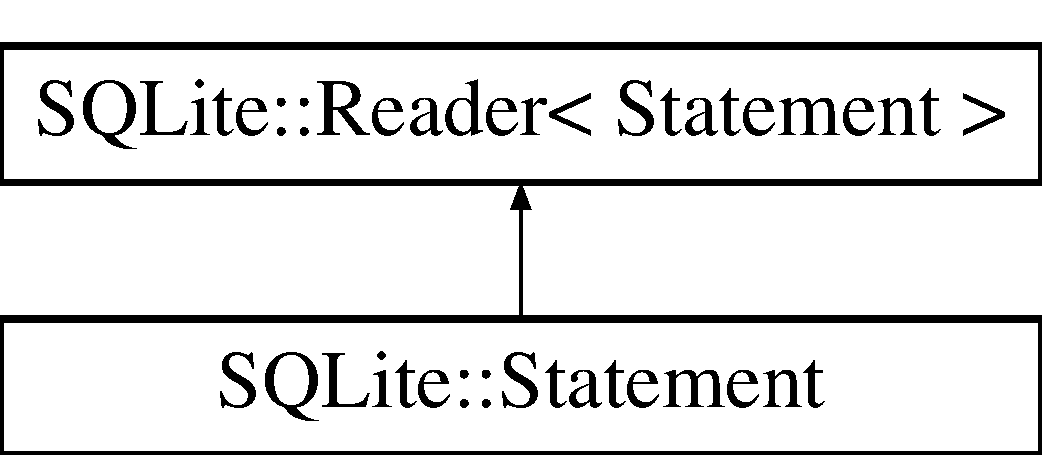
\includegraphics[height=2.000000cm]{a00013}
\end{center}
\end{figure}
\subsection*{Public Member Functions}
\begin{DoxyCompactItemize}
\item 
\hyperlink{a00013_a1c724c3934925a5988aa83909857589c}{Statement} () noexcept
\begin{DoxyCompactList}\small\item\em Default constructor. \end{DoxyCompactList}\item 
{\footnotesize template$<$typename... Values$>$ }\\\hyperlink{a00013_ac4f1af971f094f30c445bcc18ffc4e27}{Statement} (const \hyperlink{a00004}{D\-B\-Connection} \&connection, const std\-::string \&text, Values \&\&...values)
\begin{DoxyCompactList}\small\item\em Creates, prepares, and binds values into an S\-Q\-L statement. \end{DoxyCompactList}\item 
{\footnotesize template$<$typename... Values$>$ }\\\hyperlink{a00013_a3857ee340dd2769fafe10259cf4858a3}{Statement} (const \hyperlink{a00004}{D\-B\-Connection} \&connection, const std\-::u16string \&text, Values \&\&...values)
\begin{DoxyCompactList}\small\item\em Creates, prepares, and binds values into an S\-Q\-L statement. \end{DoxyCompactList}\item 
\hyperlink{a00013_a3b7793f1490a321159690cf096ec74d6}{operator bool} () const noexcept
\begin{DoxyCompactList}\small\item\em Used to specify if the \hyperlink{a00013}{Statement} object has a prepared \hyperlink{a00038}{S\-Q\-Lite} statement. \end{DoxyCompactList}\item 
sqlite3\-\_\-stmt $\ast$ \hyperlink{a00013_a9052c143879aca6cf253925336464a8b}{get\-Handle} () const noexcept
\begin{DoxyCompactList}\small\item\em Returns pointer to the underlying \char`\"{}sqlite3\-\_\-stmt\char`\"{} object. \end{DoxyCompactList}\item 
{\footnotesize template$<$typename... Values$>$ }\\void \hyperlink{a00013_a1ecd8e2636b542314521eb68fbf1000e}{prepare} (\hyperlink{a00004}{D\-B\-Connection} const \&connection, const std\-::string \&text, Values \&\&...values)
\begin{DoxyCompactList}\small\item\em Turn an S\-Q\-L query into byte code. \end{DoxyCompactList}\item 
{\footnotesize template$<$typename... Values$>$ }\\void \hyperlink{a00013_a0d422eadca4b2e3f2e1b6e13af69f3cc}{prepare} (const \hyperlink{a00004}{D\-B\-Connection} \&connection, const std\-::u16string \&text, Values \&\&...values)
\begin{DoxyCompactList}\small\item\em Turn an S\-Q\-L query into byte code. \end{DoxyCompactList}\item 
bool \hyperlink{a00013_a6251d1119e978d1366113b4aa30899ef}{step} () const 
\begin{DoxyCompactList}\small\item\em Evaluates a prepared statement. \end{DoxyCompactList}\item 
int \hyperlink{a00013_a9b489a2dc2707543eba55ce1e5d3682c}{execute} () const 
\begin{DoxyCompactList}\small\item\em Executes a prepared statement and will return the number of changes to the database. \end{DoxyCompactList}\item 
void \hyperlink{a00013_a0d4999fce90145852287c18c0d218ac6}{bind} (const int index, const int value) const 
\begin{DoxyCompactList}\small\item\em Binds an integer value to a parameter in an S\-Q\-L prepared statement. \end{DoxyCompactList}\item 
void \hyperlink{a00013_ace8156c735b1e630e82a3840910e02cf}{bind} (const int index, const double value) const 
\begin{DoxyCompactList}\small\item\em Binds an double value to a parameter in an S\-Q\-L prepared statement. \end{DoxyCompactList}\item 
void \hyperlink{a00013_aab00e4b2d9a0d85ccaf2b058d0cc9523}{bind} (const int index, const void $\ast$const value, const int size, \hyperlink{a00038_a32877e51b309dd8f2a28c21c0ba4a6fd}{Bind\-Type} type=\hyperlink{a00038_a32877e51b309dd8f2a28c21c0ba4a6fdab1f023eff9a6b5308d6024e4c6b3d475}{Bind\-Type\-::\-Transient}) const 
\begin{DoxyCompactList}\small\item\em Binds an blob value to a parameter in an S\-Q\-L prepared statement. \end{DoxyCompactList}\item 
void \hyperlink{a00013_afc5e0d9485bfedc71e9863cdb3c3d11a}{bind} (const int index, const \hyperlink{a00002}{Blob} \&value) const 
\begin{DoxyCompactList}\small\item\em Binds an \hyperlink{a00002}{Blob} value to a parameter in an S\-Q\-L prepared statement. \end{DoxyCompactList}\item 
void \hyperlink{a00013_a3ed628586d99205a1443790e7dc1e36f}{bind} (const int index, const char $\ast$const value, const int size=-\/1, \hyperlink{a00038_a32877e51b309dd8f2a28c21c0ba4a6fd}{Bind\-Type} type=\hyperlink{a00038_a32877e51b309dd8f2a28c21c0ba4a6fdab1f023eff9a6b5308d6024e4c6b3d475}{Bind\-Type\-::\-Transient}) const 
\begin{DoxyCompactList}\small\item\em Binds an string value to a parameter in an S\-Q\-L prepared statement. \end{DoxyCompactList}\item 
void \hyperlink{a00013_a6b983503e072b56f2255b140dd271381}{bind} (const int index, const char16\-\_\-t $\ast$const value, const int size=-\/1, \hyperlink{a00038_a32877e51b309dd8f2a28c21c0ba4a6fd}{Bind\-Type} type=\hyperlink{a00038_a32877e51b309dd8f2a28c21c0ba4a6fdab1f023eff9a6b5308d6024e4c6b3d475}{Bind\-Type\-::\-Transient}) const 
\begin{DoxyCompactList}\small\item\em Binds an U\-T\-F-\/16 string value to a parameter in an S\-Q\-L prepared statement. \end{DoxyCompactList}\item 
void \hyperlink{a00013_a2e33406ed4170291b9e3da490383a224}{bind} (const int index, const std\-::string \&value) const 
\begin{DoxyCompactList}\small\item\em Binds an string value to a parameter in an S\-Q\-L prepared statement. \end{DoxyCompactList}\item 
void \hyperlink{a00013_a0a2d97dc865a1ebefb58f982fe5689a0}{bind} (const int index, const std\-::u16string \&value) const 
\begin{DoxyCompactList}\small\item\em Binds an U\-T\-F-\/16 string value to a parameter in an S\-Q\-L prepared statement. \end{DoxyCompactList}\item 
{\footnotesize template$<$typename T $>$ }\\void \hyperlink{a00013_a30d8dec0baa340a358ce65a49ace23d8}{bind\-By\-Name} (const std\-::string \&name, T \&\&value)
\begin{DoxyCompactList}\small\item\em Binds an value to a parameter in an S\-Q\-L prepared statement. \end{DoxyCompactList}\item 
{\footnotesize template$<$typename... Values$>$ }\\void \hyperlink{a00013_a9b04cc93fd0242ea34d3e9e3a9cd88d3}{bind\-All} (Values \&\&...values) const 
\begin{DoxyCompactList}\small\item\em Binds values to parameters in an S\-Q\-L prepared statement. \end{DoxyCompactList}\item 
{\footnotesize template$<$typename... Values$>$ }\\void \hyperlink{a00013_a7139b0e838a43de61f03367a8631ee76}{clear\-Bindings} (Values \&\&...values) const 
\begin{DoxyCompactList}\small\item\em Resets all S\-Q\-L parameters to N\-U\-L\-L. \end{DoxyCompactList}\item 
void \hyperlink{a00013_a13a776f0e97da001cdcac81c13bff4c1}{reset} () const 
\begin{DoxyCompactList}\small\item\em Resets a prepared statement object back to its initial state. \end{DoxyCompactList}\item 
int \hyperlink{a00010_a82c5bc45048b8328a2fcc9bb4ff975f2}{get\-Int} (const int column) const noexcept
\begin{DoxyCompactList}\small\item\em Returns the specified column value as an integer. \end{DoxyCompactList}\item 
int \hyperlink{a00010_a87dd8234c2bd5f19466813f8a68ab80a}{get\-Int} (const std\-::string \&name) const noexcept
\begin{DoxyCompactList}\small\item\em Returns the specified column value as an integer. \end{DoxyCompactList}\item 
int64\-\_\-t \hyperlink{a00010_adb7b9705a4638d6d5af5ca26dfa474ff}{get\-Int64} (const int column) const noexcept
\begin{DoxyCompactList}\small\item\em Returns the specified column value as a 64-\/bit integer. \end{DoxyCompactList}\item 
int64\-\_\-t \hyperlink{a00010_aea6d24bb9247bfc52fe77d62be961dd2}{get\-Int64} (const std\-::string \&name) const noexcept
\begin{DoxyCompactList}\small\item\em Returns the specified column value as a 64-\/bit integer. \end{DoxyCompactList}\item 
unsigned int \hyperlink{a00010_a971fb706b9215a89532ac48640f94832}{get\-U\-Int} (const int column) const noexcept
\begin{DoxyCompactList}\small\item\em Returns the specified column value as an unsigned integer. \end{DoxyCompactList}\item 
unsigned int \hyperlink{a00010_a18315a8379249158c3f827441e8f6de0}{get\-U\-Int} (const std\-::string \&name) const noexcept
\begin{DoxyCompactList}\small\item\em Returns the specified column value as an unsigned integer. \end{DoxyCompactList}\item 
double \hyperlink{a00010_a679e56078c78e01c99fa08ad0b7ee782}{get\-Double} (const int column) const noexcept
\begin{DoxyCompactList}\small\item\em Returns the specified column value as a double. \end{DoxyCompactList}\item 
double \hyperlink{a00010_a45e9dd813439e8cda7608e18c1ccce5f}{get\-Double} (const std\-::string \&name) const noexcept
\begin{DoxyCompactList}\small\item\em Returns the specified column value as a double. \end{DoxyCompactList}\item 
const \hyperlink{a00002}{Blob} \hyperlink{a00010_a80028dc9f221648fe2398b40bd380c31}{get\-Blob} (const int column) const noexcept
\begin{DoxyCompactList}\small\item\em Returns the specified column value as a Blob object. \end{DoxyCompactList}\item 
const \hyperlink{a00002}{Blob} \hyperlink{a00010_a4e50d9ec365c547b5edb7d062aeba72b}{get\-Blob} (const std\-::string \&name) const noexcept
\begin{DoxyCompactList}\small\item\em Returns the specified column value as a Blob object. \end{DoxyCompactList}\item 
const std\-::string \hyperlink{a00010_a0920d021f6962f75e7b555e3f20fc0fc}{get\-String} (const int column) const noexcept
\begin{DoxyCompactList}\small\item\em Returns the specified column value as a string. \end{DoxyCompactList}\item 
const std\-::string \hyperlink{a00010_a44f9f5da46aa91b869fe26a188e803fa}{get\-String} (const std\-::string \&name) const noexcept
\begin{DoxyCompactList}\small\item\em Returns the specified column value as a string. \end{DoxyCompactList}\item 
const std\-::u16string \hyperlink{a00010_a2b48f9e2ffbcfe787d85b4372a7ee29d}{get\-U16\-String} (const int column) const noexcept
\begin{DoxyCompactList}\small\item\em Returns the specified column value as a U\-T\-F-\/16 string. \end{DoxyCompactList}\item 
const std\-::u16string \hyperlink{a00010_ad6024ad6e74ee1ac47ad0ce79f905026}{get\-U16\-String} (const std\-::string \&name) const noexcept
\begin{DoxyCompactList}\small\item\em Returns the specified column value as a U\-T\-F-\/16 string. \end{DoxyCompactList}\item 
\hyperlink{a00015}{Value} \hyperlink{a00010_a41fcbc5da6eb3fe6fc75e4faed208fc6}{get\-Value} (const int column) const noexcept
\begin{DoxyCompactList}\small\item\em Returns the specified column value as a Value object. \end{DoxyCompactList}\item 
\hyperlink{a00015}{Value} \hyperlink{a00010_ad352a7124ee46d756462c8a1b014599a}{get\-Value} (const std\-::string \&name) const
\begin{DoxyCompactList}\small\item\em Returns the specified column value as a Value object. \end{DoxyCompactList}\item 
int \hyperlink{a00010_aeb571e9157ef46c42ed48fc229b7842d}{get\-Bytes} (const int column) const noexcept
\begin{DoxyCompactList}\small\item\em Returns the size in bytes of the column value. \end{DoxyCompactList}\item 
int \hyperlink{a00010_ad183a562774f9590273bf35c6e232a1a}{get\-Bytes} (const std\-::string \&name) const noexcept
\begin{DoxyCompactList}\small\item\em Returns the size in bytes of the column value. \end{DoxyCompactList}\item 
\hyperlink{a00038_ad7a8ff5f375eca25eb6e3a51d746a04c}{Type} \hyperlink{a00010_a0450ea397b1a9d8dd636b82c8757d33e}{get\-Type} (const int column) const noexcept
\begin{DoxyCompactList}\small\item\em Returns the type of the specified column. \end{DoxyCompactList}\item 
\hyperlink{a00038_ad7a8ff5f375eca25eb6e3a51d746a04c}{Type} \hyperlink{a00010_ae4f049a45c69b9e1bf6db4cf63699f64}{get\-Type} (const std\-::string \&name) const noexcept
\begin{DoxyCompactList}\small\item\em Returns the type of the specified column. \end{DoxyCompactList}\item 
int \hyperlink{a00010_a9e6b9d0d99dea8964a34a3c2f08e99bc}{get\-Column\-Count} () const noexcept
\begin{DoxyCompactList}\small\item\em Returns the number of columns in the result set returned by the prepared statement. \end{DoxyCompactList}\item 
const char $\ast$ \hyperlink{a00010_a5004961d65336631d45de411ffb87cd5}{get\-Column\-Name} (const int index) const noexcept
\begin{DoxyCompactList}\small\item\em Returns the name assigned to a particular column. \end{DoxyCompactList}\item 
const char16\-\_\-t $\ast$ \hyperlink{a00010_af46d30137ad020b1e22ad703810ea002}{get\-Column\-Wide\-Name} (const int index) const noexcept
\begin{DoxyCompactList}\small\item\em Returns the name assigned to a particular column. \end{DoxyCompactList}\item 
int \hyperlink{a00010_ae7eaa050a97cda893e9737bca416f0cb}{get\-Column\-Index} (const std\-::string \&name) const
\begin{DoxyCompactList}\small\item\em Returns the position of a column with the specified name. \end{DoxyCompactList}\end{DoxyCompactItemize}


\subsection{Detailed Description}
Represents a single S\-Q\-L statement that has been compiled into binary form and is ready to be evaluated, aka \char`\"{}sqlite3\-\_\-stmt\char`\"{}. 

Definition at line 341 of file Statement.\-h.



\subsection{Constructor \& Destructor Documentation}
\hypertarget{a00013_a1c724c3934925a5988aa83909857589c}{\index{S\-Q\-Lite\-::\-Statement@{S\-Q\-Lite\-::\-Statement}!Statement@{Statement}}
\index{Statement@{Statement}!SQLite::Statement@{S\-Q\-Lite\-::\-Statement}}
\subsubsection[{Statement}]{\setlength{\rightskip}{0pt plus 5cm}S\-Q\-Lite\-::\-Statement\-::\-Statement (
\begin{DoxyParamCaption}
{}
\end{DoxyParamCaption}
)\hspace{0.3cm}{\ttfamily [noexcept]}}}\label{a00013_a1c724c3934925a5988aa83909857589c}


Default constructor. 

Constructs an un-\/prepared Statment object. 

Definition at line 20 of file Statement.\-cpp.

\hypertarget{a00013_ac4f1af971f094f30c445bcc18ffc4e27}{\index{S\-Q\-Lite\-::\-Statement@{S\-Q\-Lite\-::\-Statement}!Statement@{Statement}}
\index{Statement@{Statement}!SQLite::Statement@{S\-Q\-Lite\-::\-Statement}}
\subsubsection[{Statement}]{\setlength{\rightskip}{0pt plus 5cm}template$<$typename... Values$>$ S\-Q\-Lite\-::\-Statement\-::\-Statement (
\begin{DoxyParamCaption}
\item[{const {\bf D\-B\-Connection} \&}]{connection, }
\item[{const std\-::string \&}]{text, }
\item[{Values \&\&...}]{values}
\end{DoxyParamCaption}
)\hspace{0.3cm}{\ttfamily [inline]}}}\label{a00013_ac4f1af971f094f30c445bcc18ffc4e27}


Creates, prepares, and binds values into an S\-Q\-L statement. 


\begin{DoxyParams}[1]{Parameters}
\mbox{\tt in}  & {\em connection} & a database connection to execute the statement on \\
\hline
\mbox{\tt in}  & {\em text} & the S\-Q\-L query \\
\hline
\mbox{\tt in}  & {\em values} & possible values to bind to S\-Q\-L query if containing bind parameters \\
\hline
\end{DoxyParams}


Definition at line 355 of file Statement.\-h.

\hypertarget{a00013_a3857ee340dd2769fafe10259cf4858a3}{\index{S\-Q\-Lite\-::\-Statement@{S\-Q\-Lite\-::\-Statement}!Statement@{Statement}}
\index{Statement@{Statement}!SQLite::Statement@{S\-Q\-Lite\-::\-Statement}}
\subsubsection[{Statement}]{\setlength{\rightskip}{0pt plus 5cm}template$<$typename... Values$>$ S\-Q\-Lite\-::\-Statement\-::\-Statement (
\begin{DoxyParamCaption}
\item[{const {\bf D\-B\-Connection} \&}]{connection, }
\item[{const std\-::u16string \&}]{text, }
\item[{Values \&\&...}]{values}
\end{DoxyParamCaption}
)\hspace{0.3cm}{\ttfamily [inline]}}}\label{a00013_a3857ee340dd2769fafe10259cf4858a3}


Creates, prepares, and binds values into an S\-Q\-L statement. 


\begin{DoxyParams}[1]{Parameters}
\mbox{\tt in}  & {\em connection} & a database connection to execute the statement on \\
\hline
\mbox{\tt in}  & {\em text} & U\-T\-F-\/16 encoded S\-Q\-L query \\
\hline
\mbox{\tt in}  & {\em values} & possible values to bind to S\-Q\-L query if containing bind parameters \\
\hline
\end{DoxyParams}


Definition at line 372 of file Statement.\-h.



\subsection{Member Function Documentation}
\hypertarget{a00013_a0d4999fce90145852287c18c0d218ac6}{\index{S\-Q\-Lite\-::\-Statement@{S\-Q\-Lite\-::\-Statement}!bind@{bind}}
\index{bind@{bind}!SQLite::Statement@{S\-Q\-Lite\-::\-Statement}}
\subsubsection[{bind}]{\setlength{\rightskip}{0pt plus 5cm}void S\-Q\-Lite\-::\-Statement\-::bind (
\begin{DoxyParamCaption}
\item[{const int}]{index, }
\item[{const int}]{value}
\end{DoxyParamCaption}
) const}}\label{a00013_a0d4999fce90145852287c18c0d218ac6}


Binds an integer value to a parameter in an S\-Q\-L prepared statement. 


\begin{DoxyParams}[1]{Parameters}
\mbox{\tt in}  & {\em index} & specifies the index of the S\-Q\-L parameter to be set \\
\hline
\mbox{\tt in}  & {\em value} & the value to bind to the parameter. \\
\hline
\end{DoxyParams}


Definition at line 68 of file Statement.\-cpp.

\hypertarget{a00013_ace8156c735b1e630e82a3840910e02cf}{\index{S\-Q\-Lite\-::\-Statement@{S\-Q\-Lite\-::\-Statement}!bind@{bind}}
\index{bind@{bind}!SQLite::Statement@{S\-Q\-Lite\-::\-Statement}}
\subsubsection[{bind}]{\setlength{\rightskip}{0pt plus 5cm}void S\-Q\-Lite\-::\-Statement\-::bind (
\begin{DoxyParamCaption}
\item[{const int}]{index, }
\item[{const double}]{value}
\end{DoxyParamCaption}
) const}}\label{a00013_ace8156c735b1e630e82a3840910e02cf}


Binds an double value to a parameter in an S\-Q\-L prepared statement. 


\begin{DoxyParams}[1]{Parameters}
\mbox{\tt in}  & {\em index} & specifies the index of the S\-Q\-L parameter to be set \\
\hline
\mbox{\tt in}  & {\em value} & the value to bind to the parameter. \\
\hline
\end{DoxyParams}


Definition at line 76 of file Statement.\-cpp.

\hypertarget{a00013_aab00e4b2d9a0d85ccaf2b058d0cc9523}{\index{S\-Q\-Lite\-::\-Statement@{S\-Q\-Lite\-::\-Statement}!bind@{bind}}
\index{bind@{bind}!SQLite::Statement@{S\-Q\-Lite\-::\-Statement}}
\subsubsection[{bind}]{\setlength{\rightskip}{0pt plus 5cm}void S\-Q\-Lite\-::\-Statement\-::bind (
\begin{DoxyParamCaption}
\item[{const int}]{index, }
\item[{const void $\ast$const}]{value, }
\item[{const int}]{size, }
\item[{{\bf Bind\-Type}}]{type = {\ttfamily {\bf Bind\-Type\-::\-Transient}}}
\end{DoxyParamCaption}
) const}}\label{a00013_aab00e4b2d9a0d85ccaf2b058d0cc9523}


Binds an blob value to a parameter in an S\-Q\-L prepared statement. 


\begin{DoxyParams}[1]{Parameters}
\mbox{\tt in}  & {\em index} & specifies the index of the S\-Q\-L parameter to be set \\
\hline
\mbox{\tt in}  & {\em value} & the value to bind to the parameter. \\
\hline
\mbox{\tt in}  & {\em size} & in bytes the size of the blob object \\
\hline
\mbox{\tt in}  & {\em type} & the way to bind this parameter. \\
\hline
\end{DoxyParams}


Definition at line 84 of file Statement.\-cpp.

\hypertarget{a00013_afc5e0d9485bfedc71e9863cdb3c3d11a}{\index{S\-Q\-Lite\-::\-Statement@{S\-Q\-Lite\-::\-Statement}!bind@{bind}}
\index{bind@{bind}!SQLite::Statement@{S\-Q\-Lite\-::\-Statement}}
\subsubsection[{bind}]{\setlength{\rightskip}{0pt plus 5cm}void S\-Q\-Lite\-::\-Statement\-::bind (
\begin{DoxyParamCaption}
\item[{const int}]{index, }
\item[{const {\bf Blob} \&}]{value}
\end{DoxyParamCaption}
) const}}\label{a00013_afc5e0d9485bfedc71e9863cdb3c3d11a}


Binds an \hyperlink{a00002}{Blob} value to a parameter in an S\-Q\-L prepared statement. 


\begin{DoxyParams}[1]{Parameters}
\mbox{\tt in}  & {\em index} & specifies the index of the S\-Q\-L parameter to be set \\
\hline
\mbox{\tt in}  & {\em value} & the value to bind to the parameter. \\
\hline
\end{DoxyParams}


Definition at line 92 of file Statement.\-cpp.

\hypertarget{a00013_a3ed628586d99205a1443790e7dc1e36f}{\index{S\-Q\-Lite\-::\-Statement@{S\-Q\-Lite\-::\-Statement}!bind@{bind}}
\index{bind@{bind}!SQLite::Statement@{S\-Q\-Lite\-::\-Statement}}
\subsubsection[{bind}]{\setlength{\rightskip}{0pt plus 5cm}void S\-Q\-Lite\-::\-Statement\-::bind (
\begin{DoxyParamCaption}
\item[{const int}]{index, }
\item[{const char $\ast$const}]{value, }
\item[{const int}]{size = {\ttfamily -\/1}, }
\item[{{\bf Bind\-Type}}]{type = {\ttfamily {\bf Bind\-Type\-::\-Transient}}}
\end{DoxyParamCaption}
) const}}\label{a00013_a3ed628586d99205a1443790e7dc1e36f}


Binds an string value to a parameter in an S\-Q\-L prepared statement. 


\begin{DoxyParams}[1]{Parameters}
\mbox{\tt in}  & {\em index} & specifies the index of the S\-Q\-L parameter to be set \\
\hline
\mbox{\tt in}  & {\em value} & the value to bind to the parameter. \\
\hline
\mbox{\tt in}  & {\em size} & the number of bytes of the value. \\
\hline
\mbox{\tt in}  & {\em type} & the way to bind this parameter. \\
\hline
\end{DoxyParams}


Definition at line 100 of file Statement.\-cpp.

\hypertarget{a00013_a6b983503e072b56f2255b140dd271381}{\index{S\-Q\-Lite\-::\-Statement@{S\-Q\-Lite\-::\-Statement}!bind@{bind}}
\index{bind@{bind}!SQLite::Statement@{S\-Q\-Lite\-::\-Statement}}
\subsubsection[{bind}]{\setlength{\rightskip}{0pt plus 5cm}void S\-Q\-Lite\-::\-Statement\-::bind (
\begin{DoxyParamCaption}
\item[{const int}]{index, }
\item[{const char16\-\_\-t $\ast$const}]{value, }
\item[{const int}]{size = {\ttfamily -\/1}, }
\item[{{\bf Bind\-Type}}]{type = {\ttfamily {\bf Bind\-Type\-::\-Transient}}}
\end{DoxyParamCaption}
) const}}\label{a00013_a6b983503e072b56f2255b140dd271381}


Binds an U\-T\-F-\/16 string value to a parameter in an S\-Q\-L prepared statement. 


\begin{DoxyParams}[1]{Parameters}
\mbox{\tt in}  & {\em index} & specifies the index of the S\-Q\-L parameter to be set \\
\hline
\mbox{\tt in}  & {\em value} & the value to bind to the parameter. \\
\hline
\mbox{\tt in}  & {\em size} & the number of bytes of the value. \\
\hline
\mbox{\tt in}  & {\em type} & the way to bind this parameter. \\
\hline
\end{DoxyParams}


Definition at line 108 of file Statement.\-cpp.

\hypertarget{a00013_a2e33406ed4170291b9e3da490383a224}{\index{S\-Q\-Lite\-::\-Statement@{S\-Q\-Lite\-::\-Statement}!bind@{bind}}
\index{bind@{bind}!SQLite::Statement@{S\-Q\-Lite\-::\-Statement}}
\subsubsection[{bind}]{\setlength{\rightskip}{0pt plus 5cm}void S\-Q\-Lite\-::\-Statement\-::bind (
\begin{DoxyParamCaption}
\item[{const int}]{index, }
\item[{const std\-::string \&}]{value}
\end{DoxyParamCaption}
) const}}\label{a00013_a2e33406ed4170291b9e3da490383a224}


Binds an string value to a parameter in an S\-Q\-L prepared statement. 


\begin{DoxyParams}[1]{Parameters}
\mbox{\tt in}  & {\em index} & specifies the index of the S\-Q\-L parameter to be set \\
\hline
\mbox{\tt in}  & {\em value} & the value to bind to the parameter. \\
\hline
\end{DoxyParams}


Definition at line 116 of file Statement.\-cpp.

\hypertarget{a00013_a0a2d97dc865a1ebefb58f982fe5689a0}{\index{S\-Q\-Lite\-::\-Statement@{S\-Q\-Lite\-::\-Statement}!bind@{bind}}
\index{bind@{bind}!SQLite::Statement@{S\-Q\-Lite\-::\-Statement}}
\subsubsection[{bind}]{\setlength{\rightskip}{0pt plus 5cm}void S\-Q\-Lite\-::\-Statement\-::bind (
\begin{DoxyParamCaption}
\item[{const int}]{index, }
\item[{const std\-::u16string \&}]{value}
\end{DoxyParamCaption}
) const}}\label{a00013_a0a2d97dc865a1ebefb58f982fe5689a0}


Binds an U\-T\-F-\/16 string value to a parameter in an S\-Q\-L prepared statement. 


\begin{DoxyParams}[1]{Parameters}
\mbox{\tt in}  & {\em index} & specifies the index of the S\-Q\-L parameter to be set \\
\hline
\mbox{\tt in}  & {\em value} & the value to bind to the parameter. \\
\hline
\end{DoxyParams}


Definition at line 121 of file Statement.\-cpp.

\hypertarget{a00013_a9b04cc93fd0242ea34d3e9e3a9cd88d3}{\index{S\-Q\-Lite\-::\-Statement@{S\-Q\-Lite\-::\-Statement}!bind\-All@{bind\-All}}
\index{bind\-All@{bind\-All}!SQLite::Statement@{S\-Q\-Lite\-::\-Statement}}
\subsubsection[{bind\-All}]{\setlength{\rightskip}{0pt plus 5cm}template$<$typename... Values$>$ void S\-Q\-Lite\-::\-Statement\-::bind\-All (
\begin{DoxyParamCaption}
\item[{Values \&\&...}]{values}
\end{DoxyParamCaption}
) const\hspace{0.3cm}{\ttfamily [inline]}}}\label{a00013_a9b04cc93fd0242ea34d3e9e3a9cd88d3}


Binds values to parameters in an S\-Q\-L prepared statement. 


\begin{DoxyParams}[1]{Parameters}
\mbox{\tt in}  & {\em values} & the values to bind to S\-Q\-L parameters \\
\hline
\end{DoxyParams}


Definition at line 502 of file Statement.\-h.

\hypertarget{a00013_a30d8dec0baa340a358ce65a49ace23d8}{\index{S\-Q\-Lite\-::\-Statement@{S\-Q\-Lite\-::\-Statement}!bind\-By\-Name@{bind\-By\-Name}}
\index{bind\-By\-Name@{bind\-By\-Name}!SQLite::Statement@{S\-Q\-Lite\-::\-Statement}}
\subsubsection[{bind\-By\-Name}]{\setlength{\rightskip}{0pt plus 5cm}template$<$typename T $>$ void S\-Q\-Lite\-::\-Statement\-::bind\-By\-Name (
\begin{DoxyParamCaption}
\item[{const std\-::string \&}]{name, }
\item[{T \&\&}]{value}
\end{DoxyParamCaption}
)\hspace{0.3cm}{\ttfamily [inline]}}}\label{a00013_a30d8dec0baa340a358ce65a49ace23d8}


Binds an value to a parameter in an S\-Q\-L prepared statement. 


\begin{DoxyParams}[1]{Parameters}
\mbox{\tt in}  & {\em name} & specifies the name of the S\-Q\-L parameter to be set \\
\hline
\mbox{\tt in}  & {\em value} & the value to bind to the parameter. \\
\hline
\end{DoxyParams}


Definition at line 492 of file Statement.\-h.

\hypertarget{a00013_a7139b0e838a43de61f03367a8631ee76}{\index{S\-Q\-Lite\-::\-Statement@{S\-Q\-Lite\-::\-Statement}!clear\-Bindings@{clear\-Bindings}}
\index{clear\-Bindings@{clear\-Bindings}!SQLite::Statement@{S\-Q\-Lite\-::\-Statement}}
\subsubsection[{clear\-Bindings}]{\setlength{\rightskip}{0pt plus 5cm}template$<$typename... Values$>$ void S\-Q\-Lite\-::\-Statement\-::clear\-Bindings (
\begin{DoxyParamCaption}
\item[{Values \&\&...}]{values}
\end{DoxyParamCaption}
) const\hspace{0.3cm}{\ttfamily [inline]}}}\label{a00013_a7139b0e838a43de61f03367a8631ee76}


Resets all S\-Q\-L parameters to N\-U\-L\-L. 


\begin{DoxyParams}[1]{Parameters}
\mbox{\tt in}  & {\em values} & Possible values to to bind to S\-Q\-L parameters. \\
\hline
\end{DoxyParams}


Definition at line 511 of file Statement.\-h.

\hypertarget{a00013_a9b489a2dc2707543eba55ce1e5d3682c}{\index{S\-Q\-Lite\-::\-Statement@{S\-Q\-Lite\-::\-Statement}!execute@{execute}}
\index{execute@{execute}!SQLite::Statement@{S\-Q\-Lite\-::\-Statement}}
\subsubsection[{execute}]{\setlength{\rightskip}{0pt plus 5cm}int S\-Q\-Lite\-::\-Statement\-::execute (
\begin{DoxyParamCaption}
{}
\end{DoxyParamCaption}
) const}}\label{a00013_a9b489a2dc2707543eba55ce1e5d3682c}


Executes a prepared statement and will return the number of changes to the database. 

\begin{DoxyReturn}{Returns}
The number of changes to the database. 
\end{DoxyReturn}


Definition at line 57 of file Statement.\-cpp.

\hypertarget{a00010_a80028dc9f221648fe2398b40bd380c31}{\index{S\-Q\-Lite\-::\-Statement@{S\-Q\-Lite\-::\-Statement}!get\-Blob@{get\-Blob}}
\index{get\-Blob@{get\-Blob}!SQLite::Statement@{S\-Q\-Lite\-::\-Statement}}
\subsubsection[{get\-Blob}]{\setlength{\rightskip}{0pt plus 5cm}const {\bf Blob} {\bf S\-Q\-Lite\-::\-Reader}$<$ {\bf Statement}  $>$\-::get\-Blob (
\begin{DoxyParamCaption}
\item[{const int}]{column}
\end{DoxyParamCaption}
) const\hspace{0.3cm}{\ttfamily [inline]}, {\ttfamily [noexcept]}, {\ttfamily [inherited]}}}\label{a00010_a80028dc9f221648fe2398b40bd380c31}


Returns the specified column value as a Blob object. 


\begin{DoxyParams}[1]{Parameters}
\mbox{\tt in}  & {\em column} & position of the column to return \\
\hline
\end{DoxyParams}
\begin{DoxyReturn}{Returns}
value of column as integer 
\end{DoxyReturn}


Definition at line 116 of file Statement.\-h.

\hypertarget{a00010_a4e50d9ec365c547b5edb7d062aeba72b}{\index{S\-Q\-Lite\-::\-Statement@{S\-Q\-Lite\-::\-Statement}!get\-Blob@{get\-Blob}}
\index{get\-Blob@{get\-Blob}!SQLite::Statement@{S\-Q\-Lite\-::\-Statement}}
\subsubsection[{get\-Blob}]{\setlength{\rightskip}{0pt plus 5cm}const {\bf Blob} {\bf S\-Q\-Lite\-::\-Reader}$<$ {\bf Statement}  $>$\-::get\-Blob (
\begin{DoxyParamCaption}
\item[{const std\-::string \&}]{name}
\end{DoxyParamCaption}
) const\hspace{0.3cm}{\ttfamily [inline]}, {\ttfamily [noexcept]}, {\ttfamily [inherited]}}}\label{a00010_a4e50d9ec365c547b5edb7d062aeba72b}


Returns the specified column value as a Blob object. 


\begin{DoxyParams}[1]{Parameters}
\mbox{\tt in}  & {\em name} & name of the column to return \\
\hline
\end{DoxyParams}
\begin{DoxyReturn}{Returns}
value of column as integer 
\end{DoxyReturn}


Definition at line 126 of file Statement.\-h.

\hypertarget{a00010_aeb571e9157ef46c42ed48fc229b7842d}{\index{S\-Q\-Lite\-::\-Statement@{S\-Q\-Lite\-::\-Statement}!get\-Bytes@{get\-Bytes}}
\index{get\-Bytes@{get\-Bytes}!SQLite::Statement@{S\-Q\-Lite\-::\-Statement}}
\subsubsection[{get\-Bytes}]{\setlength{\rightskip}{0pt plus 5cm}int {\bf S\-Q\-Lite\-::\-Reader}$<$ {\bf Statement}  $>$\-::get\-Bytes (
\begin{DoxyParamCaption}
\item[{const int}]{column}
\end{DoxyParamCaption}
) const\hspace{0.3cm}{\ttfamily [inline]}, {\ttfamily [noexcept]}, {\ttfamily [inherited]}}}\label{a00010_aeb571e9157ef46c42ed48fc229b7842d}


Returns the size in bytes of the column value. 


\begin{DoxyParams}[1]{Parameters}
\mbox{\tt in}  & {\em column} & position of the column to return \\
\hline
\end{DoxyParams}
\begin{DoxyReturn}{Returns}
the size in bytes of the column value 
\end{DoxyReturn}


Definition at line 196 of file Statement.\-h.

\hypertarget{a00010_ad183a562774f9590273bf35c6e232a1a}{\index{S\-Q\-Lite\-::\-Statement@{S\-Q\-Lite\-::\-Statement}!get\-Bytes@{get\-Bytes}}
\index{get\-Bytes@{get\-Bytes}!SQLite::Statement@{S\-Q\-Lite\-::\-Statement}}
\subsubsection[{get\-Bytes}]{\setlength{\rightskip}{0pt plus 5cm}int {\bf S\-Q\-Lite\-::\-Reader}$<$ {\bf Statement}  $>$\-::get\-Bytes (
\begin{DoxyParamCaption}
\item[{const std\-::string \&}]{name}
\end{DoxyParamCaption}
) const\hspace{0.3cm}{\ttfamily [inline]}, {\ttfamily [noexcept]}, {\ttfamily [inherited]}}}\label{a00010_ad183a562774f9590273bf35c6e232a1a}


Returns the size in bytes of the column value. 


\begin{DoxyParams}[1]{Parameters}
\mbox{\tt in}  & {\em name} & name of the column to return \\
\hline
\end{DoxyParams}
\begin{DoxyReturn}{Returns}
the size in bytes of the column value 
\end{DoxyReturn}


Definition at line 205 of file Statement.\-h.

\hypertarget{a00010_a9e6b9d0d99dea8964a34a3c2f08e99bc}{\index{S\-Q\-Lite\-::\-Statement@{S\-Q\-Lite\-::\-Statement}!get\-Column\-Count@{get\-Column\-Count}}
\index{get\-Column\-Count@{get\-Column\-Count}!SQLite::Statement@{S\-Q\-Lite\-::\-Statement}}
\subsubsection[{get\-Column\-Count}]{\setlength{\rightskip}{0pt plus 5cm}int {\bf S\-Q\-Lite\-::\-Reader}$<$ {\bf Statement}  $>$\-::get\-Column\-Count (
\begin{DoxyParamCaption}
{}
\end{DoxyParamCaption}
) const\hspace{0.3cm}{\ttfamily [inline]}, {\ttfamily [noexcept]}, {\ttfamily [inherited]}}}\label{a00010_a9e6b9d0d99dea8964a34a3c2f08e99bc}


Returns the number of columns in the result set returned by the prepared statement. 

If this method returns 0, that means the prepared statment returns no data (for example an U\-P\-D\-A\-T\-E). \begin{DoxyReturn}{Returns}
The number of columns in the result set. 
\end{DoxyReturn}


Definition at line 234 of file Statement.\-h.

\hypertarget{a00010_ae7eaa050a97cda893e9737bca416f0cb}{\index{S\-Q\-Lite\-::\-Statement@{S\-Q\-Lite\-::\-Statement}!get\-Column\-Index@{get\-Column\-Index}}
\index{get\-Column\-Index@{get\-Column\-Index}!SQLite::Statement@{S\-Q\-Lite\-::\-Statement}}
\subsubsection[{get\-Column\-Index}]{\setlength{\rightskip}{0pt plus 5cm}int {\bf S\-Q\-Lite\-::\-Reader}$<$ {\bf Statement}  $>$\-::get\-Column\-Index (
\begin{DoxyParamCaption}
\item[{const std\-::string \&}]{name}
\end{DoxyParamCaption}
) const\hspace{0.3cm}{\ttfamily [inline]}, {\ttfamily [inherited]}}}\label{a00010_ae7eaa050a97cda893e9737bca416f0cb}


Returns the position of a column with the specified name. 

\begin{DoxyReturn}{Returns}
The position of the column 
\end{DoxyReturn}

\begin{DoxyExceptions}{Exceptions}
{\em S\-Q\-Lite\-X\-X\-Exception} & if no column with specified name was found \\
\hline
\end{DoxyExceptions}


Definition at line 261 of file Statement.\-h.

\hypertarget{a00010_a5004961d65336631d45de411ffb87cd5}{\index{S\-Q\-Lite\-::\-Statement@{S\-Q\-Lite\-::\-Statement}!get\-Column\-Name@{get\-Column\-Name}}
\index{get\-Column\-Name@{get\-Column\-Name}!SQLite::Statement@{S\-Q\-Lite\-::\-Statement}}
\subsubsection[{get\-Column\-Name}]{\setlength{\rightskip}{0pt plus 5cm}const char$\ast$ {\bf S\-Q\-Lite\-::\-Reader}$<$ {\bf Statement}  $>$\-::get\-Column\-Name (
\begin{DoxyParamCaption}
\item[{const int}]{index}
\end{DoxyParamCaption}
) const\hspace{0.3cm}{\ttfamily [inline]}, {\ttfamily [noexcept]}, {\ttfamily [inherited]}}}\label{a00010_a5004961d65336631d45de411ffb87cd5}


Returns the name assigned to a particular column. 


\begin{DoxyParams}[1]{Parameters}
\mbox{\tt in}  & {\em index} & the position of the column \\
\hline
\end{DoxyParams}
\begin{DoxyReturn}{Returns}
The name of the specified column. 
\end{DoxyReturn}


Definition at line 243 of file Statement.\-h.

\hypertarget{a00010_af46d30137ad020b1e22ad703810ea002}{\index{S\-Q\-Lite\-::\-Statement@{S\-Q\-Lite\-::\-Statement}!get\-Column\-Wide\-Name@{get\-Column\-Wide\-Name}}
\index{get\-Column\-Wide\-Name@{get\-Column\-Wide\-Name}!SQLite::Statement@{S\-Q\-Lite\-::\-Statement}}
\subsubsection[{get\-Column\-Wide\-Name}]{\setlength{\rightskip}{0pt plus 5cm}const char16\-\_\-t$\ast$ {\bf S\-Q\-Lite\-::\-Reader}$<$ {\bf Statement}  $>$\-::get\-Column\-Wide\-Name (
\begin{DoxyParamCaption}
\item[{const int}]{index}
\end{DoxyParamCaption}
) const\hspace{0.3cm}{\ttfamily [inline]}, {\ttfamily [noexcept]}, {\ttfamily [inherited]}}}\label{a00010_af46d30137ad020b1e22ad703810ea002}


Returns the name assigned to a particular column. 


\begin{DoxyParams}[1]{Parameters}
\mbox{\tt in}  & {\em index} & the position of the column \\
\hline
\end{DoxyParams}
\begin{DoxyReturn}{Returns}
The name of the specified column. 
\end{DoxyReturn}


Definition at line 252 of file Statement.\-h.

\hypertarget{a00010_a679e56078c78e01c99fa08ad0b7ee782}{\index{S\-Q\-Lite\-::\-Statement@{S\-Q\-Lite\-::\-Statement}!get\-Double@{get\-Double}}
\index{get\-Double@{get\-Double}!SQLite::Statement@{S\-Q\-Lite\-::\-Statement}}
\subsubsection[{get\-Double}]{\setlength{\rightskip}{0pt plus 5cm}double {\bf S\-Q\-Lite\-::\-Reader}$<$ {\bf Statement}  $>$\-::get\-Double (
\begin{DoxyParamCaption}
\item[{const int}]{column}
\end{DoxyParamCaption}
) const\hspace{0.3cm}{\ttfamily [inline]}, {\ttfamily [noexcept]}, {\ttfamily [inherited]}}}\label{a00010_a679e56078c78e01c99fa08ad0b7ee782}


Returns the specified column value as a double. 


\begin{DoxyParams}[1]{Parameters}
\mbox{\tt in}  & {\em column} & position of the column to return \\
\hline
\end{DoxyParams}
\begin{DoxyReturn}{Returns}
value of column as integer 
\end{DoxyReturn}


Definition at line 97 of file Statement.\-h.

\hypertarget{a00010_a45e9dd813439e8cda7608e18c1ccce5f}{\index{S\-Q\-Lite\-::\-Statement@{S\-Q\-Lite\-::\-Statement}!get\-Double@{get\-Double}}
\index{get\-Double@{get\-Double}!SQLite::Statement@{S\-Q\-Lite\-::\-Statement}}
\subsubsection[{get\-Double}]{\setlength{\rightskip}{0pt plus 5cm}double {\bf S\-Q\-Lite\-::\-Reader}$<$ {\bf Statement}  $>$\-::get\-Double (
\begin{DoxyParamCaption}
\item[{const std\-::string \&}]{name}
\end{DoxyParamCaption}
) const\hspace{0.3cm}{\ttfamily [inline]}, {\ttfamily [noexcept]}, {\ttfamily [inherited]}}}\label{a00010_a45e9dd813439e8cda7608e18c1ccce5f}


Returns the specified column value as a double. 


\begin{DoxyParams}[1]{Parameters}
\mbox{\tt in}  & {\em name} & name of the column to return \\
\hline
\end{DoxyParams}
\begin{DoxyReturn}{Returns}
value of column as integer 
\end{DoxyReturn}


Definition at line 106 of file Statement.\-h.

\hypertarget{a00013_a9052c143879aca6cf253925336464a8b}{\index{S\-Q\-Lite\-::\-Statement@{S\-Q\-Lite\-::\-Statement}!get\-Handle@{get\-Handle}}
\index{get\-Handle@{get\-Handle}!SQLite::Statement@{S\-Q\-Lite\-::\-Statement}}
\subsubsection[{get\-Handle}]{\setlength{\rightskip}{0pt plus 5cm}sqlite3\-\_\-stmt $\ast$ S\-Q\-Lite\-::\-Statement\-::get\-Handle (
\begin{DoxyParamCaption}
{}
\end{DoxyParamCaption}
) const\hspace{0.3cm}{\ttfamily [noexcept]}}}\label{a00013_a9052c143879aca6cf253925336464a8b}


Returns pointer to the underlying \char`\"{}sqlite3\-\_\-stmt\char`\"{} object. 

The returned sqlite3\-\_\-stmt object pointer will be automatically deleted on the destruction of the parent \hyperlink{a00013}{Statement} object. 

Definition at line 32 of file Statement.\-cpp.

\hypertarget{a00010_a82c5bc45048b8328a2fcc9bb4ff975f2}{\index{S\-Q\-Lite\-::\-Statement@{S\-Q\-Lite\-::\-Statement}!get\-Int@{get\-Int}}
\index{get\-Int@{get\-Int}!SQLite::Statement@{S\-Q\-Lite\-::\-Statement}}
\subsubsection[{get\-Int}]{\setlength{\rightskip}{0pt plus 5cm}int {\bf S\-Q\-Lite\-::\-Reader}$<$ {\bf Statement}  $>$\-::get\-Int (
\begin{DoxyParamCaption}
\item[{const int}]{column}
\end{DoxyParamCaption}
) const\hspace{0.3cm}{\ttfamily [inline]}, {\ttfamily [noexcept]}, {\ttfamily [inherited]}}}\label{a00010_a82c5bc45048b8328a2fcc9bb4ff975f2}


Returns the specified column value as an integer. 


\begin{DoxyParams}[1]{Parameters}
\mbox{\tt in}  & {\em column} & position of the column to return \\
\hline
\end{DoxyParams}
\begin{DoxyReturn}{Returns}
value of column as integer 
\end{DoxyReturn}


Definition at line 40 of file Statement.\-h.

\hypertarget{a00010_a87dd8234c2bd5f19466813f8a68ab80a}{\index{S\-Q\-Lite\-::\-Statement@{S\-Q\-Lite\-::\-Statement}!get\-Int@{get\-Int}}
\index{get\-Int@{get\-Int}!SQLite::Statement@{S\-Q\-Lite\-::\-Statement}}
\subsubsection[{get\-Int}]{\setlength{\rightskip}{0pt plus 5cm}int {\bf S\-Q\-Lite\-::\-Reader}$<$ {\bf Statement}  $>$\-::get\-Int (
\begin{DoxyParamCaption}
\item[{const std\-::string \&}]{name}
\end{DoxyParamCaption}
) const\hspace{0.3cm}{\ttfamily [inline]}, {\ttfamily [noexcept]}, {\ttfamily [inherited]}}}\label{a00010_a87dd8234c2bd5f19466813f8a68ab80a}


Returns the specified column value as an integer. 


\begin{DoxyParams}[1]{Parameters}
\mbox{\tt in}  & {\em name} & name of the column to return \\
\hline
\end{DoxyParams}
\begin{DoxyReturn}{Returns}
value of column as integer 
\end{DoxyReturn}


Definition at line 49 of file Statement.\-h.

\hypertarget{a00010_adb7b9705a4638d6d5af5ca26dfa474ff}{\index{S\-Q\-Lite\-::\-Statement@{S\-Q\-Lite\-::\-Statement}!get\-Int64@{get\-Int64}}
\index{get\-Int64@{get\-Int64}!SQLite::Statement@{S\-Q\-Lite\-::\-Statement}}
\subsubsection[{get\-Int64}]{\setlength{\rightskip}{0pt plus 5cm}int64\-\_\-t {\bf S\-Q\-Lite\-::\-Reader}$<$ {\bf Statement}  $>$\-::get\-Int64 (
\begin{DoxyParamCaption}
\item[{const int}]{column}
\end{DoxyParamCaption}
) const\hspace{0.3cm}{\ttfamily [inline]}, {\ttfamily [noexcept]}, {\ttfamily [inherited]}}}\label{a00010_adb7b9705a4638d6d5af5ca26dfa474ff}


Returns the specified column value as a 64-\/bit integer. 


\begin{DoxyParams}[1]{Parameters}
\mbox{\tt in}  & {\em column} & position of the column to return \\
\hline
\end{DoxyParams}
\begin{DoxyReturn}{Returns}
value of column as integer 
\end{DoxyReturn}


Definition at line 59 of file Statement.\-h.

\hypertarget{a00010_aea6d24bb9247bfc52fe77d62be961dd2}{\index{S\-Q\-Lite\-::\-Statement@{S\-Q\-Lite\-::\-Statement}!get\-Int64@{get\-Int64}}
\index{get\-Int64@{get\-Int64}!SQLite::Statement@{S\-Q\-Lite\-::\-Statement}}
\subsubsection[{get\-Int64}]{\setlength{\rightskip}{0pt plus 5cm}int64\-\_\-t {\bf S\-Q\-Lite\-::\-Reader}$<$ {\bf Statement}  $>$\-::get\-Int64 (
\begin{DoxyParamCaption}
\item[{const std\-::string \&}]{name}
\end{DoxyParamCaption}
) const\hspace{0.3cm}{\ttfamily [inline]}, {\ttfamily [noexcept]}, {\ttfamily [inherited]}}}\label{a00010_aea6d24bb9247bfc52fe77d62be961dd2}


Returns the specified column value as a 64-\/bit integer. 


\begin{DoxyParams}[1]{Parameters}
\mbox{\tt in}  & {\em name} & name of the column to return \\
\hline
\end{DoxyParams}
\begin{DoxyReturn}{Returns}
value of column as integer 
\end{DoxyReturn}


Definition at line 68 of file Statement.\-h.

\hypertarget{a00010_a0920d021f6962f75e7b555e3f20fc0fc}{\index{S\-Q\-Lite\-::\-Statement@{S\-Q\-Lite\-::\-Statement}!get\-String@{get\-String}}
\index{get\-String@{get\-String}!SQLite::Statement@{S\-Q\-Lite\-::\-Statement}}
\subsubsection[{get\-String}]{\setlength{\rightskip}{0pt plus 5cm}const std\-::string {\bf S\-Q\-Lite\-::\-Reader}$<$ {\bf Statement}  $>$\-::get\-String (
\begin{DoxyParamCaption}
\item[{const int}]{column}
\end{DoxyParamCaption}
) const\hspace{0.3cm}{\ttfamily [inline]}, {\ttfamily [noexcept]}, {\ttfamily [inherited]}}}\label{a00010_a0920d021f6962f75e7b555e3f20fc0fc}


Returns the specified column value as a string. 


\begin{DoxyParams}[1]{Parameters}
\mbox{\tt in}  & {\em column} & position of the column to return \\
\hline
\end{DoxyParams}
\begin{DoxyReturn}{Returns}
value of column as integer 
\end{DoxyReturn}


Definition at line 136 of file Statement.\-h.

\hypertarget{a00010_a44f9f5da46aa91b869fe26a188e803fa}{\index{S\-Q\-Lite\-::\-Statement@{S\-Q\-Lite\-::\-Statement}!get\-String@{get\-String}}
\index{get\-String@{get\-String}!SQLite::Statement@{S\-Q\-Lite\-::\-Statement}}
\subsubsection[{get\-String}]{\setlength{\rightskip}{0pt plus 5cm}const std\-::string {\bf S\-Q\-Lite\-::\-Reader}$<$ {\bf Statement}  $>$\-::get\-String (
\begin{DoxyParamCaption}
\item[{const std\-::string \&}]{name}
\end{DoxyParamCaption}
) const\hspace{0.3cm}{\ttfamily [inline]}, {\ttfamily [noexcept]}, {\ttfamily [inherited]}}}\label{a00010_a44f9f5da46aa91b869fe26a188e803fa}


Returns the specified column value as a string. 


\begin{DoxyParams}[1]{Parameters}
\mbox{\tt in}  & {\em name} & name of the column to return \\
\hline
\end{DoxyParams}
\begin{DoxyReturn}{Returns}
value of column as integer 
\end{DoxyReturn}


Definition at line 146 of file Statement.\-h.

\hypertarget{a00010_a0450ea397b1a9d8dd636b82c8757d33e}{\index{S\-Q\-Lite\-::\-Statement@{S\-Q\-Lite\-::\-Statement}!get\-Type@{get\-Type}}
\index{get\-Type@{get\-Type}!SQLite::Statement@{S\-Q\-Lite\-::\-Statement}}
\subsubsection[{get\-Type}]{\setlength{\rightskip}{0pt plus 5cm}{\bf Type} {\bf S\-Q\-Lite\-::\-Reader}$<$ {\bf Statement}  $>$\-::get\-Type (
\begin{DoxyParamCaption}
\item[{const int}]{column}
\end{DoxyParamCaption}
) const\hspace{0.3cm}{\ttfamily [inline]}, {\ttfamily [noexcept]}, {\ttfamily [inherited]}}}\label{a00010_a0450ea397b1a9d8dd636b82c8757d33e}


Returns the type of the specified column. 


\begin{DoxyParams}[1]{Parameters}
\mbox{\tt in}  & {\em column} & position of the column to return \\
\hline
\end{DoxyParams}
\begin{DoxyReturn}{Returns}
The S\-Q\-Lite\-X\-X\-::\-Type value for a column 
\end{DoxyReturn}


Definition at line 215 of file Statement.\-h.

\hypertarget{a00010_ae4f049a45c69b9e1bf6db4cf63699f64}{\index{S\-Q\-Lite\-::\-Statement@{S\-Q\-Lite\-::\-Statement}!get\-Type@{get\-Type}}
\index{get\-Type@{get\-Type}!SQLite::Statement@{S\-Q\-Lite\-::\-Statement}}
\subsubsection[{get\-Type}]{\setlength{\rightskip}{0pt plus 5cm}{\bf Type} {\bf S\-Q\-Lite\-::\-Reader}$<$ {\bf Statement}  $>$\-::get\-Type (
\begin{DoxyParamCaption}
\item[{const std\-::string \&}]{name}
\end{DoxyParamCaption}
) const\hspace{0.3cm}{\ttfamily [inline]}, {\ttfamily [noexcept]}, {\ttfamily [inherited]}}}\label{a00010_ae4f049a45c69b9e1bf6db4cf63699f64}


Returns the type of the specified column. 


\begin{DoxyParams}[1]{Parameters}
\mbox{\tt in}  & {\em name} & name of the column to return \\
\hline
\end{DoxyParams}
\begin{DoxyReturn}{Returns}
The S\-Q\-Lite\-X\-X\-::\-Type value for a column 
\end{DoxyReturn}


Definition at line 224 of file Statement.\-h.

\hypertarget{a00010_a2b48f9e2ffbcfe787d85b4372a7ee29d}{\index{S\-Q\-Lite\-::\-Statement@{S\-Q\-Lite\-::\-Statement}!get\-U16\-String@{get\-U16\-String}}
\index{get\-U16\-String@{get\-U16\-String}!SQLite::Statement@{S\-Q\-Lite\-::\-Statement}}
\subsubsection[{get\-U16\-String}]{\setlength{\rightskip}{0pt plus 5cm}const std\-::u16string {\bf S\-Q\-Lite\-::\-Reader}$<$ {\bf Statement}  $>$\-::get\-U16\-String (
\begin{DoxyParamCaption}
\item[{const int}]{column}
\end{DoxyParamCaption}
) const\hspace{0.3cm}{\ttfamily [inline]}, {\ttfamily [noexcept]}, {\ttfamily [inherited]}}}\label{a00010_a2b48f9e2ffbcfe787d85b4372a7ee29d}


Returns the specified column value as a U\-T\-F-\/16 string. 


\begin{DoxyParams}[1]{Parameters}
\mbox{\tt in}  & {\em column} & position of the column to return \\
\hline
\end{DoxyParams}
\begin{DoxyReturn}{Returns}
value of column as integer 
\end{DoxyReturn}


Definition at line 156 of file Statement.\-h.

\hypertarget{a00010_ad6024ad6e74ee1ac47ad0ce79f905026}{\index{S\-Q\-Lite\-::\-Statement@{S\-Q\-Lite\-::\-Statement}!get\-U16\-String@{get\-U16\-String}}
\index{get\-U16\-String@{get\-U16\-String}!SQLite::Statement@{S\-Q\-Lite\-::\-Statement}}
\subsubsection[{get\-U16\-String}]{\setlength{\rightskip}{0pt plus 5cm}const std\-::u16string {\bf S\-Q\-Lite\-::\-Reader}$<$ {\bf Statement}  $>$\-::get\-U16\-String (
\begin{DoxyParamCaption}
\item[{const std\-::string \&}]{name}
\end{DoxyParamCaption}
) const\hspace{0.3cm}{\ttfamily [inline]}, {\ttfamily [noexcept]}, {\ttfamily [inherited]}}}\label{a00010_ad6024ad6e74ee1ac47ad0ce79f905026}


Returns the specified column value as a U\-T\-F-\/16 string. 


\begin{DoxyParams}[1]{Parameters}
\mbox{\tt in}  & {\em name} & name of the column to return \\
\hline
\end{DoxyParams}
\begin{DoxyReturn}{Returns}
value of column as integer 
\end{DoxyReturn}


Definition at line 166 of file Statement.\-h.

\hypertarget{a00010_a971fb706b9215a89532ac48640f94832}{\index{S\-Q\-Lite\-::\-Statement@{S\-Q\-Lite\-::\-Statement}!get\-U\-Int@{get\-U\-Int}}
\index{get\-U\-Int@{get\-U\-Int}!SQLite::Statement@{S\-Q\-Lite\-::\-Statement}}
\subsubsection[{get\-U\-Int}]{\setlength{\rightskip}{0pt plus 5cm}unsigned int {\bf S\-Q\-Lite\-::\-Reader}$<$ {\bf Statement}  $>$\-::get\-U\-Int (
\begin{DoxyParamCaption}
\item[{const int}]{column}
\end{DoxyParamCaption}
) const\hspace{0.3cm}{\ttfamily [inline]}, {\ttfamily [noexcept]}, {\ttfamily [inherited]}}}\label{a00010_a971fb706b9215a89532ac48640f94832}


Returns the specified column value as an unsigned integer. 


\begin{DoxyParams}[1]{Parameters}
\mbox{\tt in}  & {\em column} & position of the column to return \\
\hline
\end{DoxyParams}
\begin{DoxyReturn}{Returns}
value of column as integer 
\end{DoxyReturn}


Definition at line 78 of file Statement.\-h.

\hypertarget{a00010_a18315a8379249158c3f827441e8f6de0}{\index{S\-Q\-Lite\-::\-Statement@{S\-Q\-Lite\-::\-Statement}!get\-U\-Int@{get\-U\-Int}}
\index{get\-U\-Int@{get\-U\-Int}!SQLite::Statement@{S\-Q\-Lite\-::\-Statement}}
\subsubsection[{get\-U\-Int}]{\setlength{\rightskip}{0pt plus 5cm}unsigned int {\bf S\-Q\-Lite\-::\-Reader}$<$ {\bf Statement}  $>$\-::get\-U\-Int (
\begin{DoxyParamCaption}
\item[{const std\-::string \&}]{name}
\end{DoxyParamCaption}
) const\hspace{0.3cm}{\ttfamily [inline]}, {\ttfamily [noexcept]}, {\ttfamily [inherited]}}}\label{a00010_a18315a8379249158c3f827441e8f6de0}


Returns the specified column value as an unsigned integer. 


\begin{DoxyParams}[1]{Parameters}
\mbox{\tt in}  & {\em name} & name of the column to return \\
\hline
\end{DoxyParams}
\begin{DoxyReturn}{Returns}
value of column as integer 
\end{DoxyReturn}


Definition at line 87 of file Statement.\-h.

\hypertarget{a00010_a41fcbc5da6eb3fe6fc75e4faed208fc6}{\index{S\-Q\-Lite\-::\-Statement@{S\-Q\-Lite\-::\-Statement}!get\-Value@{get\-Value}}
\index{get\-Value@{get\-Value}!SQLite::Statement@{S\-Q\-Lite\-::\-Statement}}
\subsubsection[{get\-Value}]{\setlength{\rightskip}{0pt plus 5cm}{\bf Value} {\bf S\-Q\-Lite\-::\-Reader}$<$ {\bf Statement}  $>$\-::get\-Value (
\begin{DoxyParamCaption}
\item[{const int}]{column}
\end{DoxyParamCaption}
) const\hspace{0.3cm}{\ttfamily [inline]}, {\ttfamily [noexcept]}, {\ttfamily [inherited]}}}\label{a00010_a41fcbc5da6eb3fe6fc75e4faed208fc6}


Returns the specified column value as a Value object. 


\begin{DoxyParams}[1]{Parameters}
\mbox{\tt in}  & {\em column} & position of the column to return \\
\hline
\end{DoxyParams}
\begin{DoxyReturn}{Returns}
value of column as integer 
\end{DoxyReturn}


Definition at line 176 of file Statement.\-h.

\hypertarget{a00010_ad352a7124ee46d756462c8a1b014599a}{\index{S\-Q\-Lite\-::\-Statement@{S\-Q\-Lite\-::\-Statement}!get\-Value@{get\-Value}}
\index{get\-Value@{get\-Value}!SQLite::Statement@{S\-Q\-Lite\-::\-Statement}}
\subsubsection[{get\-Value}]{\setlength{\rightskip}{0pt plus 5cm}{\bf Value} {\bf S\-Q\-Lite\-::\-Reader}$<$ {\bf Statement}  $>$\-::get\-Value (
\begin{DoxyParamCaption}
\item[{const std\-::string \&}]{name}
\end{DoxyParamCaption}
) const\hspace{0.3cm}{\ttfamily [inline]}, {\ttfamily [inherited]}}}\label{a00010_ad352a7124ee46d756462c8a1b014599a}


Returns the specified column value as a Value object. 


\begin{DoxyParams}[1]{Parameters}
\mbox{\tt in}  & {\em name} & name of the column to return \\
\hline
\end{DoxyParams}
\begin{DoxyReturn}{Returns}
value of column as integer 
\end{DoxyReturn}


Definition at line 185 of file Statement.\-h.

\hypertarget{a00013_a3b7793f1490a321159690cf096ec74d6}{\index{S\-Q\-Lite\-::\-Statement@{S\-Q\-Lite\-::\-Statement}!operator bool@{operator bool}}
\index{operator bool@{operator bool}!SQLite::Statement@{S\-Q\-Lite\-::\-Statement}}
\subsubsection[{operator bool}]{\setlength{\rightskip}{0pt plus 5cm}S\-Q\-Lite\-::\-Statement\-::operator bool (
\begin{DoxyParamCaption}
{}
\end{DoxyParamCaption}
) const\hspace{0.3cm}{\ttfamily [noexcept]}}}\label{a00013_a3b7793f1490a321159690cf096ec74d6}


Used to specify if the \hyperlink{a00013}{Statement} object has a prepared \hyperlink{a00038}{S\-Q\-Lite} statement. 

\begin{DoxyReturn}{Returns}
The returns true if the \hyperlink{a00013}{Statement} object has been assigned a \hyperlink{a00038}{S\-Q\-Lite} prepared statement. 
\end{DoxyReturn}


Definition at line 25 of file Statement.\-cpp.

\hypertarget{a00013_a1ecd8e2636b542314521eb68fbf1000e}{\index{S\-Q\-Lite\-::\-Statement@{S\-Q\-Lite\-::\-Statement}!prepare@{prepare}}
\index{prepare@{prepare}!SQLite::Statement@{S\-Q\-Lite\-::\-Statement}}
\subsubsection[{prepare}]{\setlength{\rightskip}{0pt plus 5cm}template$<$typename... Values$>$ void S\-Q\-Lite\-::\-Statement\-::prepare (
\begin{DoxyParamCaption}
\item[{{\bf D\-B\-Connection} const \&}]{connection, }
\item[{const std\-::string \&}]{text, }
\item[{Values \&\&...}]{values}
\end{DoxyParamCaption}
)\hspace{0.3cm}{\ttfamily [inline]}}}\label{a00013_a1ecd8e2636b542314521eb68fbf1000e}


Turn an S\-Q\-L query into byte code. 


\begin{DoxyParams}[1]{Parameters}
\mbox{\tt in}  & {\em connection} & a successfully opened database connection \\
\hline
\mbox{\tt in}  & {\em text} & the statement to be compiled, encoded as U\-T\-F-\/8 \\
\hline
\mbox{\tt in}  & {\em values} & possible bindings \\
\hline
\end{DoxyParams}


Definition at line 399 of file Statement.\-h.

\hypertarget{a00013_a0d422eadca4b2e3f2e1b6e13af69f3cc}{\index{S\-Q\-Lite\-::\-Statement@{S\-Q\-Lite\-::\-Statement}!prepare@{prepare}}
\index{prepare@{prepare}!SQLite::Statement@{S\-Q\-Lite\-::\-Statement}}
\subsubsection[{prepare}]{\setlength{\rightskip}{0pt plus 5cm}template$<$typename... Values$>$ void S\-Q\-Lite\-::\-Statement\-::prepare (
\begin{DoxyParamCaption}
\item[{const {\bf D\-B\-Connection} \&}]{connection, }
\item[{const std\-::u16string \&}]{text, }
\item[{Values \&\&...}]{values}
\end{DoxyParamCaption}
)\hspace{0.3cm}{\ttfamily [inline]}}}\label{a00013_a0d422eadca4b2e3f2e1b6e13af69f3cc}


Turn an S\-Q\-L query into byte code. 


\begin{DoxyParams}[1]{Parameters}
\mbox{\tt in}  & {\em connection} & a successfully opened database connection \\
\hline
\mbox{\tt in}  & {\em text} & the statement to be compiled, encoded as U\-T\-F-\/16 \\
\hline
\mbox{\tt in}  & {\em values} & possible bindings \\
\hline
\end{DoxyParams}


Definition at line 413 of file Statement.\-h.

\hypertarget{a00013_a13a776f0e97da001cdcac81c13bff4c1}{\index{S\-Q\-Lite\-::\-Statement@{S\-Q\-Lite\-::\-Statement}!reset@{reset}}
\index{reset@{reset}!SQLite::Statement@{S\-Q\-Lite\-::\-Statement}}
\subsubsection[{reset}]{\setlength{\rightskip}{0pt plus 5cm}void S\-Q\-Lite\-::\-Statement\-::reset (
\begin{DoxyParamCaption}
{}
\end{DoxyParamCaption}
) const\hspace{0.3cm}{\ttfamily [inline]}}}\label{a00013_a13a776f0e97da001cdcac81c13bff4c1}


Resets a prepared statement object back to its initial state. 

Any S\-Q\-L statment parameters that had values bound to them using the bind method return their values. Use clear\-Bindings to reset the bindings. 

Definition at line 526 of file Statement.\-h.

\hypertarget{a00013_a6251d1119e978d1366113b4aa30899ef}{\index{S\-Q\-Lite\-::\-Statement@{S\-Q\-Lite\-::\-Statement}!step@{step}}
\index{step@{step}!SQLite::Statement@{S\-Q\-Lite\-::\-Statement}}
\subsubsection[{step}]{\setlength{\rightskip}{0pt plus 5cm}bool S\-Q\-Lite\-::\-Statement\-::step (
\begin{DoxyParamCaption}
{}
\end{DoxyParamCaption}
) const}}\label{a00013_a6251d1119e978d1366113b4aa30899ef}


Evaluates a prepared statement. 

This method can be called one or more times to evaluate the statement. \begin{DoxyReturn}{Returns}
true when there are more rows to iterate through and false when there are no more 
\end{DoxyReturn}

\begin{DoxyExceptions}{Exceptions}
{\em \hyperlink{a00006}{S\-Q\-Lite\-::\-Exception}} & or a derived class \\
\hline
\end{DoxyExceptions}


Definition at line 37 of file Statement.\-cpp.



The documentation for this class was generated from the following files\-:\begin{DoxyCompactItemize}
\item 
src/\hyperlink{a00032}{Statement.\-h}\item 
src/Statement.\-cpp\end{DoxyCompactItemize}

\hypertarget{a00014}{\section{sqlite\-:\-:transaction Class Reference}
\label{a00014}\index{sqlite\-::transaction@{sqlite\-::transaction}}
}


R\-A\-I\-I encapsulation of the S\-Q\-Lite Transactions.  




{\ttfamily \#include $<$Transaction.\-h$>$}

Inheritance diagram for sqlite\-:\-:transaction\-:\begin{figure}[H]
\begin{center}
\leavevmode
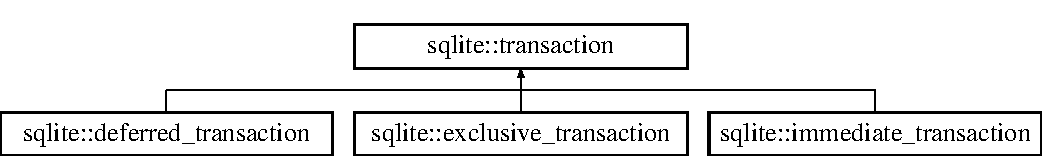
\includegraphics[height=2.000000cm]{a00014}
\end{center}
\end{figure}
\subsection*{Public Member Functions}
\begin{DoxyCompactItemize}
\item 
\hyperlink{a00014_ac5e2efbcd15f1531c00cbcacfa74c3f0}{transaction} (\hyperlink{a00004}{dbconnection} \&connection, const \hyperlink{a00038_aea994c2d3b1e9448cd9c526b44f78890}{Transaction\-Type} type)
\begin{DoxyCompactList}\small\item\em Implements a strictly scope-\/based S\-Q\-Lite transaction. \end{DoxyCompactList}\item 
virtual \hyperlink{a00014_a798101cf276674d19708c1958e5b03fb}{$\sim$transaction} () noexcept
\begin{DoxyCompactList}\small\item\em Destructor. \end{DoxyCompactList}\item 
\hypertarget{a00014_abe219dd0bf949d569381f9830c7b2d1a}{virtual void \hyperlink{a00014_abe219dd0bf949d569381f9830c7b2d1a}{commit} ()}\label{a00014_abe219dd0bf949d569381f9830c7b2d1a}

\begin{DoxyCompactList}\small\item\em Commit the transaction. \end{DoxyCompactList}\end{DoxyCompactItemize}


\subsection{Detailed Description}
R\-A\-I\-I encapsulation of the S\-Q\-Lite Transactions. 

Definition at line 26 of file Transaction.\-h.



\subsection{Constructor \& Destructor Documentation}
\hypertarget{a00014_ac5e2efbcd15f1531c00cbcacfa74c3f0}{\index{sqlite\-::transaction@{sqlite\-::transaction}!transaction@{transaction}}
\index{transaction@{transaction}!sqlite::transaction@{sqlite\-::transaction}}
\subsubsection[{transaction}]{\setlength{\rightskip}{0pt plus 5cm}sqlite\-::transaction\-::transaction (
\begin{DoxyParamCaption}
\item[{{\bf dbconnection} \&}]{connection, }
\item[{const {\bf Transaction\-Type}}]{type}
\end{DoxyParamCaption}
)}}\label{a00014_ac5e2efbcd15f1531c00cbcacfa74c3f0}


Implements a strictly scope-\/based S\-Q\-Lite transaction. 


\begin{DoxyParams}[1]{Parameters}
\mbox{\tt in}  & {\em connection} & the database connection to begin the transaction on \\
\hline
\mbox{\tt in}  & {\em type} & the transaction type to be used. \\
\hline
\end{DoxyParams}


Definition at line 10 of file Transaction.\-cpp.

\hypertarget{a00014_a798101cf276674d19708c1958e5b03fb}{\index{sqlite\-::transaction@{sqlite\-::transaction}!$\sim$transaction@{$\sim$transaction}}
\index{$\sim$transaction@{$\sim$transaction}!sqlite::transaction@{sqlite\-::transaction}}
\subsubsection[{$\sim$transaction}]{\setlength{\rightskip}{0pt plus 5cm}sqlite\-::transaction\-::$\sim$transaction (
\begin{DoxyParamCaption}
{}
\end{DoxyParamCaption}
)\hspace{0.3cm}{\ttfamily [virtual]}, {\ttfamily [noexcept]}}}\label{a00014_a798101cf276674d19708c1958e5b03fb}


Destructor. 

Safely rollback the transaction if it has not been commited. 

Definition at line 19 of file Transaction.\-cpp.



The documentation for this class was generated from the following files\-:\begin{DoxyCompactItemize}
\item 
src/\hyperlink{a00034}{Transaction.\-h}\item 
src/Transaction.\-cpp\end{DoxyCompactItemize}

\hypertarget{a00015}{\section{S\-Q\-Lite\-:\-:Value Class Reference}
\label{a00015}\index{S\-Q\-Lite\-::\-Value@{S\-Q\-Lite\-::\-Value}}
}


A \hyperlink{a00038}{S\-Q\-Lite} dynamically typed value object, aka \char`\"{}sqlite3\-\_\-value\char`\"{}.  




{\ttfamily \#include $<$Value.\-h$>$}

\subsection*{Public Member Functions}
\begin{DoxyCompactItemize}
\item 
\hyperlink{a00015_ace0be7092c23d5e3f4312db057d86997}{Value} (const sqlite3\-\_\-value $\ast$const value)
\begin{DoxyCompactList}\small\item\em Constructs a \hyperlink{a00015}{Value} object from a sqlite3\-\_\-value object. \end{DoxyCompactList}\item 
\hyperlink{a00015_acd6e10f2a509c8a0be20237d4b3a0fc7}{Value} (const \hyperlink{a00015}{Value} \&other)
\begin{DoxyCompactList}\small\item\em Copy constructor. \end{DoxyCompactList}\item 
\hyperlink{a00015_a531d4f514b9abe1eb1f47a277737b953}{Value} (\hyperlink{a00015}{Value} \&\&other)
\begin{DoxyCompactList}\small\item\em Move constructor. \end{DoxyCompactList}\item 
\hyperlink{a00015}{Value} \& \hyperlink{a00015_a879c07032f32606d277a8f6581a13abf}{operator=} (const \hyperlink{a00015}{Value} \&other)
\begin{DoxyCompactList}\small\item\em Copy assignment operator. \end{DoxyCompactList}\item 
\hyperlink{a00015}{Value} \& \hyperlink{a00015_ab80d7cf9eb8a462b23459d0fbba80277}{operator=} (\hyperlink{a00015}{Value} \&\&other)
\begin{DoxyCompactList}\small\item\em Move assignment operator. \end{DoxyCompactList}\item 
\hypertarget{a00015_adc0c8d347cbd6dbbd38c85ff755c9100}{sqlite3\-\_\-value $\ast$ \hyperlink{a00015_adc0c8d347cbd6dbbd38c85ff755c9100}{get\-Handle} () const noexcept}\label{a00015_adc0c8d347cbd6dbbd38c85ff755c9100}

\begin{DoxyCompactList}\small\item\em Returns pointer to the underlying \char`\"{}sqlite3\-\_\-value\char`\"{} object. \end{DoxyCompactList}\item 
int \hyperlink{a00015_a7dc198b9bcd56e1a00b4277d67e2fe94}{get\-Int} () const noexcept
\begin{DoxyCompactList}\small\item\em Represents the value as an integer. \end{DoxyCompactList}\item 
int64\-\_\-t \hyperlink{a00015_afea7de5c78253675c70f1d4c49740e37}{get\-Int64} () const noexcept
\begin{DoxyCompactList}\small\item\em Represents the value as a 64-\/bit integer. \end{DoxyCompactList}\item 
unsigned int \hyperlink{a00015_a196e4e06082b963730d766f99ccb3917}{get\-U\-Int} () const noexcept
\begin{DoxyCompactList}\small\item\em Represents the value as an unsigned integer. \end{DoxyCompactList}\item 
double \hyperlink{a00015_a7976bd8973e60229f32d57d80b309eef}{get\-Double} () const noexcept
\begin{DoxyCompactList}\small\item\em Represents the value as a double. \end{DoxyCompactList}\item 
const \hyperlink{a00002}{Blob} \hyperlink{a00015_a271c3d7f1de010f03197f5c72fd60d61}{get\-Blob} () const noexcept
\begin{DoxyCompactList}\small\item\em Represents the value as a blob object. \end{DoxyCompactList}\item 
const std\-::string \hyperlink{a00015_ae31b8ba26dec2668d11a49ad895e2267}{get\-String} () const noexcept
\begin{DoxyCompactList}\small\item\em Represents the value as a string. \end{DoxyCompactList}\item 
const std\-::u16string \hyperlink{a00015_a693c71ee6c918f92e4378e91318a7694}{get\-U16\-String} () const noexcept
\begin{DoxyCompactList}\small\item\em Represents the value as a U\-T\-F-\/16 string. \end{DoxyCompactList}\item 
int \hyperlink{a00015_a03a193504f0c5fd751302a6ec8d01845}{get\-Bytes} () const noexcept
\begin{DoxyCompactList}\small\item\em Returns the size in bytes of the value. \end{DoxyCompactList}\item 
\hyperlink{a00038_ad7a8ff5f375eca25eb6e3a51d746a04c}{Type} \hyperlink{a00015_ac43f7a22f87464aceaef9855e9700ff7}{get\-Type} () const noexcept
\begin{DoxyCompactList}\small\item\em Returns the Type for the inital datatype of the value. \end{DoxyCompactList}\end{DoxyCompactItemize}


\subsection{Detailed Description}
A \hyperlink{a00038}{S\-Q\-Lite} dynamically typed value object, aka \char`\"{}sqlite3\-\_\-value\char`\"{}. 

\hyperlink{a00015}{Value} objects represent all values that can be stored in a database table. A \hyperlink{a00015}{Value} object may be either \char`\"{}protected\char`\"{} or \char`\"{}unprotected\char`\"{} which refers to whether or not a mutex is held. An internal mutex is held for a protected value object but not for an unprotected one. If \hyperlink{a00038}{S\-Q\-Lite} is compiled to be single-\/threaded or if \hyperlink{a00038}{S\-Q\-Lite} is run in one of reduced mutex modes then there is no distinction between protected and unprotected sqlite3\-\_\-value objects. A \hyperlink{a00015}{Value} objects will always be \char`\"{}protected\char`\"{} as it stores a sqlite3\-\_\-value objects created from calling the sqlite3\-\_\-value\-\_\-dup() interface which produces a \char`\"{}protected\char`\"{} \char`\"{}sqlite3\-\_\-value\char`\"{} from an \char`\"{}unprotected\char`\"{} one. Only use a \hyperlink{a00015}{Value} object in the same thread as the S\-Q\-L function that created it. 

Definition at line 27 of file Value.\-h.



\subsection{Constructor \& Destructor Documentation}
\hypertarget{a00015_ace0be7092c23d5e3f4312db057d86997}{\index{S\-Q\-Lite\-::\-Value@{S\-Q\-Lite\-::\-Value}!Value@{Value}}
\index{Value@{Value}!SQLite::Value@{S\-Q\-Lite\-::\-Value}}
\subsubsection[{Value}]{\setlength{\rightskip}{0pt plus 5cm}S\-Q\-Lite\-::\-Value\-::\-Value (
\begin{DoxyParamCaption}
\item[{const sqlite3\-\_\-value $\ast$const}]{value}
\end{DoxyParamCaption}
)}}\label{a00015_ace0be7092c23d5e3f4312db057d86997}


Constructs a \hyperlink{a00015}{Value} object from a sqlite3\-\_\-value object. 


\begin{DoxyParams}[1]{Parameters}
\mbox{\tt in}  & {\em value} & a pointer to an sqlite3\-\_\-value object to initalize object with. \\
\hline
\end{DoxyParams}


Definition at line 6 of file Value.\-cpp.

\hypertarget{a00015_acd6e10f2a509c8a0be20237d4b3a0fc7}{\index{S\-Q\-Lite\-::\-Value@{S\-Q\-Lite\-::\-Value}!Value@{Value}}
\index{Value@{Value}!SQLite::Value@{S\-Q\-Lite\-::\-Value}}
\subsubsection[{Value}]{\setlength{\rightskip}{0pt plus 5cm}S\-Q\-Lite\-::\-Value\-::\-Value (
\begin{DoxyParamCaption}
\item[{const {\bf Value} \&}]{other}
\end{DoxyParamCaption}
)}}\label{a00015_acd6e10f2a509c8a0be20237d4b3a0fc7}


Copy constructor. 

Constructs a \hyperlink{a00015}{Value} object with a copy of the contents of other. 
\begin{DoxyParams}[1]{Parameters}
\mbox{\tt in}  & {\em other} & another \hyperlink{a00015}{Value} object to use as source to initialize object with. \\
\hline
\end{DoxyParams}


Definition at line 10 of file Value.\-cpp.

\hypertarget{a00015_a531d4f514b9abe1eb1f47a277737b953}{\index{S\-Q\-Lite\-::\-Value@{S\-Q\-Lite\-::\-Value}!Value@{Value}}
\index{Value@{Value}!SQLite::Value@{S\-Q\-Lite\-::\-Value}}
\subsubsection[{Value}]{\setlength{\rightskip}{0pt plus 5cm}S\-Q\-Lite\-::\-Value\-::\-Value (
\begin{DoxyParamCaption}
\item[{{\bf Value} \&\&}]{other}
\end{DoxyParamCaption}
)}}\label{a00015_a531d4f514b9abe1eb1f47a277737b953}


Move constructor. 

Constructs a \hyperlink{a00015}{Value} object with a copy of the contents of other using move semantics. 
\begin{DoxyParams}[1]{Parameters}
\mbox{\tt in}  & {\em other} & another \hyperlink{a00015}{Value} object to use as source to initialize object with. \\
\hline
\end{DoxyParams}


Definition at line 14 of file Value.\-cpp.



\subsection{Member Function Documentation}
\hypertarget{a00015_a271c3d7f1de010f03197f5c72fd60d61}{\index{S\-Q\-Lite\-::\-Value@{S\-Q\-Lite\-::\-Value}!get\-Blob@{get\-Blob}}
\index{get\-Blob@{get\-Blob}!SQLite::Value@{S\-Q\-Lite\-::\-Value}}
\subsubsection[{get\-Blob}]{\setlength{\rightskip}{0pt plus 5cm}const {\bf Blob} S\-Q\-Lite\-::\-Value\-::get\-Blob (
\begin{DoxyParamCaption}
{}
\end{DoxyParamCaption}
) const\hspace{0.3cm}{\ttfamily [noexcept]}}}\label{a00015_a271c3d7f1de010f03197f5c72fd60d61}


Represents the value as a blob object. 

\begin{DoxyReturn}{Returns}
A \hyperlink{a00002}{Blob} object representing the value of the object. 
\end{DoxyReturn}


Definition at line 56 of file Value.\-cpp.

\hypertarget{a00015_a03a193504f0c5fd751302a6ec8d01845}{\index{S\-Q\-Lite\-::\-Value@{S\-Q\-Lite\-::\-Value}!get\-Bytes@{get\-Bytes}}
\index{get\-Bytes@{get\-Bytes}!SQLite::Value@{S\-Q\-Lite\-::\-Value}}
\subsubsection[{get\-Bytes}]{\setlength{\rightskip}{0pt plus 5cm}int S\-Q\-Lite\-::\-Value\-::get\-Bytes (
\begin{DoxyParamCaption}
{}
\end{DoxyParamCaption}
) const\hspace{0.3cm}{\ttfamily [noexcept]}}}\label{a00015_a03a193504f0c5fd751302a6ec8d01845}


Returns the size in bytes of the value. 

\begin{DoxyReturn}{Returns}
The size in bytes of the value. 
\end{DoxyReturn}


Definition at line 74 of file Value.\-cpp.

\hypertarget{a00015_a7976bd8973e60229f32d57d80b309eef}{\index{S\-Q\-Lite\-::\-Value@{S\-Q\-Lite\-::\-Value}!get\-Double@{get\-Double}}
\index{get\-Double@{get\-Double}!SQLite::Value@{S\-Q\-Lite\-::\-Value}}
\subsubsection[{get\-Double}]{\setlength{\rightskip}{0pt plus 5cm}double S\-Q\-Lite\-::\-Value\-::get\-Double (
\begin{DoxyParamCaption}
{}
\end{DoxyParamCaption}
) const\hspace{0.3cm}{\ttfamily [noexcept]}}}\label{a00015_a7976bd8973e60229f32d57d80b309eef}


Represents the value as a double. 

\begin{DoxyReturn}{Returns}
A double representing the value of the object. 
\end{DoxyReturn}


Definition at line 51 of file Value.\-cpp.

\hypertarget{a00015_a7dc198b9bcd56e1a00b4277d67e2fe94}{\index{S\-Q\-Lite\-::\-Value@{S\-Q\-Lite\-::\-Value}!get\-Int@{get\-Int}}
\index{get\-Int@{get\-Int}!SQLite::Value@{S\-Q\-Lite\-::\-Value}}
\subsubsection[{get\-Int}]{\setlength{\rightskip}{0pt plus 5cm}int S\-Q\-Lite\-::\-Value\-::get\-Int (
\begin{DoxyParamCaption}
{}
\end{DoxyParamCaption}
) const\hspace{0.3cm}{\ttfamily [noexcept]}}}\label{a00015_a7dc198b9bcd56e1a00b4277d67e2fe94}


Represents the value as an integer. 

\begin{DoxyReturn}{Returns}
An integer representing the value of the object. 
\end{DoxyReturn}


Definition at line 36 of file Value.\-cpp.

\hypertarget{a00015_afea7de5c78253675c70f1d4c49740e37}{\index{S\-Q\-Lite\-::\-Value@{S\-Q\-Lite\-::\-Value}!get\-Int64@{get\-Int64}}
\index{get\-Int64@{get\-Int64}!SQLite::Value@{S\-Q\-Lite\-::\-Value}}
\subsubsection[{get\-Int64}]{\setlength{\rightskip}{0pt plus 5cm}int64\-\_\-t S\-Q\-Lite\-::\-Value\-::get\-Int64 (
\begin{DoxyParamCaption}
{}
\end{DoxyParamCaption}
) const\hspace{0.3cm}{\ttfamily [noexcept]}}}\label{a00015_afea7de5c78253675c70f1d4c49740e37}


Represents the value as a 64-\/bit integer. 

\begin{DoxyReturn}{Returns}
An 64-\/bit integer representing the value of the object. 
\end{DoxyReturn}


Definition at line 41 of file Value.\-cpp.

\hypertarget{a00015_ae31b8ba26dec2668d11a49ad895e2267}{\index{S\-Q\-Lite\-::\-Value@{S\-Q\-Lite\-::\-Value}!get\-String@{get\-String}}
\index{get\-String@{get\-String}!SQLite::Value@{S\-Q\-Lite\-::\-Value}}
\subsubsection[{get\-String}]{\setlength{\rightskip}{0pt plus 5cm}const std\-::string S\-Q\-Lite\-::\-Value\-::get\-String (
\begin{DoxyParamCaption}
{}
\end{DoxyParamCaption}
) const\hspace{0.3cm}{\ttfamily [noexcept]}}}\label{a00015_ae31b8ba26dec2668d11a49ad895e2267}


Represents the value as a string. 

\begin{DoxyReturn}{Returns}
A string representing the value of the object. 
\end{DoxyReturn}
\hypertarget{a00015_ac43f7a22f87464aceaef9855e9700ff7}{\index{S\-Q\-Lite\-::\-Value@{S\-Q\-Lite\-::\-Value}!get\-Type@{get\-Type}}
\index{get\-Type@{get\-Type}!SQLite::Value@{S\-Q\-Lite\-::\-Value}}
\subsubsection[{get\-Type}]{\setlength{\rightskip}{0pt plus 5cm}{\bf Type} S\-Q\-Lite\-::\-Value\-::get\-Type (
\begin{DoxyParamCaption}
{}
\end{DoxyParamCaption}
) const\hspace{0.3cm}{\ttfamily [noexcept]}}}\label{a00015_ac43f7a22f87464aceaef9855e9700ff7}


Returns the Type for the inital datatype of the value. 

Warning\-: Other interfaces might change the datatype for an \hyperlink{a00015}{Value} object. For example, if the datatype is initially \hyperlink{a00038_ad7a8ff5f375eca25eb6e3a51d746a04caa0faef0851b4294c06f2b94bb1cb2044}{S\-Q\-Lite\-::\-Type\-::\-Integer} and \hyperlink{a00015_ae31b8ba26dec2668d11a49ad895e2267}{get\-String()} is called to extract a text value for that integer, then subsequent calls to \hyperlink{a00015_ac43f7a22f87464aceaef9855e9700ff7}{get\-Type()} might return S\-Q\-Lite\-::\-Type\-::\-String. Whether or not a persistent internal datype conversion occurs is undefined and my change from one release of \hyperlink{a00038}{S\-Q\-Lite} to the nexxt. \begin{DoxyReturn}{Returns}
The type of the value. 
\end{DoxyReturn}


Definition at line 79 of file Value.\-cpp.

\hypertarget{a00015_a693c71ee6c918f92e4378e91318a7694}{\index{S\-Q\-Lite\-::\-Value@{S\-Q\-Lite\-::\-Value}!get\-U16\-String@{get\-U16\-String}}
\index{get\-U16\-String@{get\-U16\-String}!SQLite::Value@{S\-Q\-Lite\-::\-Value}}
\subsubsection[{get\-U16\-String}]{\setlength{\rightskip}{0pt plus 5cm}const std\-::u16string S\-Q\-Lite\-::\-Value\-::get\-U16\-String (
\begin{DoxyParamCaption}
{}
\end{DoxyParamCaption}
) const\hspace{0.3cm}{\ttfamily [noexcept]}}}\label{a00015_a693c71ee6c918f92e4378e91318a7694}


Represents the value as a U\-T\-F-\/16 string. 

\begin{DoxyReturn}{Returns}
A U\-T\-F-\/16 string representing the value of the object. 
\end{DoxyReturn}
\hypertarget{a00015_a196e4e06082b963730d766f99ccb3917}{\index{S\-Q\-Lite\-::\-Value@{S\-Q\-Lite\-::\-Value}!get\-U\-Int@{get\-U\-Int}}
\index{get\-U\-Int@{get\-U\-Int}!SQLite::Value@{S\-Q\-Lite\-::\-Value}}
\subsubsection[{get\-U\-Int}]{\setlength{\rightskip}{0pt plus 5cm}unsigned int S\-Q\-Lite\-::\-Value\-::get\-U\-Int (
\begin{DoxyParamCaption}
{}
\end{DoxyParamCaption}
) const\hspace{0.3cm}{\ttfamily [noexcept]}}}\label{a00015_a196e4e06082b963730d766f99ccb3917}


Represents the value as an unsigned integer. 

\begin{DoxyReturn}{Returns}
An unsigned integer representing the value of the object. 
\end{DoxyReturn}


Definition at line 46 of file Value.\-cpp.

\hypertarget{a00015_a879c07032f32606d277a8f6581a13abf}{\index{S\-Q\-Lite\-::\-Value@{S\-Q\-Lite\-::\-Value}!operator=@{operator=}}
\index{operator=@{operator=}!SQLite::Value@{S\-Q\-Lite\-::\-Value}}
\subsubsection[{operator=}]{\setlength{\rightskip}{0pt plus 5cm}{\bf Value} \& S\-Q\-Lite\-::\-Value\-::operator= (
\begin{DoxyParamCaption}
\item[{const {\bf Value} \&}]{other}
\end{DoxyParamCaption}
)}}\label{a00015_a879c07032f32606d277a8f6581a13abf}


Copy assignment operator. 

Replaces the contents with those of other. 
\begin{DoxyParams}[1]{Parameters}
\mbox{\tt in}  & {\em other} & another \hyperlink{a00015}{Value} object to use as source to initialize object with. \\
\hline
\end{DoxyParams}
\begin{DoxyReturn}{Returns}
$\ast$this 
\end{DoxyReturn}


Definition at line 22 of file Value.\-cpp.

\hypertarget{a00015_ab80d7cf9eb8a462b23459d0fbba80277}{\index{S\-Q\-Lite\-::\-Value@{S\-Q\-Lite\-::\-Value}!operator=@{operator=}}
\index{operator=@{operator=}!SQLite::Value@{S\-Q\-Lite\-::\-Value}}
\subsubsection[{operator=}]{\setlength{\rightskip}{0pt plus 5cm}{\bf Value} \& S\-Q\-Lite\-::\-Value\-::operator= (
\begin{DoxyParamCaption}
\item[{{\bf Value} \&\&}]{other}
\end{DoxyParamCaption}
)}}\label{a00015_ab80d7cf9eb8a462b23459d0fbba80277}


Move assignment operator. 

Replaces the contents with those of other using move semantics. 
\begin{DoxyParams}[1]{Parameters}
\mbox{\tt in}  & {\em other} & another \hyperlink{a00015}{Value} object to use as source to initialize object with. \\
\hline
\end{DoxyParams}
\begin{DoxyReturn}{Returns}
$\ast$this 
\end{DoxyReturn}


Definition at line 30 of file Value.\-cpp.



The documentation for this class was generated from the following files\-:\begin{DoxyCompactItemize}
\item 
src/\hyperlink{a00037}{Value.\-h}\item 
src/Value.\-cpp\end{DoxyCompactItemize}

\chapter{File Documentation}
\hypertarget{a00018}{\section{src/\-Backup.h File Reference}
\label{a00018}\index{src/\-Backup.\-h@{src/\-Backup.\-h}}
}
{\ttfamily \#include \char`\"{}D\-B\-Connection.\-h\char`\"{}}\\*
{\ttfamily \#include $<$sqlite3.\-h$>$}\\*
{\ttfamily \#include $<$memory$>$}\\*
\subsection*{Classes}
\begin{DoxyCompactItemize}
\item 
class \hyperlink{a00001}{sqlite\-::backup}
\begin{DoxyCompactList}\small\item\em Used to aid in the process of backing up a database. \end{DoxyCompactList}\end{DoxyCompactItemize}
\subsection*{Namespaces}
\begin{DoxyCompactItemize}
\item 
\hyperlink{a00038}{sqlite}
\begin{DoxyCompactList}\small\item\em S\-Q\-Lite\-X\-X classes and functions are defined in this namespace. \end{DoxyCompactList}\end{DoxyCompactItemize}

\hypertarget{a00020}{\section{src/\-Blob.h File Reference}
\label{a00020}\index{src/\-Blob.\-h@{src/\-Blob.\-h}}
}
{\ttfamily \#include $<$sqlite3.\-h$>$}\\*
{\ttfamily \#include $<$cassert$>$}\\*
{\ttfamily \#include $<$cstring$>$}\\*
{\ttfamily \#include $<$memory$>$}\\*
{\ttfamily \#include $<$utility$>$}\\*
\subsection*{Classes}
\begin{DoxyCompactItemize}
\item 
class \hyperlink{a00002}{S\-Q\-Lite\-::\-Blob}
\begin{DoxyCompactList}\small\item\em A \char`\"{}\-Binary Large O\-Bject\char`\"{}. \end{DoxyCompactList}\end{DoxyCompactItemize}
\subsection*{Namespaces}
\begin{DoxyCompactItemize}
\item 
\hyperlink{a00038}{S\-Q\-Lite}
\begin{DoxyCompactList}\small\item\em S\-Q\-Lite\-X\-X classes and functions are defined in this namespace. \end{DoxyCompactList}\end{DoxyCompactItemize}

\hypertarget{a00022}{\section{src/\-D\-B\-Connection.h File Reference}
\label{a00022}\index{src/\-D\-B\-Connection.\-h@{src/\-D\-B\-Connection.\-h}}
}
{\ttfamily \#include \char`\"{}Exception.\-h\char`\"{}}\\*
{\ttfamily \#include \char`\"{}Functions.\-h\char`\"{}}\\*
{\ttfamily \#include \char`\"{}Mutex.\-h\char`\"{}}\\*
{\ttfamily \#include \char`\"{}Open.\-h\char`\"{}}\\*
{\ttfamily \#include $<$sqlite3.\-h$>$}\\*
{\ttfamily \#include $<$cassert$>$}\\*
{\ttfamily \#include $<$chrono$>$}\\*
{\ttfamily \#include $<$memory$>$}\\*
{\ttfamily \#include $<$thread$>$}\\*
\subsection*{Classes}
\begin{DoxyCompactItemize}
\item 
class \hyperlink{a00004}{sqlite\-::dbconnection}
\begin{DoxyCompactList}\small\item\em Class that represents a connection to a database. \end{DoxyCompactList}\end{DoxyCompactItemize}
\subsection*{Namespaces}
\begin{DoxyCompactItemize}
\item 
\hyperlink{a00038}{sqlite}
\begin{DoxyCompactList}\small\item\em S\-Q\-Lite\-X\-X classes and functions are defined in this namespace. \end{DoxyCompactList}\end{DoxyCompactItemize}

\hypertarget{a00024}{\section{src/\-Exception.h File Reference}
\label{a00024}\index{src/\-Exception.\-h@{src/\-Exception.\-h}}
}
{\ttfamily \#include $<$sqlite3.\-h$>$}\\*
{\ttfamily \#include $<$stdexcept$>$}\\*
{\ttfamily \#include $<$string$>$}\\*
\subsection*{Classes}
\begin{DoxyCompactItemize}
\item 
class \hyperlink{a00006}{S\-Q\-Lite\-::\-Exception}
\begin{DoxyCompactList}\small\item\em Encapsulation of the error code and message from S\-Q\-Lite3, based on std\-::runtime\-\_\-error. \end{DoxyCompactList}\item 
class \hyperlink{a00003}{S\-Q\-Lite\-::\-Busy\-Exception}
\begin{DoxyCompactList}\small\item\em Encapsulation of the S\-Q\-L\-I\-T\-E\-\_\-\-B\-U\-S\-Y error code derived from \hyperlink{a00006}{S\-Q\-Lite\-::\-Exception}. \end{DoxyCompactList}\end{DoxyCompactItemize}
\subsection*{Namespaces}
\begin{DoxyCompactItemize}
\item 
\hyperlink{a00038}{S\-Q\-Lite}
\begin{DoxyCompactList}\small\item\em S\-Q\-Lite\-X\-X classes and functions are defined in this namespace. \end{DoxyCompactList}\end{DoxyCompactItemize}

\hypertarget{a00027}{\section{src/\-Mutex.h File Reference}
\label{a00027}\index{src/\-Mutex.\-h@{src/\-Mutex.\-h}}
}
{\ttfamily \#include $<$sqlite3.\-h$>$}\\*
\subsection*{Classes}
\begin{DoxyCompactItemize}
\item 
class \hyperlink{a00009}{sqlite\-::mutex}
\begin{DoxyCompactList}\small\item\em Helps with serializing access to a database connection. \end{DoxyCompactList}\end{DoxyCompactItemize}

\hypertarget{a00028}{\section{src/\-Open.h File Reference}
\label{a00028}\index{src/\-Open.\-h@{src/\-Open.\-h}}
}
{\ttfamily \#include $<$sqlite3.\-h$>$}\\*
{\ttfamily \#include $<$type\-\_\-traits$>$}\\*
\subsection*{Namespaces}
\begin{DoxyCompactItemize}
\item 
\hyperlink{a00038}{sqlite}
\begin{DoxyCompactList}\small\item\em S\-Q\-Lite\-X\-X classes and functions are defined in this namespace. \end{DoxyCompactList}\end{DoxyCompactItemize}
\subsection*{Enumerations}
\begin{DoxyCompactItemize}
\item 
enum \hyperlink{a00038_ac886eded97b0430b2ab92e2d08fcf938}{sqlite\-::openmode} \-: int \{ \\*
\hyperlink{a00038_ac886eded97b0430b2ab92e2d08fcf938abefe72871b2de8f4f0e20108517e31fe}{sqlite\-::openmode\-::read\-\_\-only} = S\-Q\-L\-I\-T\-E\-\_\-\-O\-P\-E\-N\-\_\-\-R\-E\-A\-D\-O\-N\-L\-Y, 
\hyperlink{a00038_ac886eded97b0430b2ab92e2d08fcf938a06ad287ea83b37a6f9db3d8d10d72c8f}{sqlite\-::openmode\-::read\-\_\-write} = S\-Q\-L\-I\-T\-E\-\_\-\-O\-P\-E\-N\-\_\-\-R\-E\-A\-D\-W\-R\-I\-T\-E, 
\hyperlink{a00038_ac886eded97b0430b2ab92e2d08fcf938a76ea0bebb3c22822b4f0dd9c9fd021c5}{sqlite\-::openmode\-::create} = S\-Q\-L\-I\-T\-E\-\_\-\-O\-P\-E\-N\-\_\-\-C\-R\-E\-A\-T\-E, 
\hyperlink{a00038_ac886eded97b0430b2ab92e2d08fcf938a9305b73d359bd06734fee0b3638079e1}{sqlite\-::openmode\-::uri} = S\-Q\-L\-I\-T\-E\-\_\-\-O\-P\-E\-N\-\_\-\-U\-R\-I, 
\\*
\hyperlink{a00038_ac886eded97b0430b2ab92e2d08fcf938acd69b4957f06cd818d7bf3d61980e291}{sqlite\-::openmode\-::memory} = S\-Q\-L\-I\-T\-E\-\_\-\-O\-P\-E\-N\-\_\-\-M\-E\-M\-O\-R\-Y, 
\hyperlink{a00038_ac886eded97b0430b2ab92e2d08fcf938afb79f3efe5bfb497a2fdd85aca8a73bb}{sqlite\-::openmode\-::no\-\_\-mutex} = S\-Q\-L\-I\-T\-E\-\_\-\-O\-P\-E\-N\-\_\-\-N\-O\-M\-U\-T\-E\-X, 
\hyperlink{a00038_ac886eded97b0430b2ab92e2d08fcf938addc995071d9f139c13354c2839603fac}{sqlite\-::openmode\-::full\-\_\-mutex} = S\-Q\-L\-I\-T\-E\-\_\-\-O\-P\-E\-N\-\_\-\-F\-U\-L\-L\-M\-U\-T\-E\-X, 
\hyperlink{a00038_ac886eded97b0430b2ab92e2d08fcf938a799bb323b5a99b0e122ba5aec784d314}{sqlite\-::openmode\-::shared\-\_\-cache} = S\-Q\-L\-I\-T\-E\-\_\-\-O\-P\-E\-N\-\_\-\-S\-H\-A\-R\-E\-D\-C\-A\-C\-H\-E, 
\\*
\hyperlink{a00038_ac886eded97b0430b2ab92e2d08fcf938a56ffbad7684376d679b1f0dcf37d8bf7}{sqlite\-::openmode\-::private\-\_\-cache} = S\-Q\-L\-I\-T\-E\-\_\-\-O\-P\-E\-N\-\_\-\-P\-R\-I\-V\-A\-T\-E\-C\-A\-C\-H\-E
 \}
\begin{DoxyCompactList}\small\item\em Different ways to open a dbconnection. \end{DoxyCompactList}\end{DoxyCompactItemize}

\hypertarget{a00029}{\section{src/\-S\-Q\-Lite\-Enums.h File Reference}
\label{a00029}\index{src/\-S\-Q\-Lite\-Enums.\-h@{src/\-S\-Q\-Lite\-Enums.\-h}}
}
{\ttfamily \#include $<$sqlite3.\-h$>$}\\*
\subsection*{Namespaces}
\begin{DoxyCompactItemize}
\item 
\hyperlink{a00038}{S\-Q\-Lite}
\begin{DoxyCompactList}\small\item\em S\-Q\-Lite\-X\-X classes and functions are defined in this namespace. \end{DoxyCompactList}\end{DoxyCompactItemize}
\subsection*{Enumerations}
\begin{DoxyCompactItemize}
\item 
enum \hyperlink{a00038_ad7a8ff5f375eca25eb6e3a51d746a04c}{S\-Q\-Lite\-::\-Type} \-: int \{ \\*
\hyperlink{a00038_ad7a8ff5f375eca25eb6e3a51d746a04caa0faef0851b4294c06f2b94bb1cb2044}{S\-Q\-Lite\-::\-Type\-::\-Integer} = S\-Q\-L\-I\-T\-E\-\_\-\-I\-N\-T\-E\-G\-E\-R, 
\hyperlink{a00038_ad7a8ff5f375eca25eb6e3a51d746a04ca22ae0e2b89e5e3d477f988cc36d3272b}{S\-Q\-Lite\-::\-Type\-::\-Float} = S\-Q\-L\-I\-T\-E\-\_\-\-F\-L\-O\-A\-T, 
\hyperlink{a00038_ad7a8ff5f375eca25eb6e3a51d746a04cae8016c85ada38bdc5fac616ec1318047}{S\-Q\-Lite\-::\-Type\-::\-Blob} = S\-Q\-L\-I\-T\-E\-\_\-\-B\-L\-O\-B, 
\hyperlink{a00038_ad7a8ff5f375eca25eb6e3a51d746a04cabbb93ef26e3c101ff11cdd21cab08a94}{S\-Q\-Lite\-::\-Type\-::\-Null} = S\-Q\-L\-I\-T\-E\-\_\-\-N\-U\-L\-L, 
\\*
\hyperlink{a00038_ad7a8ff5f375eca25eb6e3a51d746a04ca9dffbf69ffba8bc38bc4e01abf4b1675}{S\-Q\-Lite\-::\-Type\-::\-Text} = S\-Q\-L\-I\-T\-E3\-\_\-\-T\-E\-X\-T
 \}
\begin{DoxyCompactList}\small\item\em Every value in \hyperlink{a00038}{S\-Q\-Lite} has one of the following fundamental datatypes. \end{DoxyCompactList}\item 
enum \hyperlink{a00038_a32877e51b309dd8f2a28c21c0ba4a6fd}{S\-Q\-Lite\-::\-Bind\-Type} \-: int \{ \hyperlink{a00038_a32877e51b309dd8f2a28c21c0ba4a6fda84a8921b25f505d0d2077aeb5db4bc16}{S\-Q\-Lite\-::\-Bind\-Type\-::\-Static}, 
\hyperlink{a00038_a32877e51b309dd8f2a28c21c0ba4a6fdab1f023eff9a6b5308d6024e4c6b3d475}{S\-Q\-Lite\-::\-Bind\-Type\-::\-Transient}
 \}
\begin{DoxyCompactList}\small\item\em Used to specify the way to bind a value to a statement. \end{DoxyCompactList}\end{DoxyCompactItemize}

\hypertarget{a00030}{\section{src/\-S\-Q\-Lite\-X\-X.h File Reference}
\label{a00030}\index{src/\-S\-Q\-Lite\-X\-X.\-h@{src/\-S\-Q\-Lite\-X\-X.\-h}}
}
{\ttfamily \#include \char`\"{}Backup.\-h\char`\"{}}\\*
{\ttfamily \#include \char`\"{}D\-B\-Connection.\-h\char`\"{}}\\*
{\ttfamily \#include \char`\"{}Exception.\-h\char`\"{}}\\*
{\ttfamily \#include \char`\"{}Functions.\-h\char`\"{}}\\*
{\ttfamily \#include \char`\"{}Open.\-h\char`\"{}}\\*
{\ttfamily \#include \char`\"{}Statement.\-h\char`\"{}}\\*
{\ttfamily \#include \char`\"{}Transaction.\-h\char`\"{}}\\*
{\ttfamily \#include $<$sqlite3.\-h$>$}\\*
\subsection*{Namespaces}
\begin{DoxyCompactItemize}
\item 
\hyperlink{a00038}{sqlite}
\begin{DoxyCompactList}\small\item\em S\-Q\-Lite\-X\-X classes and functions are defined in this namespace. \end{DoxyCompactList}\end{DoxyCompactItemize}

\hypertarget{a00032}{\section{src/\-Statement.h File Reference}
\label{a00032}\index{src/\-Statement.\-h@{src/\-Statement.\-h}}
}
{\ttfamily \#include \char`\"{}Blob.\-h\char`\"{}}\\*
{\ttfamily \#include \char`\"{}D\-B\-Connection.\-h\char`\"{}}\\*
{\ttfamily \#include \char`\"{}S\-Q\-Lite\-Enums.\-h\char`\"{}}\\*
{\ttfamily \#include \char`\"{}Value.\-h\char`\"{}}\\*
{\ttfamily \#include $<$sqlite3.\-h$>$}\\*
{\ttfamily \#include $<$cassert$>$}\\*
{\ttfamily \#include $<$cstring$>$}\\*
{\ttfamily \#include $<$functional$>$}\\*
{\ttfamily \#include $<$iostream$>$}\\*
{\ttfamily \#include $<$map$>$}\\*
{\ttfamily \#include $<$memory$>$}\\*
{\ttfamily \#include $<$string$>$}\\*
{\ttfamily \#include $<$utility$>$}\\*
{\ttfamily \#include $<$vector$>$}\\*
{\ttfamily \#include $<$limits.\-h$>$}\\*
\subsection*{Classes}
\begin{DoxyCompactItemize}
\item 
class \hyperlink{a00010}{sqlite\-::reader$<$ T $>$}
\begin{DoxyCompactList}\small\item\em Base class used to help with reading \char`\"{}sqlite3\-\_\-stmt\char`\"{} information. \end{DoxyCompactList}\item 
class \hyperlink{a00011}{sqlite\-::row}
\begin{DoxyCompactList}\small\item\em Represents a returned row when stepping through a \char`\"{}\-S\-E\-L\-E\-C\-T\char`\"{} statement. \end{DoxyCompactList}\item 
class \hyperlink{a00013}{sqlite\-::statement}
\begin{DoxyCompactList}\small\item\em Represents a single S\-Q\-L statement that has been compiled into binary form and is ready to be evaluated, aka \char`\"{}sqlite3\-\_\-stmt\char`\"{}. \end{DoxyCompactList}\item 
class \hyperlink{a00012}{sqlite\-::row\-\_\-iterator}
\begin{DoxyCompactList}\small\item\em Helps when iterating over rows in a \char`\"{}\-S\-E\-L\-E\-C\-T\char`\"{} statement. \end{DoxyCompactList}\end{DoxyCompactItemize}
\subsection*{Namespaces}
\begin{DoxyCompactItemize}
\item 
\hyperlink{a00038}{sqlite}
\begin{DoxyCompactList}\small\item\em S\-Q\-Lite\-X\-X classes and functions are defined in this namespace. \end{DoxyCompactList}\end{DoxyCompactItemize}
\subsection*{Functions}
\begin{DoxyCompactItemize}
\item 
row\-\_\-iterator \hyperlink{a00038_a82c17565b2423a151a79f500e05384c7}{sqlite\-::begin} (const statement \&statement) noexcept
\begin{DoxyCompactList}\small\item\em Returns an iterator to the first row of a statement. \end{DoxyCompactList}\item 
row\-\_\-iterator \hyperlink{a00038_a9bb86a852a764bb601061807c9c53107}{sqlite\-::end} (const statement \&statement) noexcept
\begin{DoxyCompactList}\small\item\em Returns an iterator to the end. \end{DoxyCompactList}\item 
{\footnotesize template$<$typename... Values$>$ }\\int \hyperlink{a00038_ac3634536982adcefd80f2e5b5a8a105d}{sqlite\-::execute} (const dbconnection \&connection, const std\-::string \&text, Values \&\&...values)
\begin{DoxyCompactList}\small\item\em Executes an S\-Q\-L query on a database connection. \end{DoxyCompactList}\item 
{\footnotesize template$<$typename... Values$>$ }\\int \hyperlink{a00038_a5d8cb158ff2ea9cd6331c9ed8dfde8da}{sqlite\-::execute} (const dbconnection \&connection, const std\-::u16string \&text, Values \&\&...values)
\begin{DoxyCompactList}\small\item\em Executes an S\-Q\-L query on a database connection. \end{DoxyCompactList}\end{DoxyCompactItemize}

\hypertarget{a00034}{\section{src/\-Transaction.h File Reference}
\label{a00034}\index{src/\-Transaction.\-h@{src/\-Transaction.\-h}}
}
{\ttfamily \#include \char`\"{}D\-B\-Connection.\-h\char`\"{}}\\*
{\ttfamily \#include \char`\"{}Statement.\-h\char`\"{}}\\*
{\ttfamily \#include $<$sqlite3.\-h$>$}\\*
\subsection*{Classes}
\begin{DoxyCompactItemize}
\item 
class \hyperlink{a00014}{S\-Q\-Lite\-::\-Transaction}
\begin{DoxyCompactList}\small\item\em R\-A\-I\-I encapsulation of the \hyperlink{a00038}{S\-Q\-Lite} Transactions. \end{DoxyCompactList}\item 
class \hyperlink{a00005}{S\-Q\-Lite\-::\-Deferred\-Transaction}
\begin{DoxyCompactList}\small\item\em R\-A\-I\-I encapsulation of the \hyperlink{a00038}{S\-Q\-Lite} deferred transaction. \end{DoxyCompactList}\item 
class \hyperlink{a00008}{S\-Q\-Lite\-::\-Immediate\-Transaction}
\begin{DoxyCompactList}\small\item\em R\-A\-I\-I encapsulation of the \hyperlink{a00038}{S\-Q\-Lite} immediate transaction. \end{DoxyCompactList}\item 
class \hyperlink{a00007}{S\-Q\-Lite\-::\-Exclusive\-Transaction}
\begin{DoxyCompactList}\small\item\em R\-A\-I\-I encapsulation of the \hyperlink{a00038}{S\-Q\-Lite} exclusive transaction. \end{DoxyCompactList}\end{DoxyCompactItemize}
\subsection*{Namespaces}
\begin{DoxyCompactItemize}
\item 
\hyperlink{a00038}{S\-Q\-Lite}
\begin{DoxyCompactList}\small\item\em S\-Q\-Lite\-X\-X classes and functions are defined in this namespace. \end{DoxyCompactList}\end{DoxyCompactItemize}
\subsection*{Enumerations}
\begin{DoxyCompactItemize}
\item 
enum \hyperlink{a00038_af94f2dd6dcae8699eada7a0382e48e66}{S\-Q\-Lite\-::\-Transaction\-Type} \-: int \{ \hyperlink{a00038_af94f2dd6dcae8699eada7a0382e48e66a4ed71db54748b36eeb398876b0c747ac}{S\-Q\-Lite\-::\-Transaction\-Type\-::\-Deferred}, 
\hyperlink{a00038_af94f2dd6dcae8699eada7a0382e48e66a43f6615bbb2c40a5306ff804094420b1}{S\-Q\-Lite\-::\-Transaction\-Type\-::\-Immediate}, 
\hyperlink{a00038_af94f2dd6dcae8699eada7a0382e48e66a2ef50b4c466304dc6ac77bac8a779971}{S\-Q\-Lite\-::\-Transaction\-Type\-::\-Exclusive}
 \}
\begin{DoxyCompactList}\small\item\em Used to specify the different types of \hyperlink{a00038}{S\-Q\-Lite} transactions. \end{DoxyCompactList}\end{DoxyCompactItemize}

\hypertarget{a00037}{\section{src/\-Value.h File Reference}
\label{a00037}\index{src/\-Value.\-h@{src/\-Value.\-h}}
}
{\ttfamily \#include \char`\"{}S\-Q\-Lite\-Enums.\-h\char`\"{}}\\*
{\ttfamily \#include \char`\"{}Blob.\-h\char`\"{}}\\*
{\ttfamily \#include $<$sqlite3.\-h$>$}\\*
{\ttfamily \#include $<$cassert$>$}\\*
{\ttfamily \#include $<$cstring$>$}\\*
{\ttfamily \#include $<$string$>$}\\*
\subsection*{Classes}
\begin{DoxyCompactItemize}
\item 
class \hyperlink{a00015}{S\-Q\-Lite\-::\-Value}
\begin{DoxyCompactList}\small\item\em A \hyperlink{a00038}{S\-Q\-Lite} dynamically typed value object, aka \char`\"{}sqlite3\-\_\-value\char`\"{}. \end{DoxyCompactList}\end{DoxyCompactItemize}
\subsection*{Namespaces}
\begin{DoxyCompactItemize}
\item 
\hyperlink{a00038}{S\-Q\-Lite}
\begin{DoxyCompactList}\small\item\em S\-Q\-Lite\-X\-X classes and functions are defined in this namespace. \end{DoxyCompactList}\end{DoxyCompactItemize}

%--- End generated contents ---

% Index
\newpage
\phantomsection
\addcontentsline{toc}{chapter}{Index}
\printindex

\end{document}
